\chapter{Case Study thực tế (phần 1)}

\section{\textbf{Dự án 1: Tạo short video hoạt hình bằng AI và đăng lên youtube }}

\href{https://drive.google.com/file/d/1hBEgM7DZBiMOocM_pxGyne7T97oAKK_B/view?usp=sharing}{\textbf{\underline {Link tải workflow}}}

\begin{figure}[h]
    \centering
    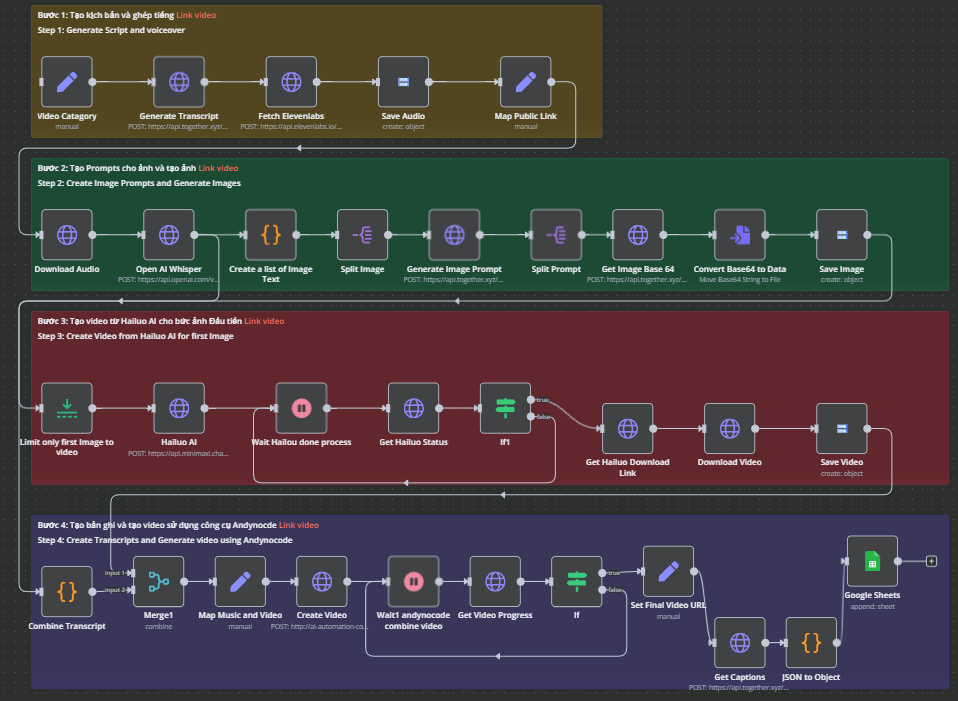
\includegraphics[width=1\textwidth]{images/Da1-01.png}
    \caption{Workflow kết quả dự án 1}
    
\end{figure}

Trong ví dụ này chúng ta sẽ làm một workflow để tạo short video animated. \\

\underline{Ứng dụng:}\\
\begin{itemize}[label=-]
    \item Nhà tiếp thị muốn tạo video quảng cáo tự động, nhanh chóng
    \item Người sáng tạo nội dung muốn tối ưu hóa quy trình sản xuất video
    \item Doanh nghiệp tìm kiếm phương pháp hiệu quả để giới thiệu sản phẩm 
\end{itemize}


\underline{Ý tưởng thiết kế:}\\
\begin{figure}[h]
    \centering
    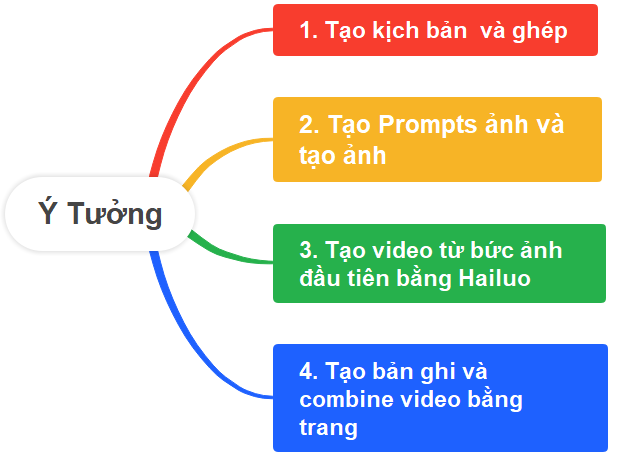
\includegraphics[width=0.7\textwidth]{images/Da1-02.png}
    \caption{Ý tưởng thiết kế}
    
\end{figure}


\underline{Các công cụ sử dụng trong workflow:}\\
\begin{itemize}[label=-]
    \item \textbf{Tạo giọng nói AI với ElevenLabs}: Sử dụng \textbf{\emph{ElevenLabs}}, quy trình này chuyển đổi văn bản thành giọng nói tự nhiên, giúp video trở nên sống động và chuyên nghiệp hơn. ElevenLabs AI là một nền tảng AI Text-to-Speech (TTS) giúp chuyển đổi văn bản thành giọng nói tự nhiên, chân thực với nhiều giọng đọc và ngôn ngữ khác nhau. Nó thường được dùng để tạo giọng nói nhân tạo phục vụ video, podcast, ứng dụng AI, chatbot và nhiều mục đích khác. ElevenLabs AI giúp tự động hóa quy trình tạo giọng nói từ văn bản. Dùng trong một số ứng dụng thực tế như: Chuyển đổi văn bản thành giọng nói (TTS) tự động, Tạo chatbot có giọng nói nhân tạo, Đọc báo, thông tin hoặc tin tức tự động, Tổng đài AI tự động (Voice AI Callbot)
    \item \textbf{Chuyển đổi ảnh thành video với Hailuo AI}: Với  \textbf{\emph{Hailuo AI}} hình ảnh tĩnh được chuyển đổi thành video động, giúp tạo nội dung trực quan hấp dẫn mà không cần chỉnh sửa thủ công. Các ứng dụng mà Hailou AI có thể làm.\\

    + Chuyển đổi văn bản thành video: Hailuo AI giúp biến những đoạn văn bản thành video sống động, tối ưu hóa quy trình sáng tạo nội dung và tiết kiệm thời gian cho người dùng.\\
    + Chuyển đổi hình ảnh thành video: Người dùng có thể tải lên hình ảnh tĩnh và nhập mô tả; Hailuo AI sẽ tạo ra video dựa trên nội dung đó, mang lại trải nghiệm trực quan và sinh động.\\
    + Chuyển đổi văn bản thành giọng nói (Text-to-Speech): Hailuo AI cung cấp tính năng chuyển đổi văn bản thành giọng nói với nhiều ngôn ngữ và giọng đọc tự nhiên, hỗ trợ đa dạng nhu cầu của người dùng. 
    \item \textbf{Cải thiện nội dung với Together AI}: Để đảm bảo chất lượng nội dung cao, \textbf{\emph{Together AI}} tối ưu hóa và điều chỉnh lời nhắc, giúp tạo ra các kịch bản hấp dẫn và phù hợp hơn. Nó giống một bên trung gian để chung ta truy cập vào các mô hình AI.
    \item \textbf{Xử lý thông minh với OpenAI}: Các tác vụ suy luận, như tạo nội dung văn bản và tối ưu hóa nội dung, được thực hiện bởi \textbf{\emph{OpenAI}}, giúp quy trình sản xuất video diễn ra trơn tru và hiệu quả. 
    \item \textbf{Tích hợp với Google Sheets}: Sau khi tạo video, \textbf{\emph{URL tải xuống}} sẽ được tự động tải lên \textbf{\emph{Google Sheets}}, giúp người dùng dễ dàng truy cập và quản lý nội dung. 
     \item \textbf{Lưu trữ thông tin bằng Google Cloud Storage}: Node \textbf{\emph{Google Cloud Storage}} trong n8n giúp bạn làm việc với dịch vụ lưu trữ đám mây Google Cloud Storage (GCS). Nó cho phép bạn tải lên, tải xuống, xóa và quản lý tệp trên Google Cloud Storage Buckets trong quy trình tự động hóa của mình. 
     \item \textbf{Tối ưu hóa với node code}: Node Code trong n8n cho phép bạn viết JavaScript để xử lý dữ liệu tùy chỉnh trong quy trình tự động hóa. Nó giúp mở rộng khả năng của n8n khi các node có sẵn không đáp ứng đủ nhu cầu.   
\end{itemize}

\underline{\textbf{ Các bước triển khai:}}

\subsection{Tạo node "Edit Fields}

\begin{itemize}
    \item[-] Tạo các trường dữ liệu (data fields): Node Edit File cho phép tạo ra các trường dữ liệu mới và gán giá trị cho chúng.
    \item[-] Mapping (ánh xạ) dữ liệu: Node Edit File được sử dụng để ánh xạ dữ liệu từ các nguồn khác nhau và kết hợp chúng lại với nhau. Ví dụ: Ánh xạ URL của audio đã tạo, Kết hợp URL của video và nhạc nền. Thiết lập các tham số (parameters): Node Edit File được sử dụng để thiết lập các tham số cần thiết cho các bước tiếp theo trong quy trình.
    \item[-] Chỉnh sửa thông tin: Node Edit File có thể chỉnh sửa các thông tin khác nhau.
\end{itemize}  
    \begin{figure}[H]
 
    \centering
    \begin{minipage}{0.5\textwidth}
        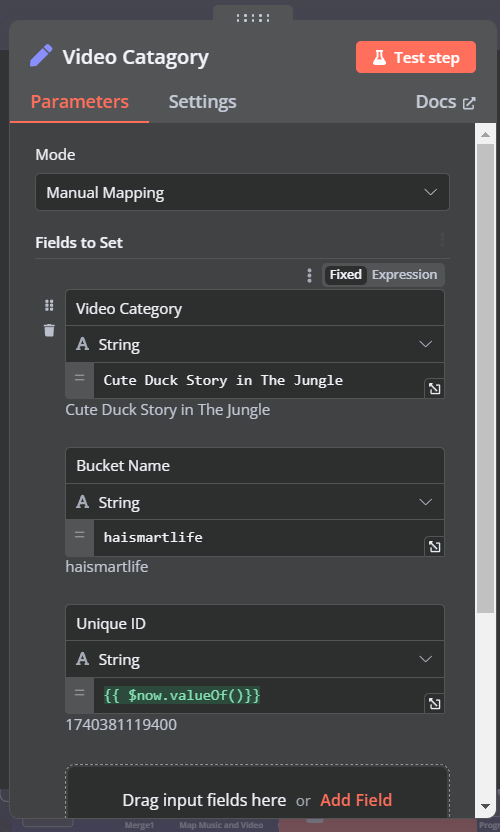
\includegraphics[width=\linewidth]{images/Da1-03.png}
    \end{minipage}
    %\hfill
    \hspace{5pt}
    \begin{minipage}{0.4\textwidth}
    
        \underline{Các thông số cần cài đặt:}\\
        \begin{itemize}[label=\textbullet]
            \item Đổi tên node thành \emph{"Video Catagory"}
            \item Mục Mode: Chọn \emph{"Manual Mapping"}
            \item Mục Fields to Set: Chọn "Add Field" và tạo 3 trường như hình bên cạnh, trong đó:\\
            
            \textbf{\emph{"Video Category"}} là trường  nội dung video bạn muốn tạo, thay thế thành loại video hoặc nội dung bạn muốn.\\
            \textbf{\emph{"Bucket Name"}} là tên của bucket mà bạn sẽ tạo trong google cloud để lưu các hình ảnh, âm thanh AI tạo ra.\\
            \textbf{\emph{"Unique ID"}} bằng giá trị "\verb|{{$now.valueOf()}}|" là một tham số quan trọng để đảm bảo tính duy nhất và chính xác của các tệp trong quy trình tạo video tự động, đặc biệt là để ngăn chặn các vấn đề liên quan đến caching.\\

            
        \end{itemize}
    \end{minipage}
\end{figure}
     
    % \item 
    % \item 
    % \item 
    % \item 


\subsection{Elevenlabs - AI về âm thanh, chuyển đổi text và voice.}
\begin{itemize}[label=]
    \item \textbf{Bước 1: Tạo API key Elevenlabs} 
    
    Truy cập vào link \url{https://elevenlabs.io/app/settings/api-keys} \\ 
    
    Tìm đến API key và nhấn tạo ta sẽ được dãy ký tự, sau đó hãy copy nó.\\
    
    Lưu ý: API này dùng free sẽ hay bị lỗi nên nếu xây dựng được một workflow hữu ích thì nên mua để tránh gặp các lỗi không mong muốn.\\
    
    \begin{figure}[H]
    \centering
    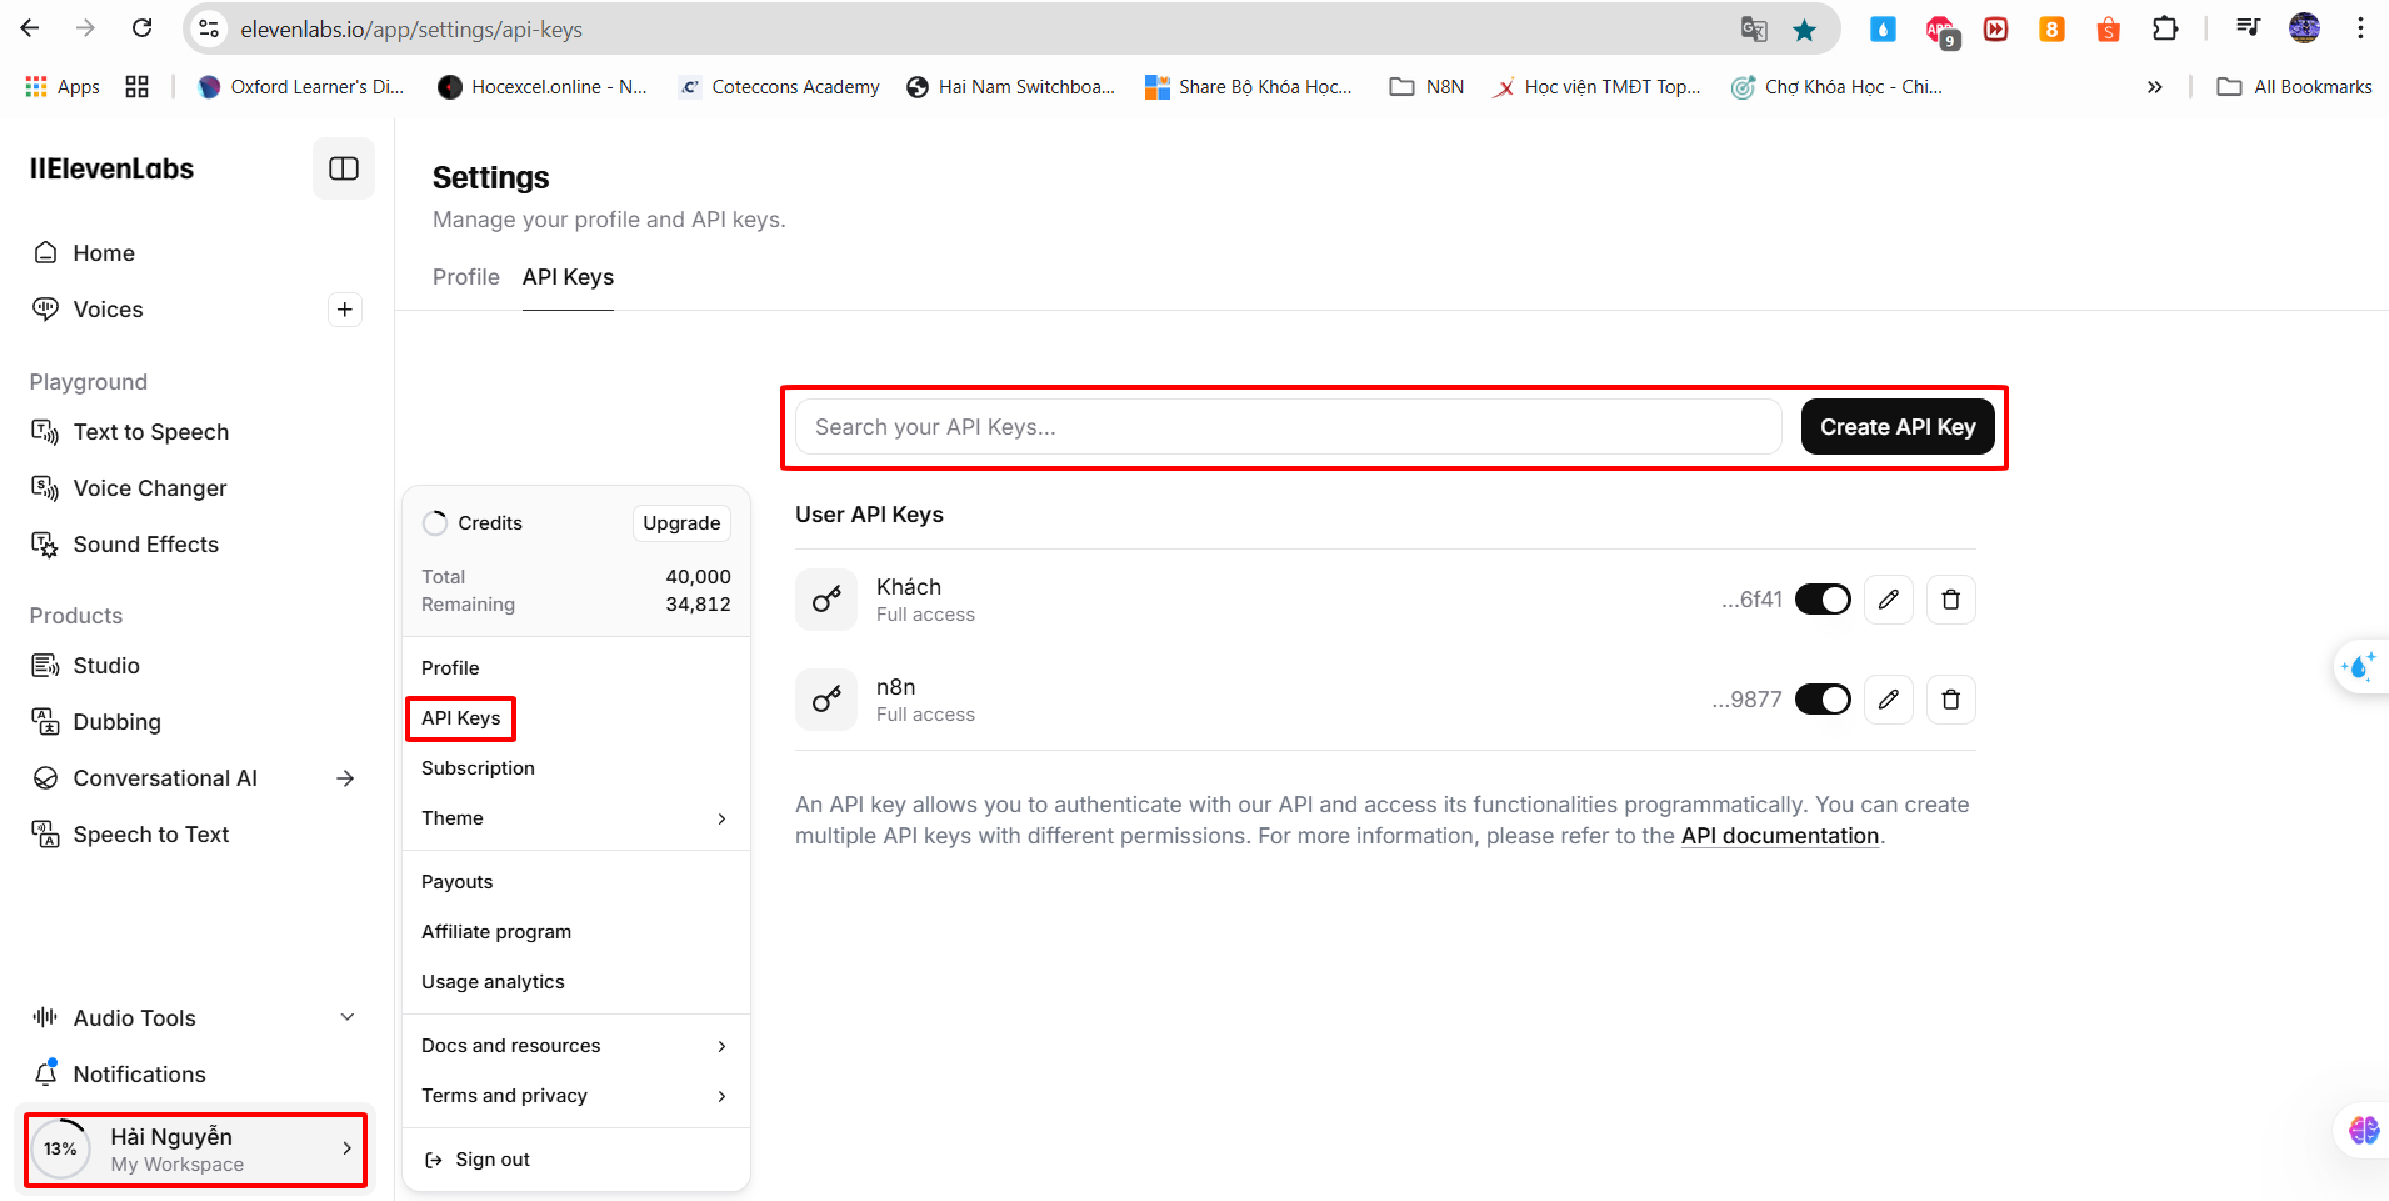
\includegraphics[width=1.0\textwidth]{images/Elevenlabs.pdf}
    \caption{Tạo API Elevenlabs}
    
    \end{figure}
 Tạo được API có dạng " sk\_7529a9c2502bb52789fa8cfcdafdc645c5edc038244e3136 " \\
 
    \begin{figure}[H]
    \centering
    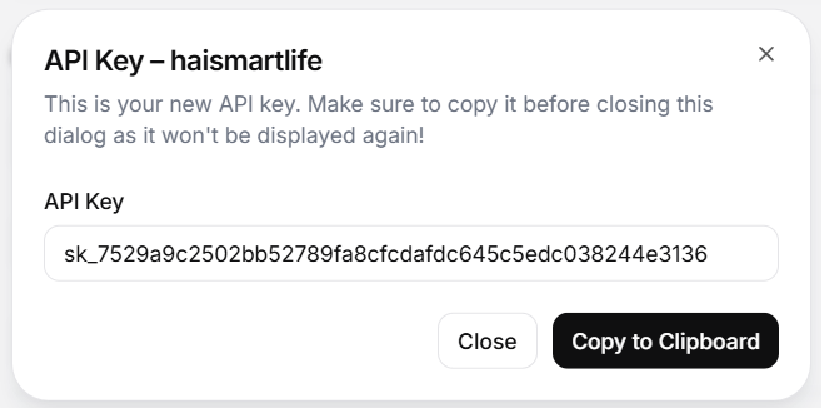
\includegraphics[width=0.6\textwidth]{images/Elevenlabs-1.pdf}
    \caption{Tạo API Elevenlabs}
    
    \end{figure}

    \item \textbf{Bước 2: Tạo node "HTTP truy cập Elevenlabs" trong n8n}\\
    
    \begin{figure}[h]
 
    \centering
    \begin{minipage}{0.45\textwidth}
        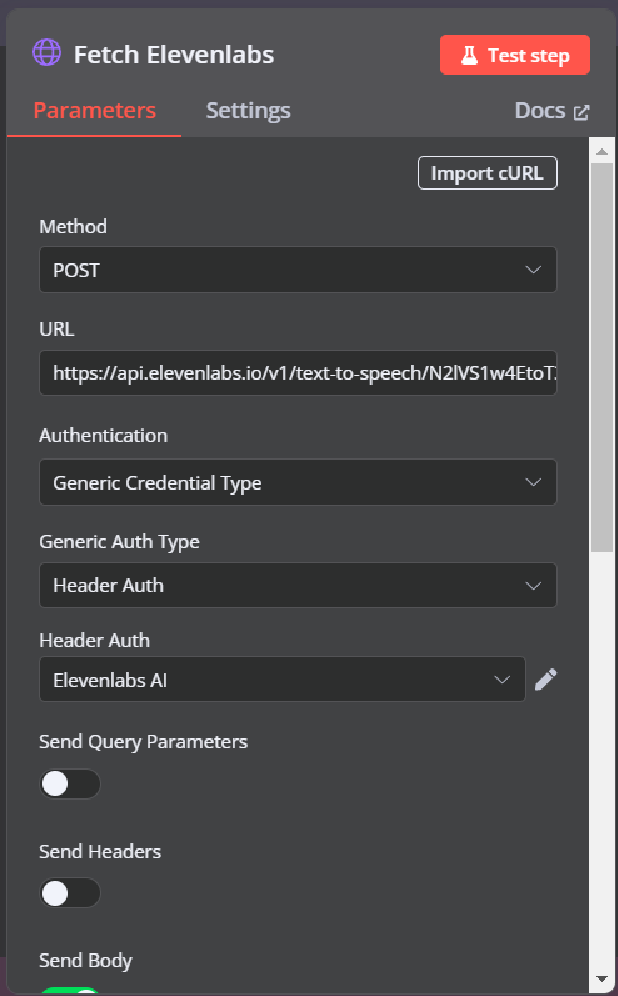
\includegraphics[width=\linewidth]{images/Elevenlabs-2.pdf}
    \end{minipage}
    %\hfill
    \hspace{5pt}
    \begin{minipage}{0.45\textwidth}
         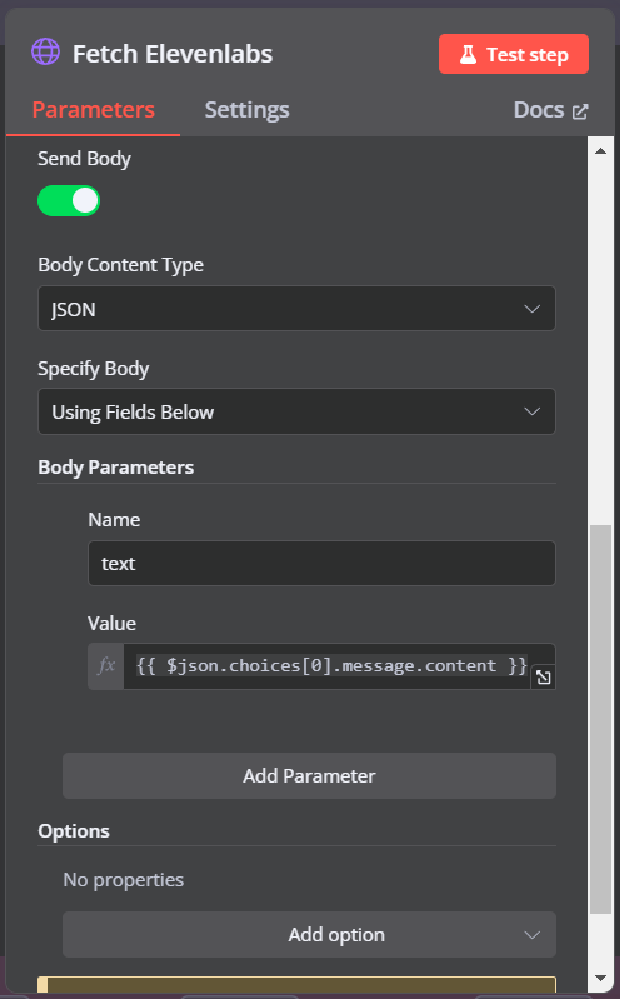
\includegraphics[width=\linewidth]{images/Elevenlabs-3.pdf}
    \end{minipage}
\end{figure}

Tại mục URL nhập: \\
"https://api.elevenlabs.io/v1/text-to-speech/N2lVS1w4EtoT3dr4eOWO"\\

Trong đó "N2lVS1w4EtoT3dr4eOWO" chính là ID của giọng nói mà các bạn muốn xuất hiện trong video

 \begin{figure}[H]
    \centering
    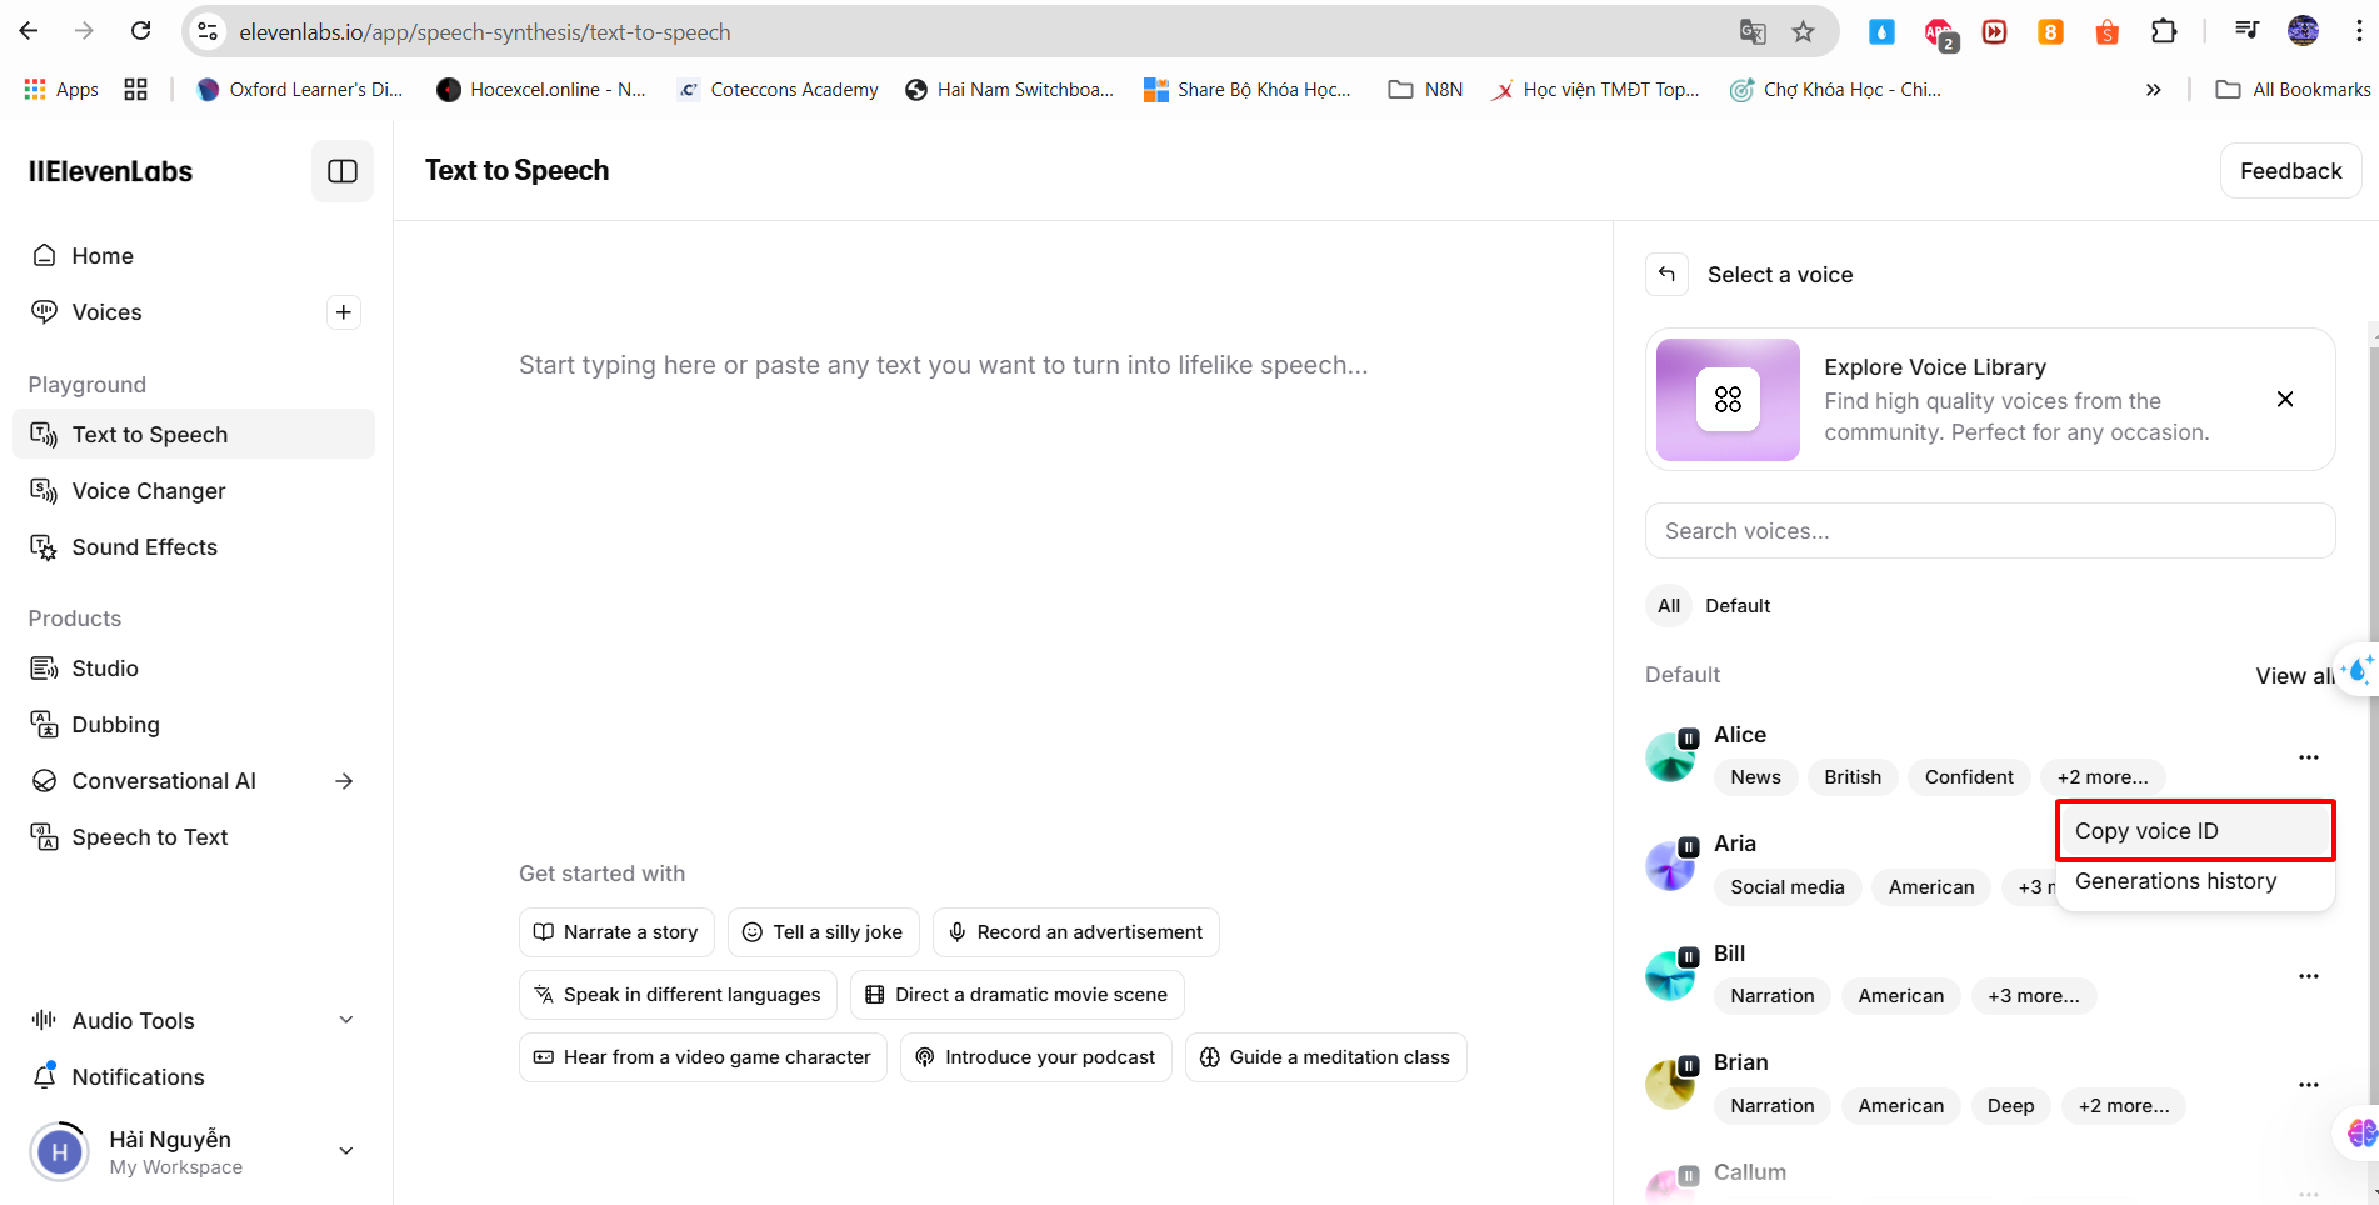
\includegraphics[width=1\textwidth]{images/Elevenlabs-4.pdf}
    \caption{Tạo API Elevenlabs}
    
    \end{figure}

 \begin{figure}[H]
    \centering
    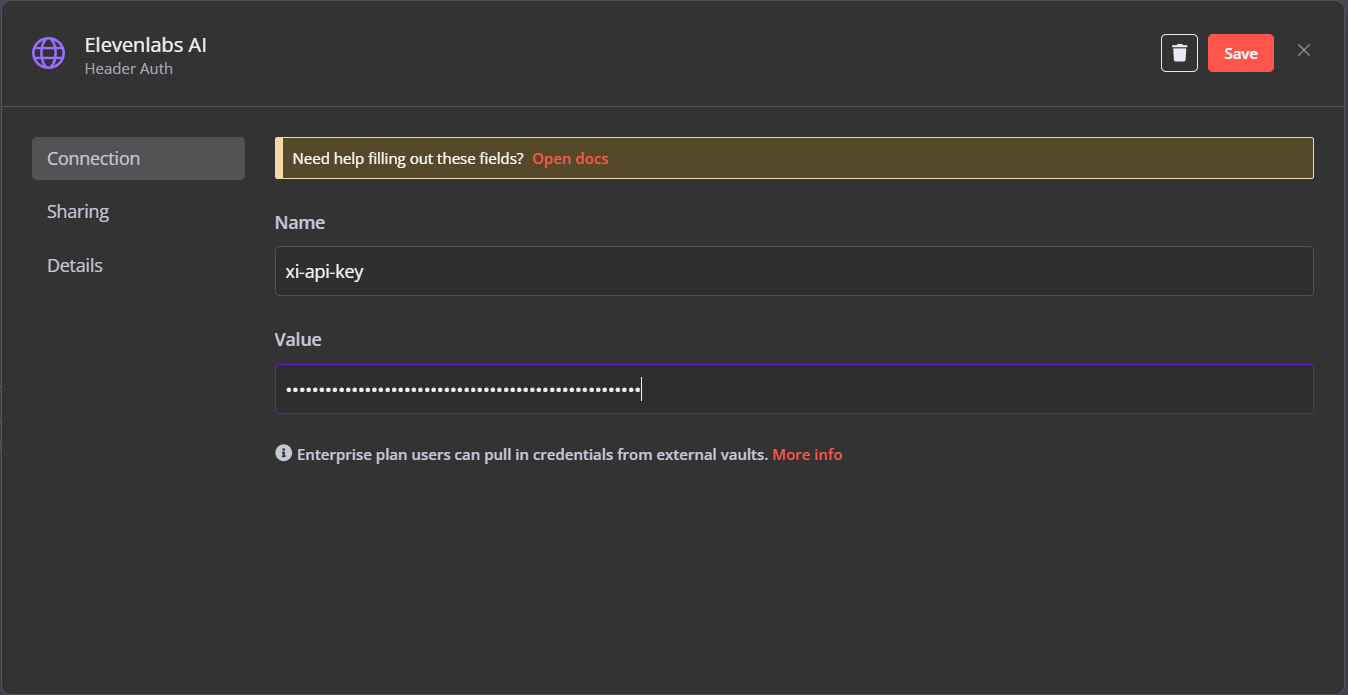
\includegraphics[width=1\textwidth]{images/Elevenlabs-5.png}
    \caption{Tạo API Elevenlabs}
    
    \end{figure}
    Set up credential cho Elevenlabs như hình bên dưới:\\
    Name: xi-api-key\\
    Value: " sk\_7529a9c2502bb52789fa8cfcdafdc645c5edc038244e3136 " (Paste API copy từ web Elevenlabs) \\

\end{itemize}

%--------------------------------------------------------------

\subsection{Together AI - nền tảng hỗ trợ các module AI tối ưu kết quả.}
\begin{itemize}[label=]
    \item \textbf{Bước 1: Tạo API key Together AI} 
    
    Truy cập vào link \url{https://api.together.ai/settings/api-keys} \\ 
    Tìm đến API keys và copy nó ta sẽ được dãy ký tự.\\
    Lưu ý: Thêm thông tin thẻ thanh toán và sử dụng như thường, và có thể thay node này bằng node khác có chức năng tương đương thể thử.\\
    
    \begin{figure}[H]
    \centering
    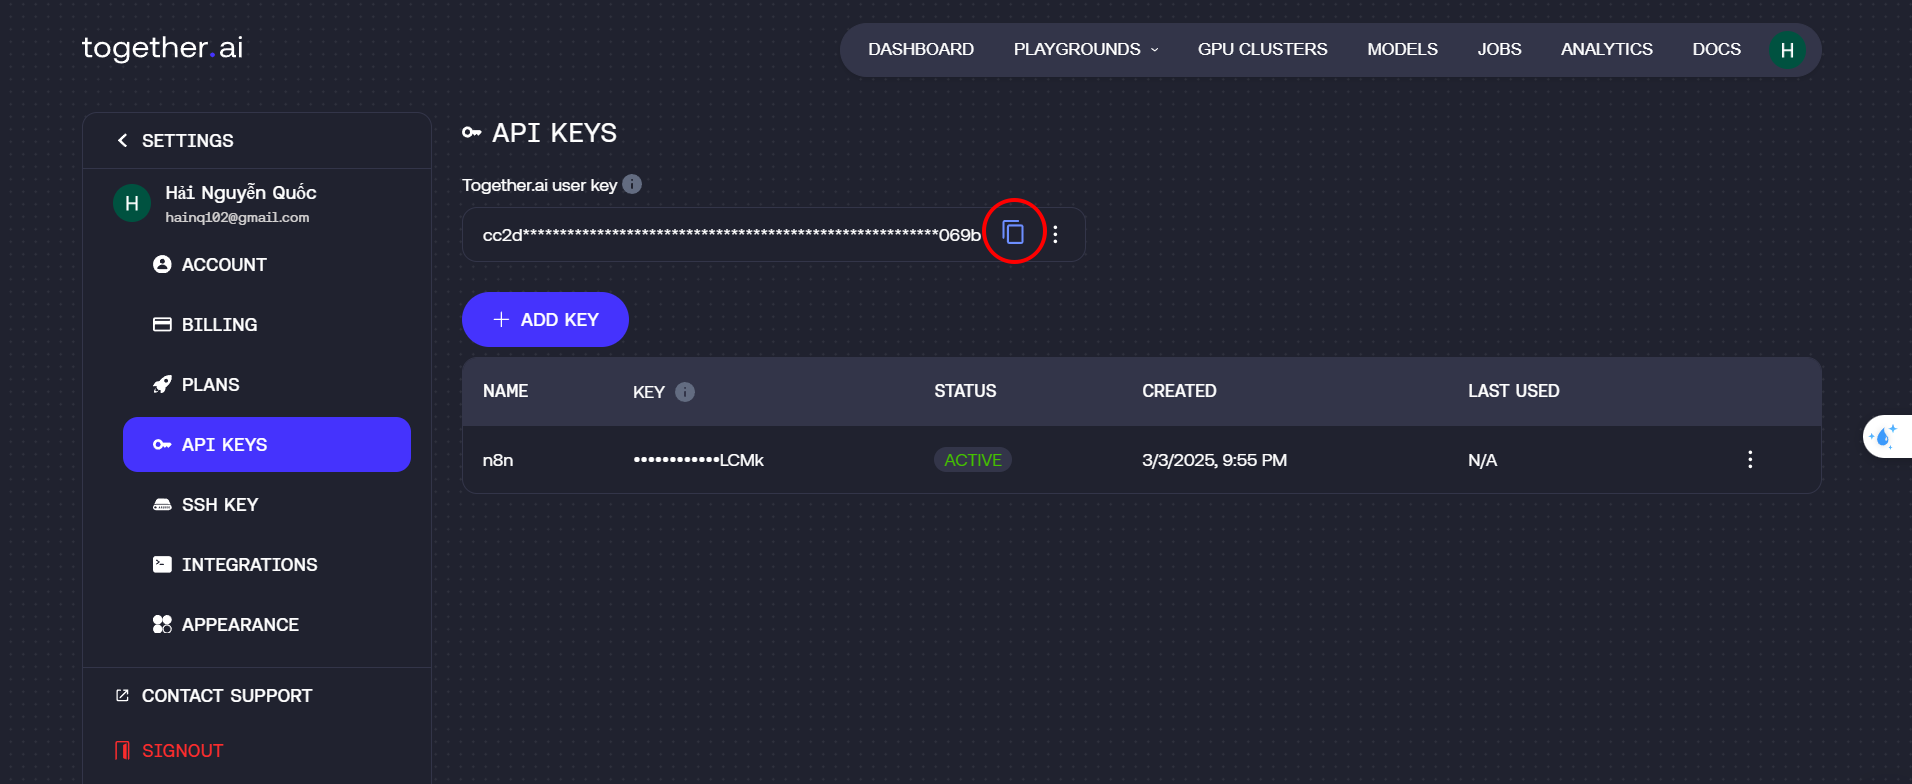
\includegraphics[width=0.95\textwidth]{images/TogetherAI.png}
    \caption{Tạo API Together AI}
    
    \end{figure}
    \item \textbf{Bước 2: Tạo node "HTTP truy cập Together AI" trong n8n}\\
    \begin{figure}[H]
    \centering
    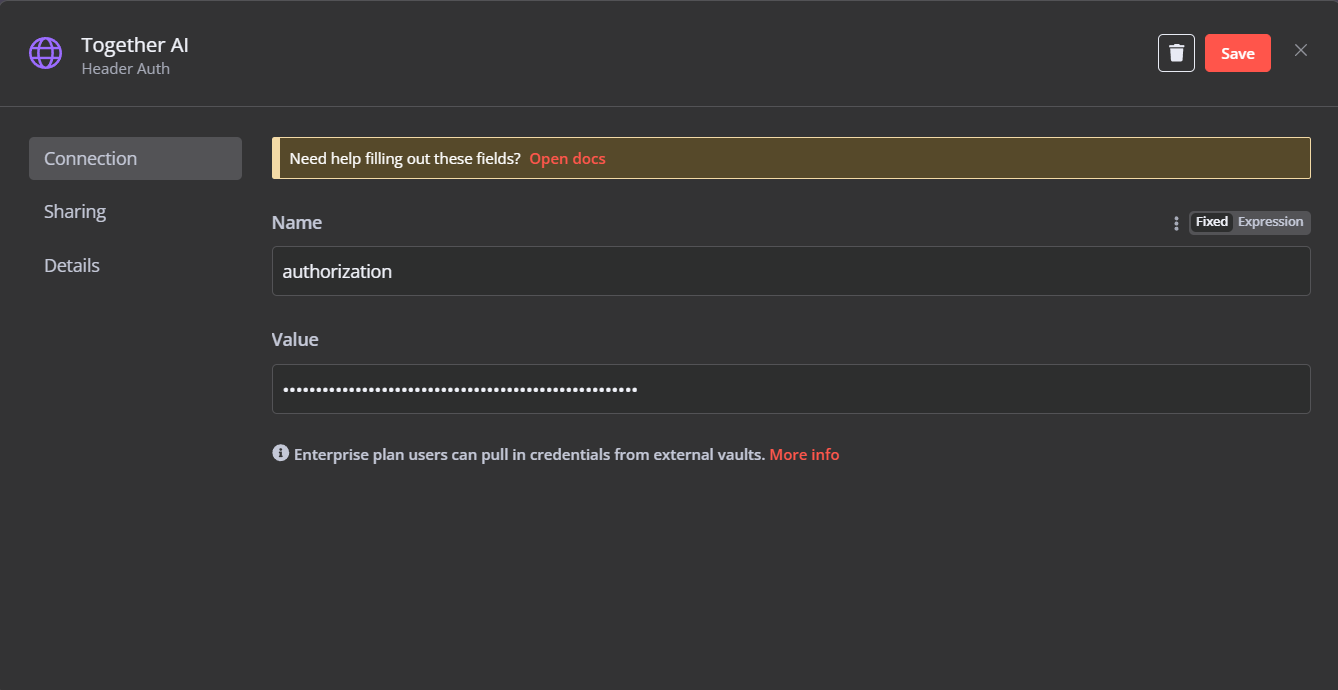
\includegraphics[width=0.95\textwidth]{images/TogetherAI-1.png}
    \caption{Tạo API Elevenlabs}
    
    \end{figure}
    
 Tạo Node HTTP trong n8n, trong phần Header Auth chúng ta tạo credential như hình trên:\\
 Name: authorization\\
 Value: API vừa copy ở web Together AI\\
 
    \begin{figure}[H]
    \centering
    \begin{minipage}{0.45\textwidth}
        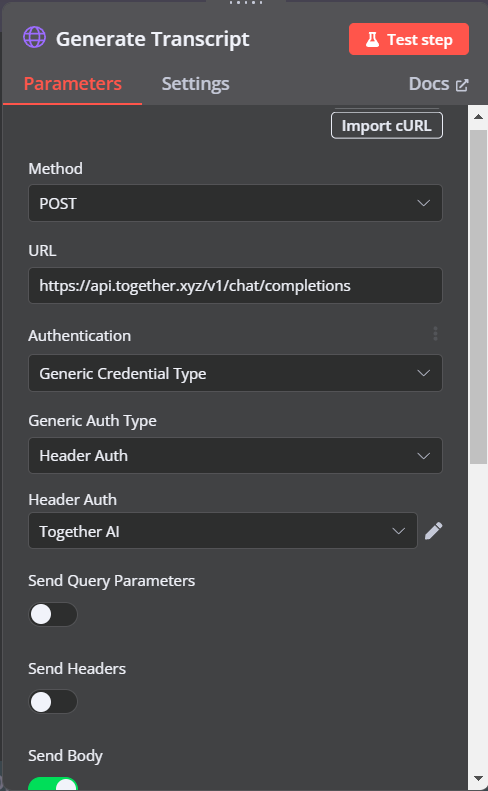
\includegraphics[width=\linewidth]{images/TogetherAI-2.png}
    \end{minipage}
    %\hfill
    \hspace{5pt}
    \begin{minipage}{0.45\textwidth}
         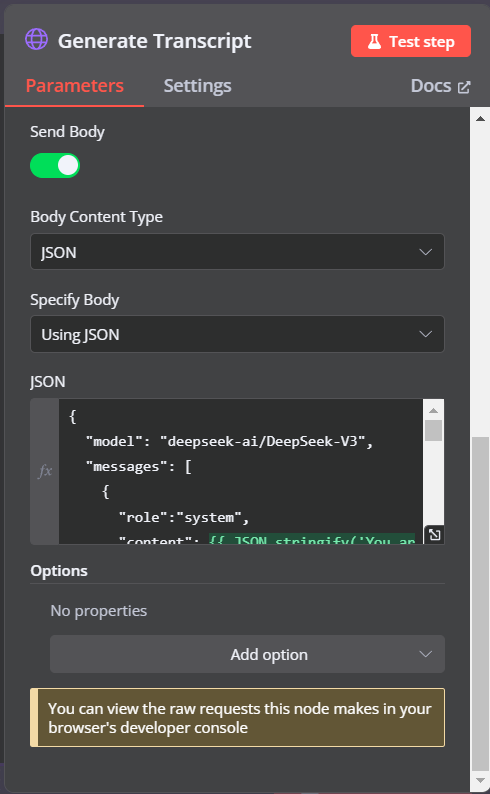
\includegraphics[width=\linewidth]{images/TogetherAI-3.png}
    \end{minipage}
\end{figure}

Tại mục URL nhập: \\
"https://api.together.xyz/v1/chat/completions"\\

Tại mục Json nhập: 


Dưới đây là đoạn JSON:\\

Nơi lấy code \url{https://haismartlife.com/}


\end{itemize}

%------------------------------------------------------
\subsection{Google cloud storage - Lưu trữ các video, Audio, Hình ảnh tạo ra}
\begin{itemize}[label=]
    \item \textbf{Bước 1: Set up tài khoản} 
    
    Truy cập vào link \url{https://console.cloud.google.com/} \\ 

    \begin{figure}[H]
    \centering
    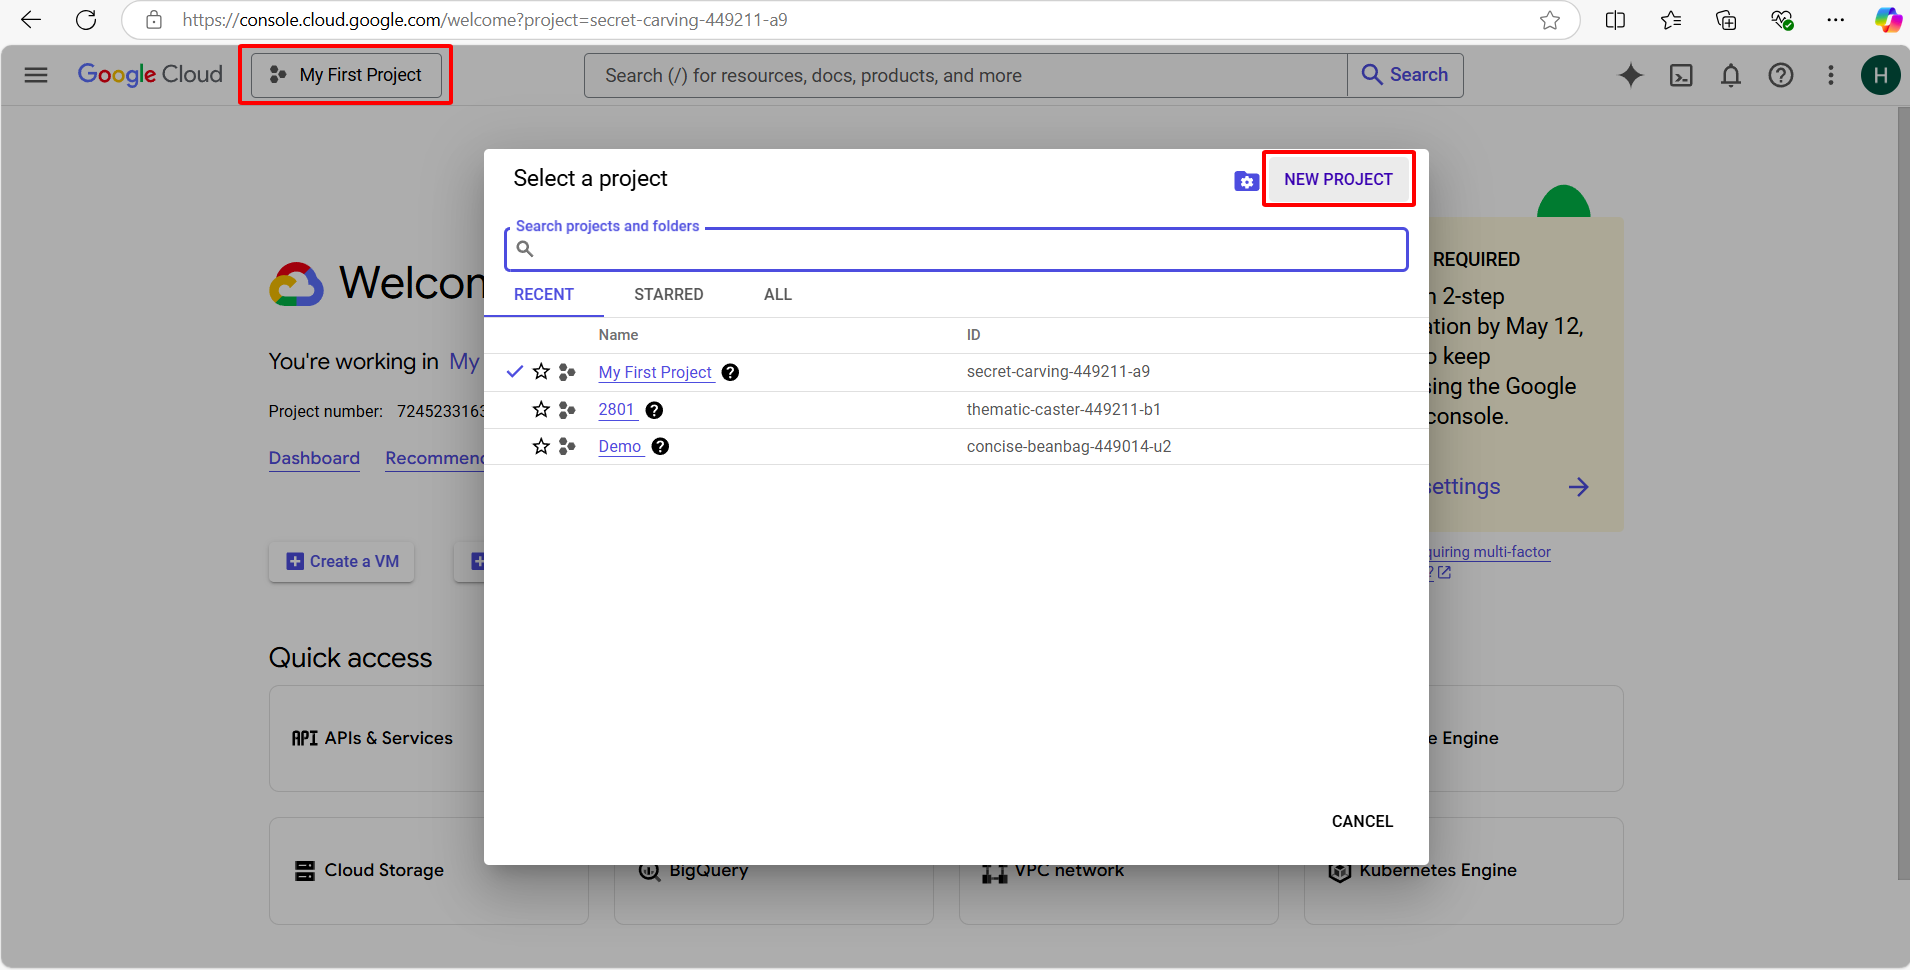
\includegraphics[width=0.95\textwidth]{images/GGcloud.png}
    \caption{Tạo API Together AI}
    
    \end{figure}
    \begin{figure}[H]
    \centering
    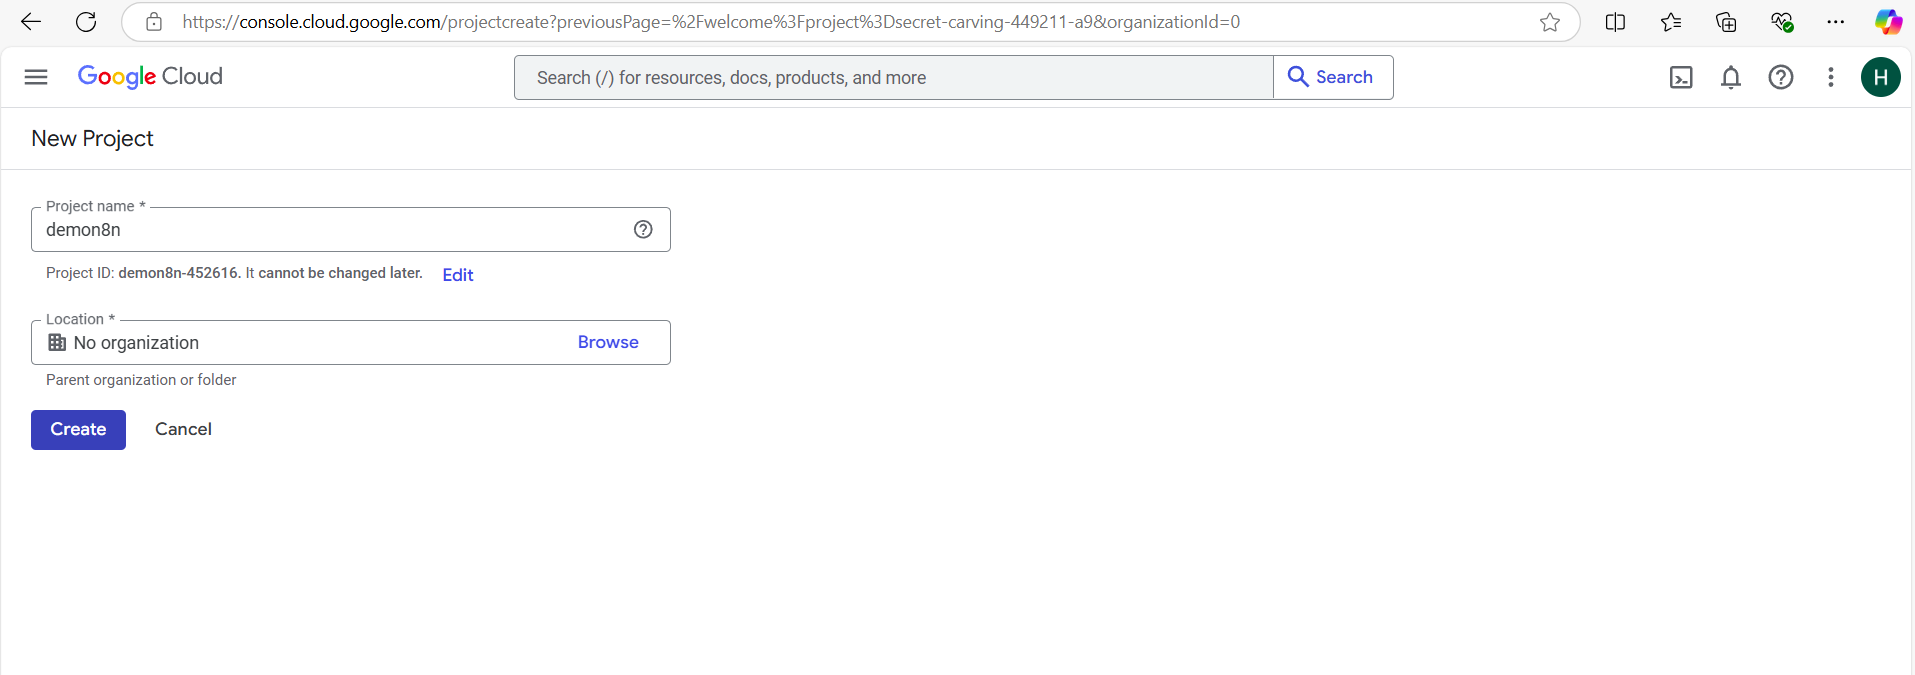
\includegraphics[width=0.95\textwidth]{images/GGcloud-1.png}
    \caption{Tạo API Together AI}
    
    \end{figure}
    
    \begin{figure}[H]
    \centering
    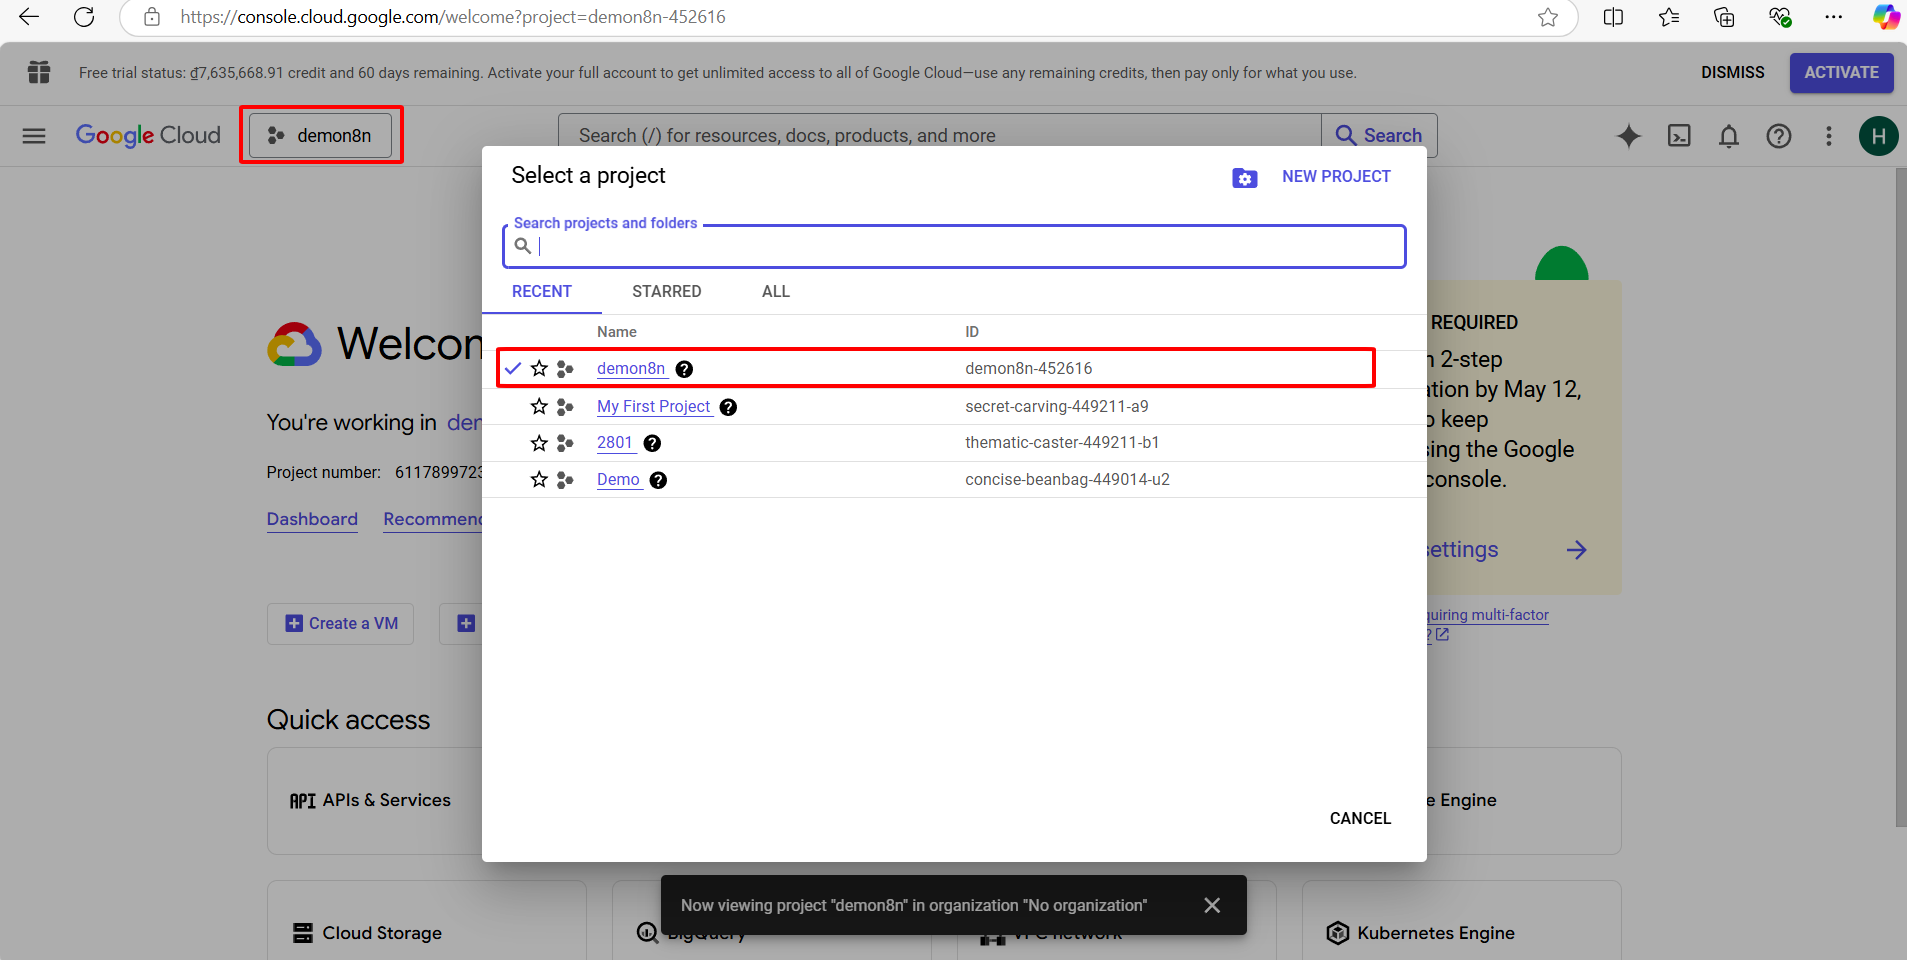
\includegraphics[width=0.95\textwidth]{images/GGcloud-2.png}
    \caption{Tạo API Together AI}
    
    \end{figure}
    \begin{figure}[H]
    \centering
    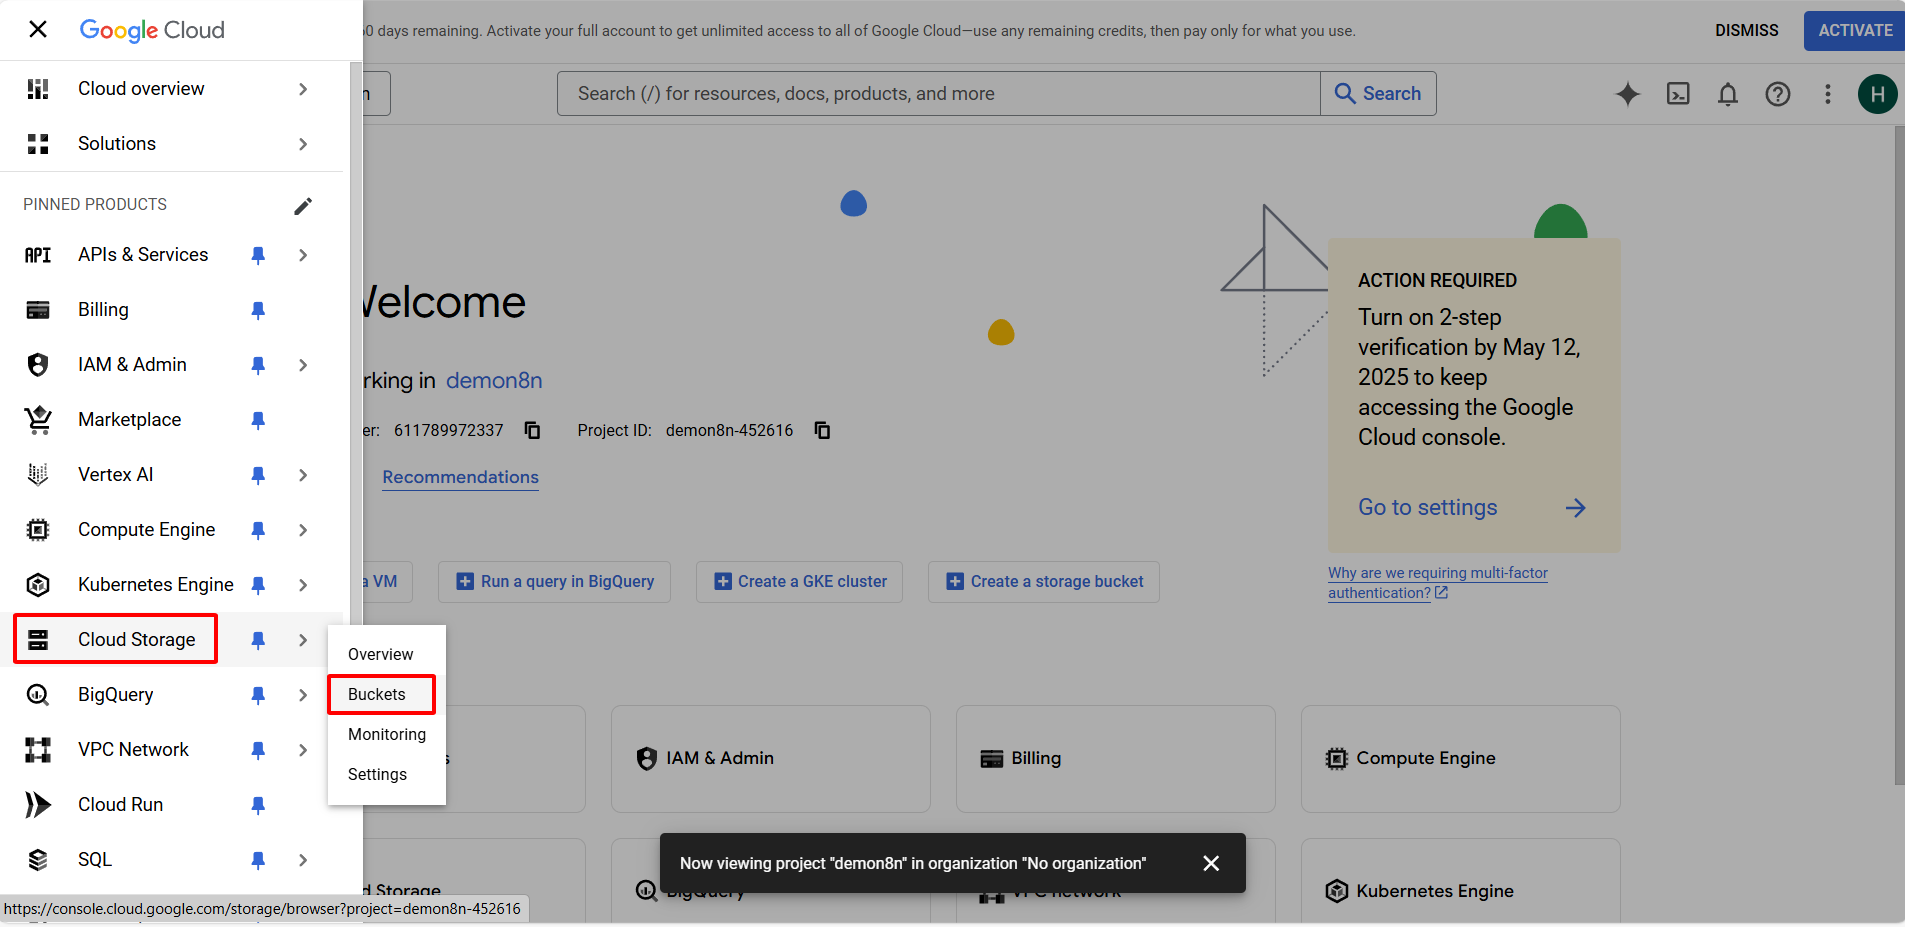
\includegraphics[width=0.95\textwidth]{images/GGcloud-3.png}
    \caption{Tạo API Together AI}
    
    \end{figure}
    \begin{figure}[H]
    \centering
    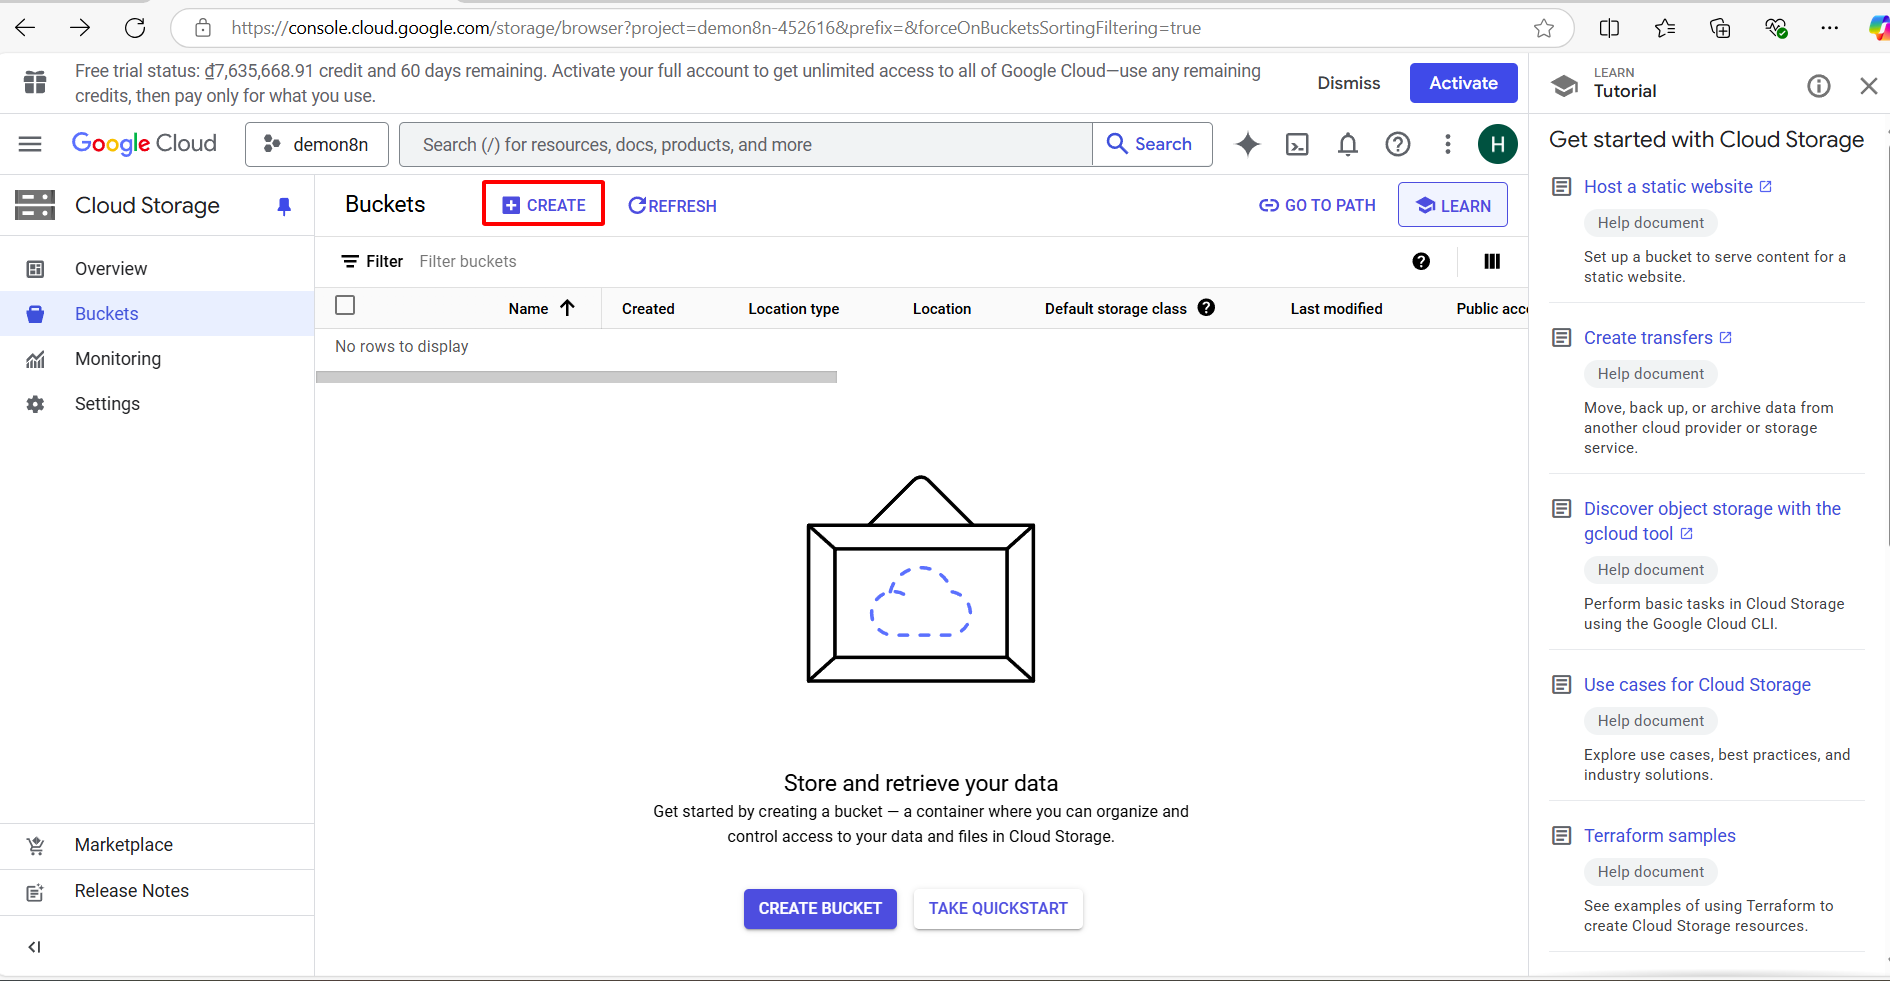
\includegraphics[width=0.95\textwidth]{images/GGcloud-4.png}
    \caption{Tạo API Together AI}
    
    \end{figure}
    \begin{figure}[H]
    \centering
    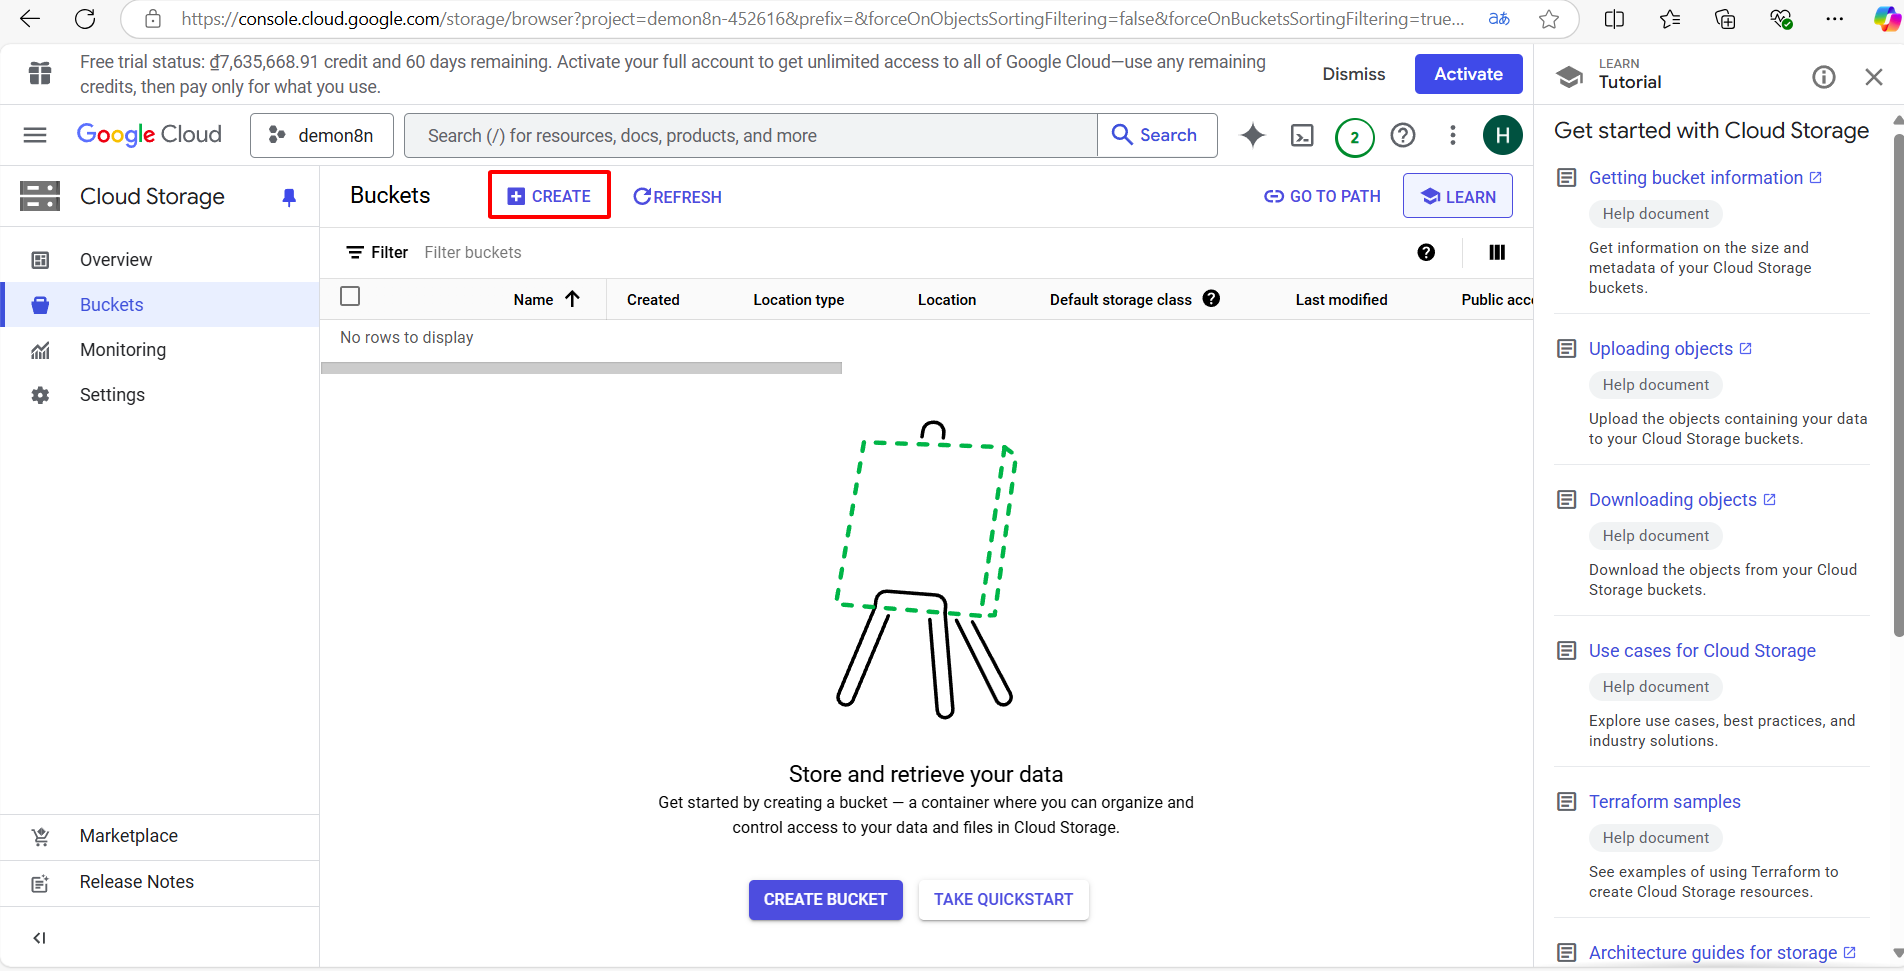
\includegraphics[width=0.95\textwidth]{images/GGcloud-5.png}
    \caption{Tạo API Together AI}
    
    \end{figure}
    \begin{figure}[H]
    \centering
    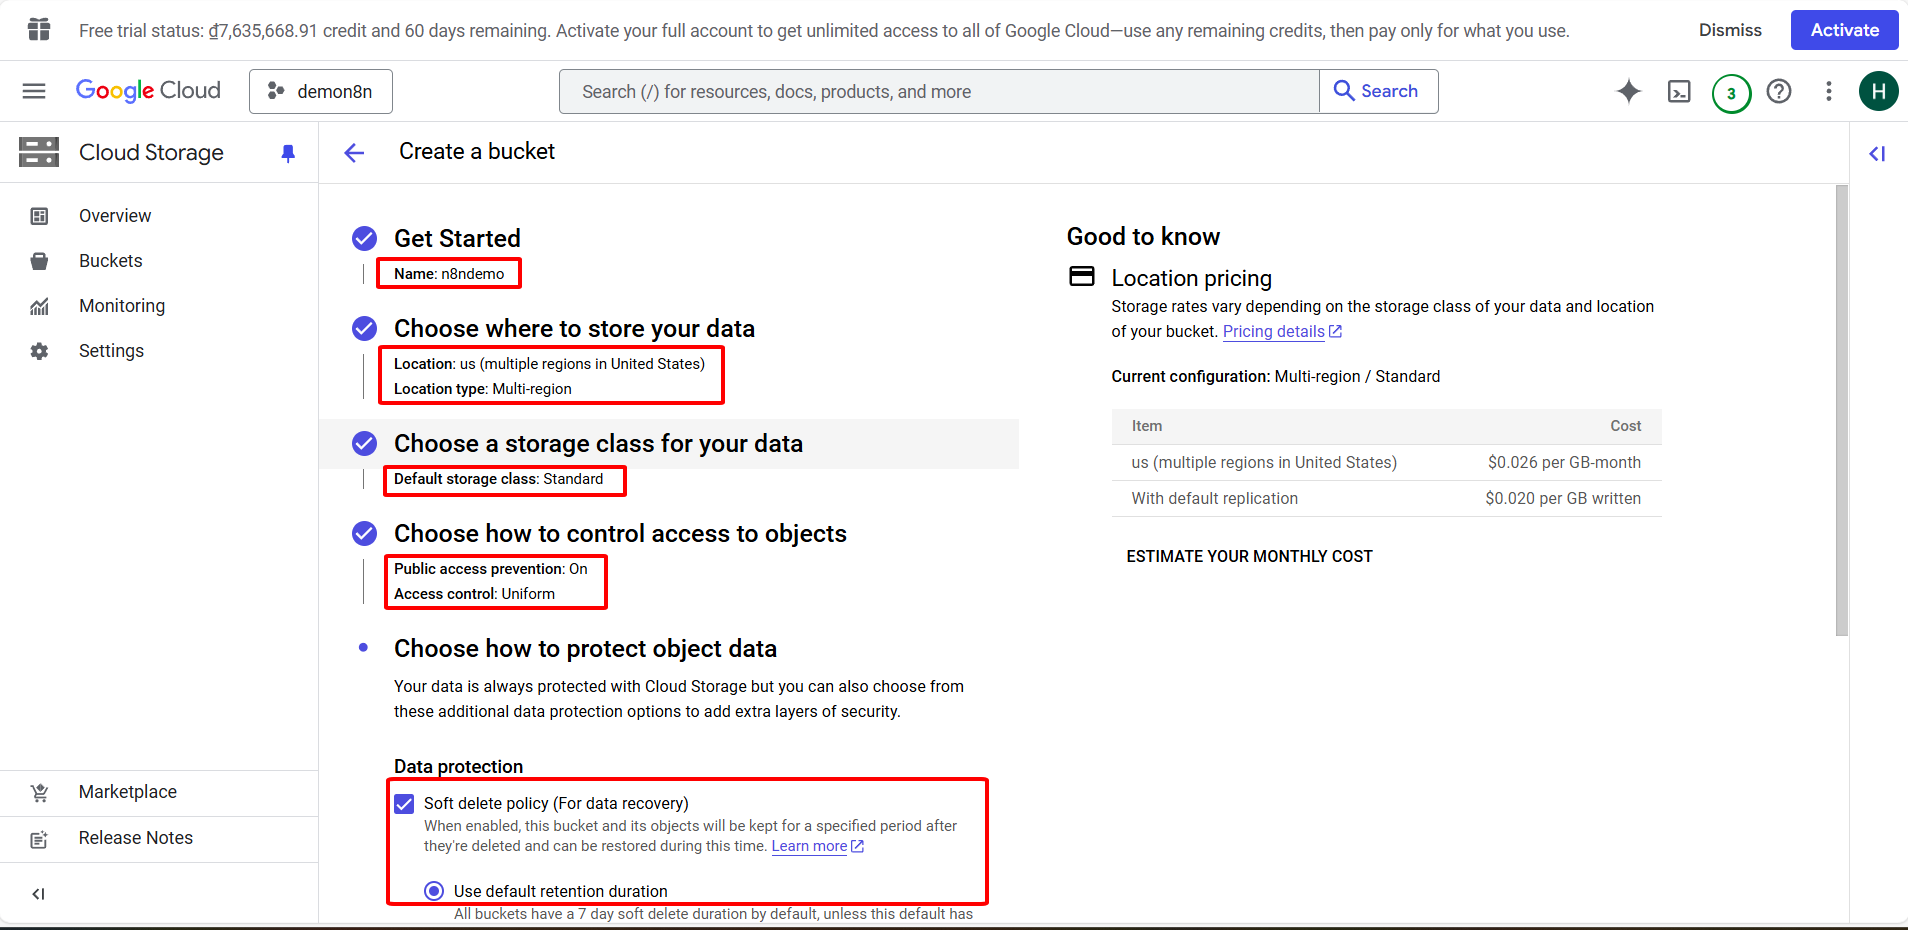
\includegraphics[width=0.95\textwidth]{images/GGcloud-6.png}
    \caption{Tạo API Together AI}
    
    \end{figure}
    \begin{figure}[H]
    \centering
    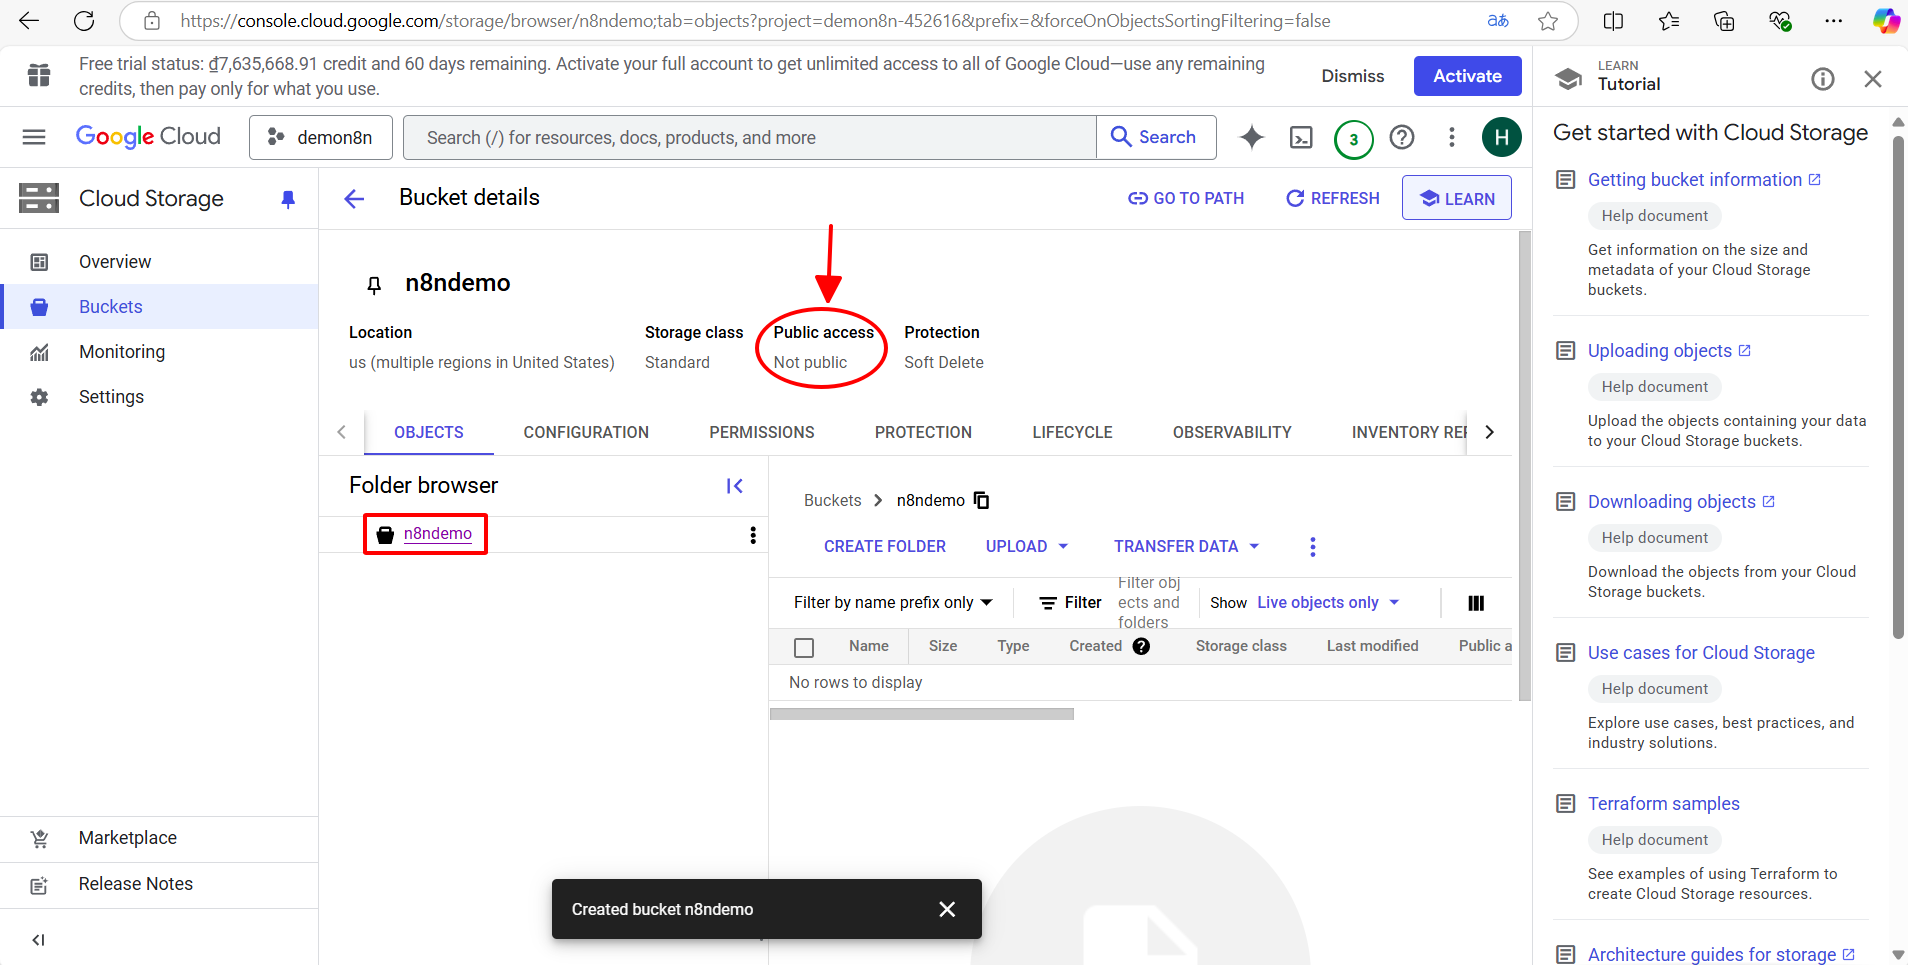
\includegraphics[width=0.95\textwidth]{images/GGcloud-7.png}
    \caption{Tạo API Together AI}
    
    \end{figure}
    \begin{figure}[H]
    \centering
    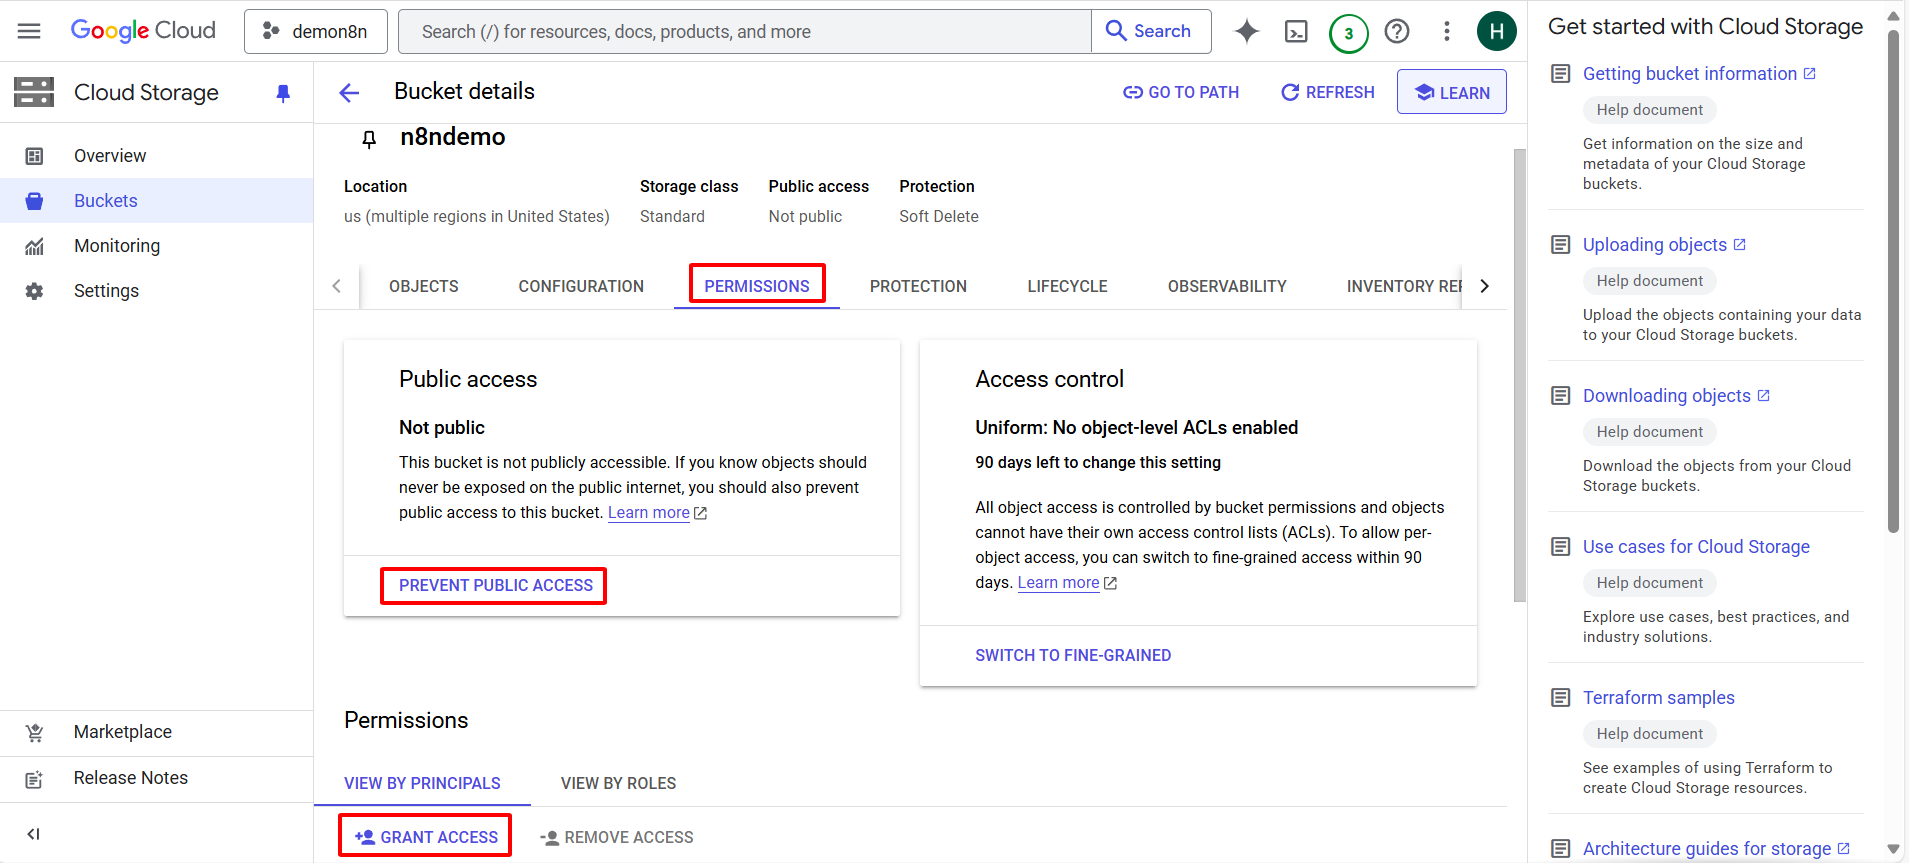
\includegraphics[width=0.95\textwidth]{images/GGcloud-8.png}
    \caption{Tạo API Together AI}
    
    \end{figure}
    \begin{figure}[H]
    \centering
    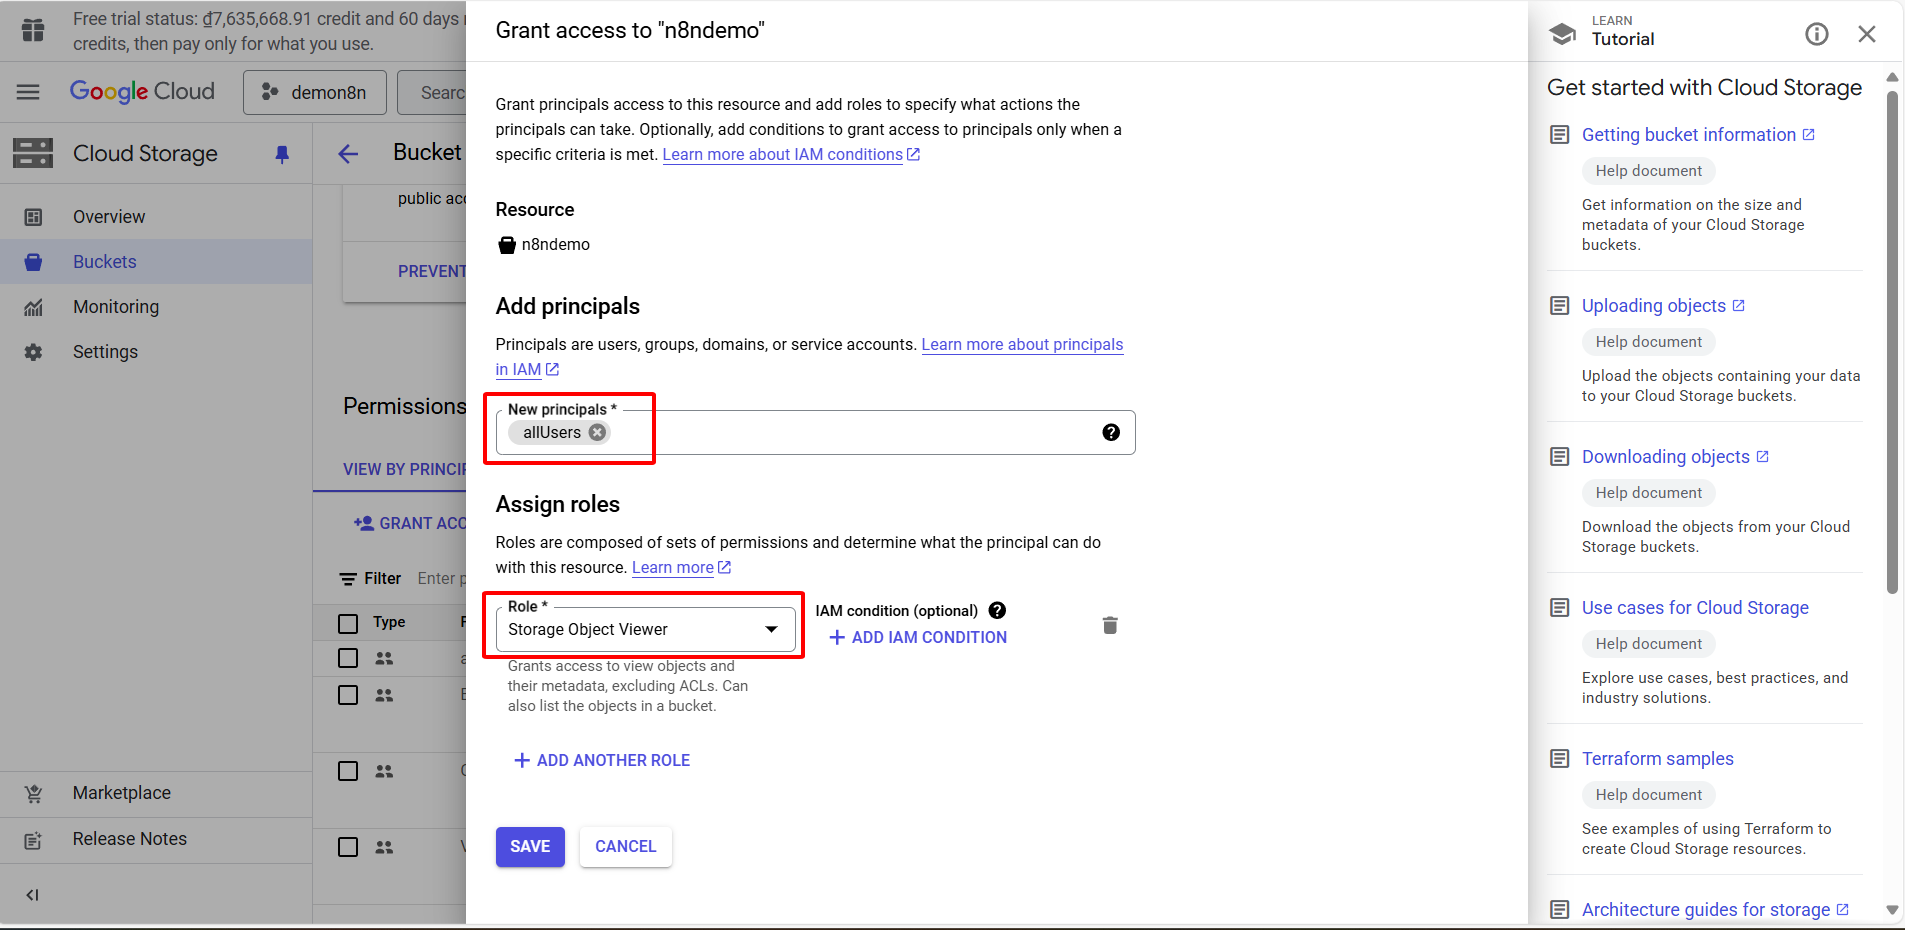
\includegraphics[width=0.95\textwidth]{images/GGcloud-9.png}
    \caption{Tạo API Together AI}
    
    \end{figure}
    \begin{figure}[H]
    \centering
    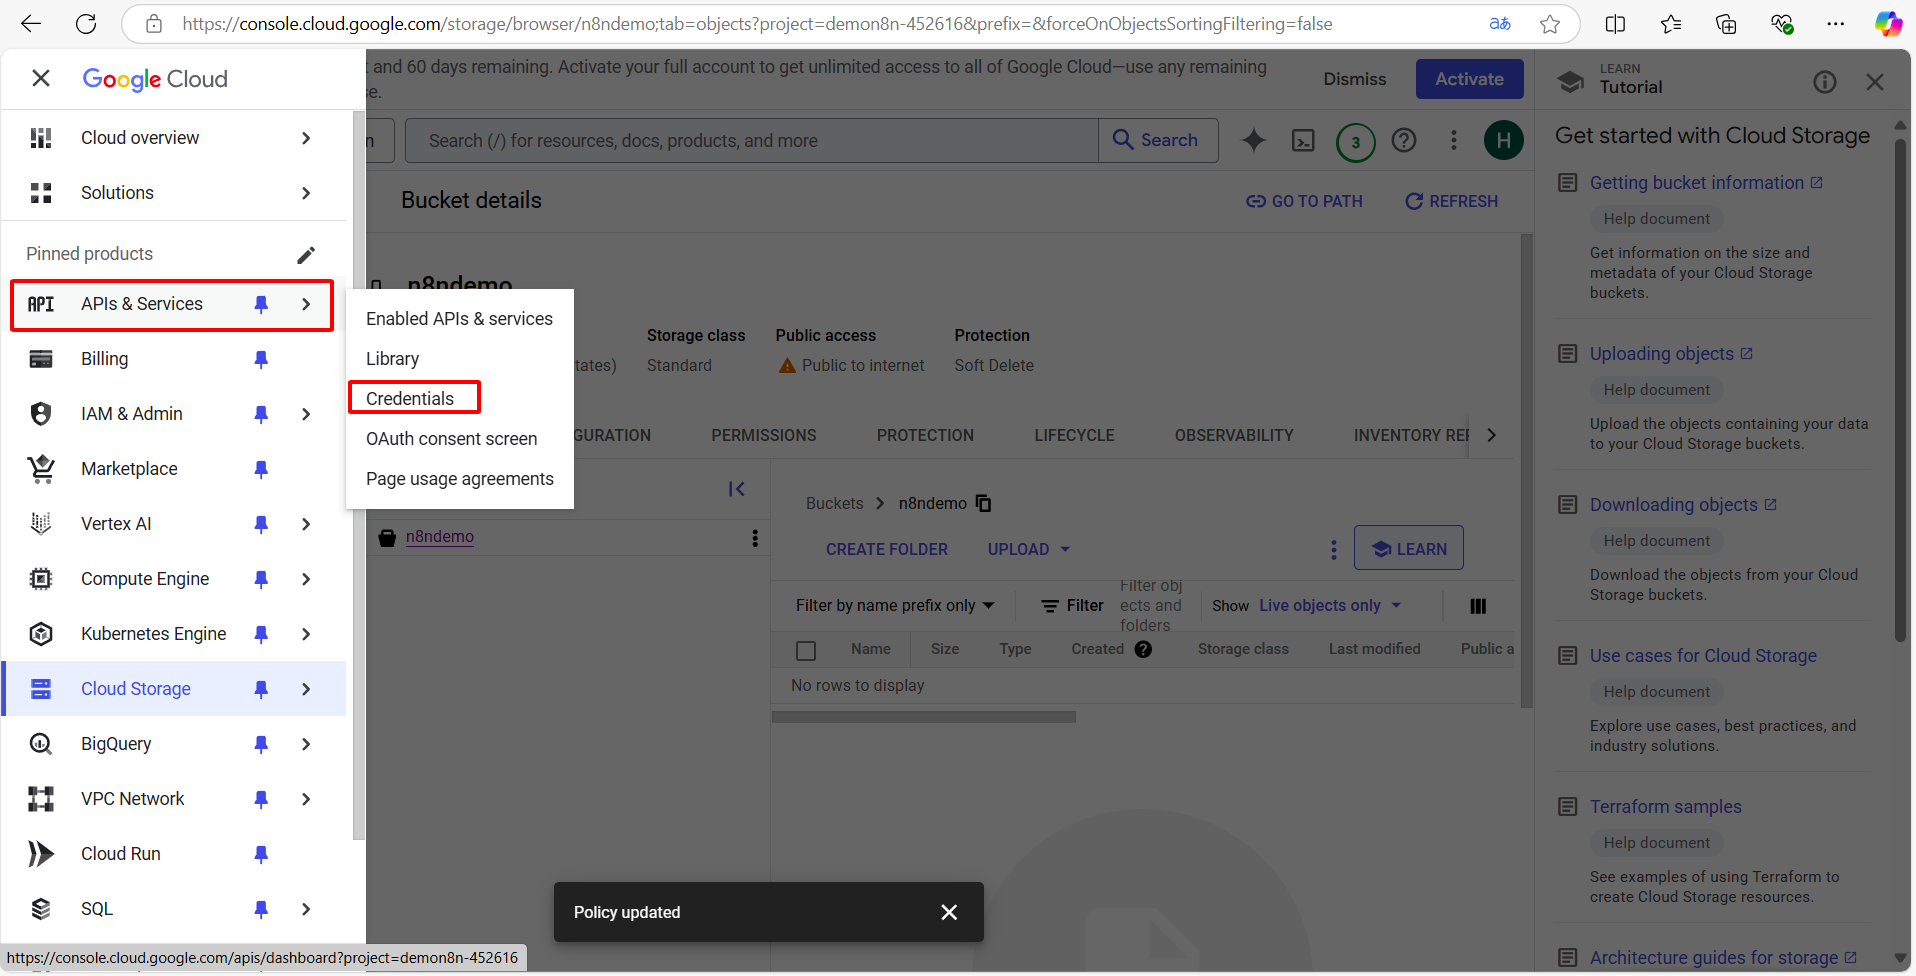
\includegraphics[width=0.95\textwidth]{images/GGcloud-10.png}
    \caption{Tạo API Together AI}
    
    \end{figure}
        \begin{figure}[H]
    \centering
    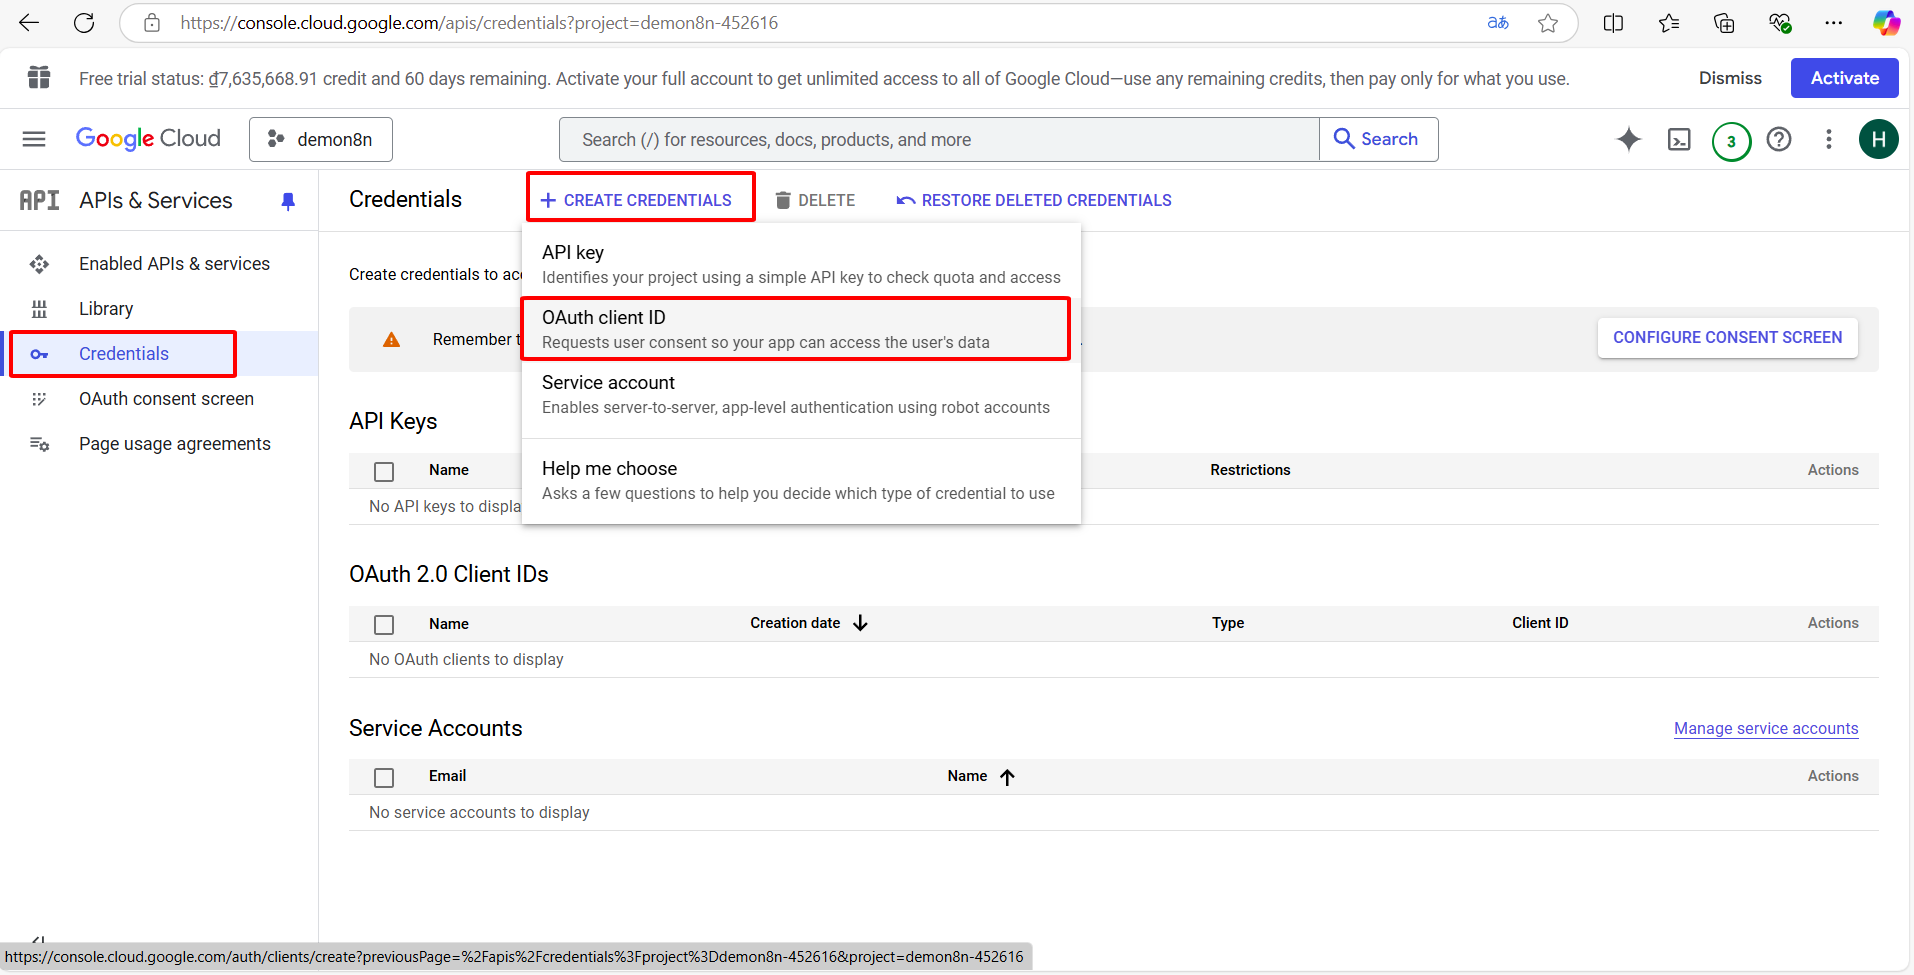
\includegraphics[width=0.95\textwidth]{images/GGcloud-11.png}
    \caption{Tạo API Together AI}
    
    \end{figure}
    \begin{figure}[H]
    \centering
    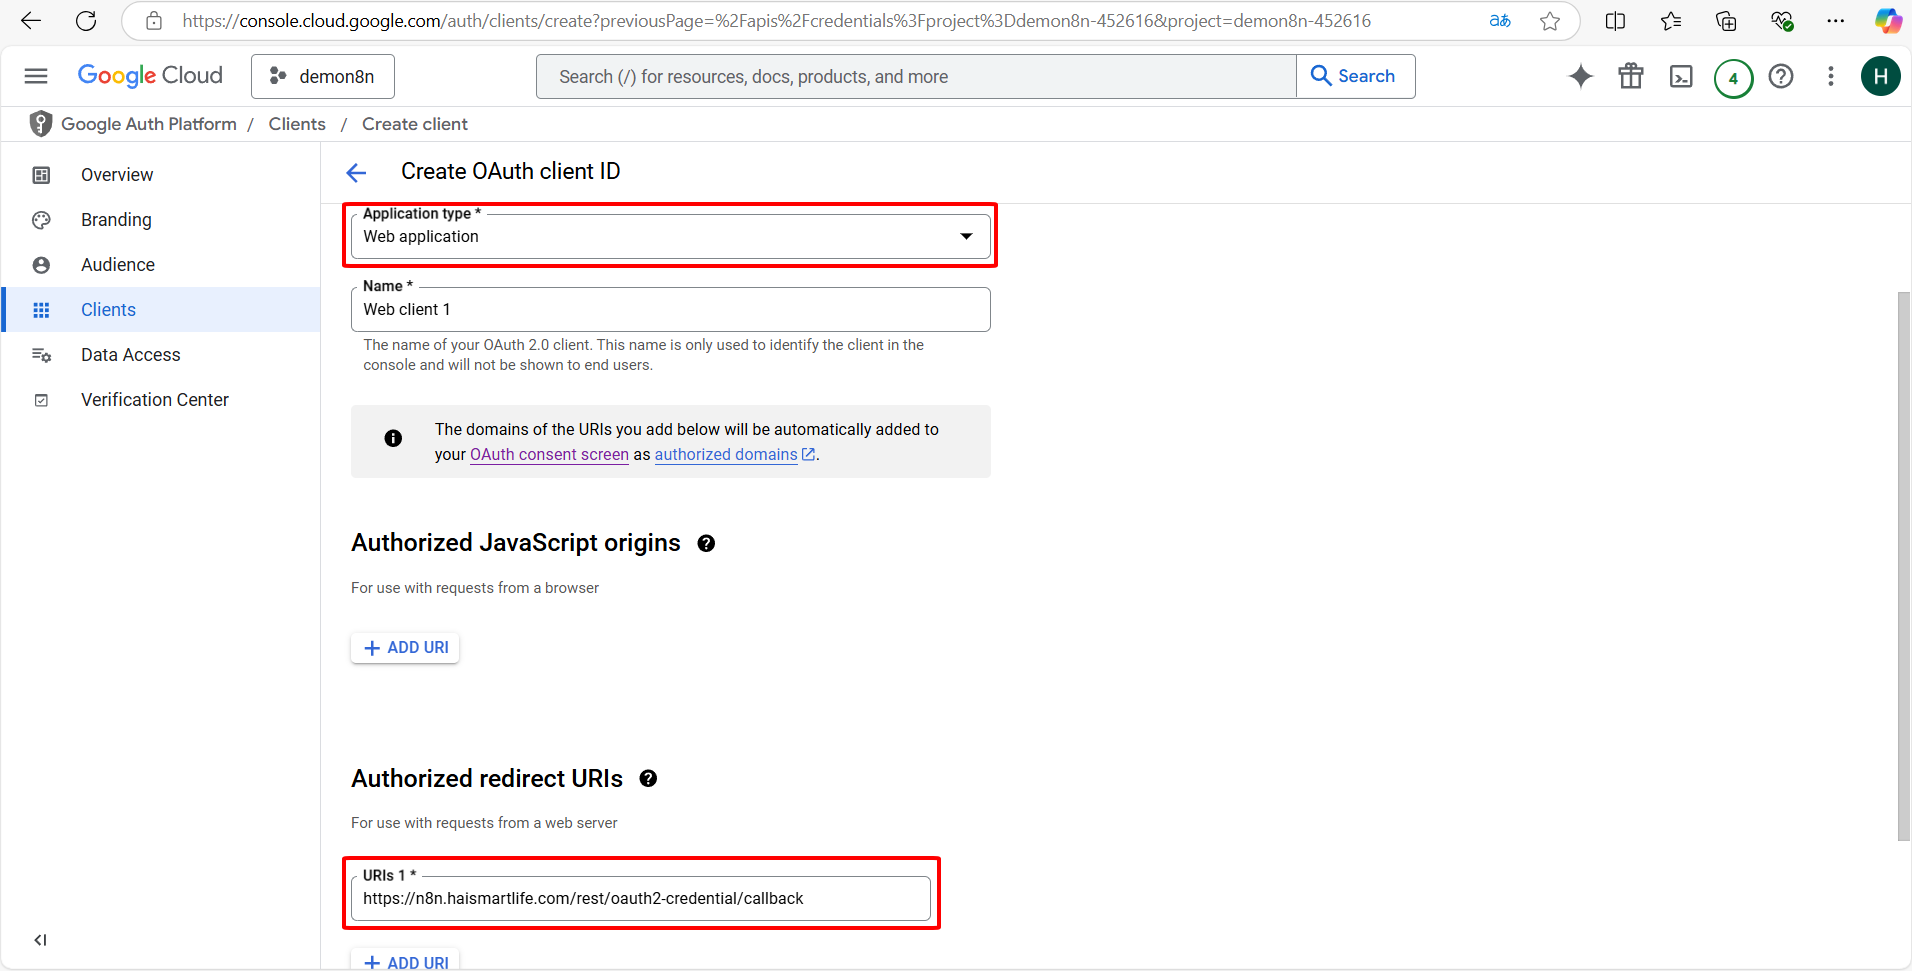
\includegraphics[width=0.95\textwidth]{images/GGcloud-12.png}
    \caption{Tạo API Together AI}
    
    \end{figure}

    \begin{figure}[H]
    \centering
    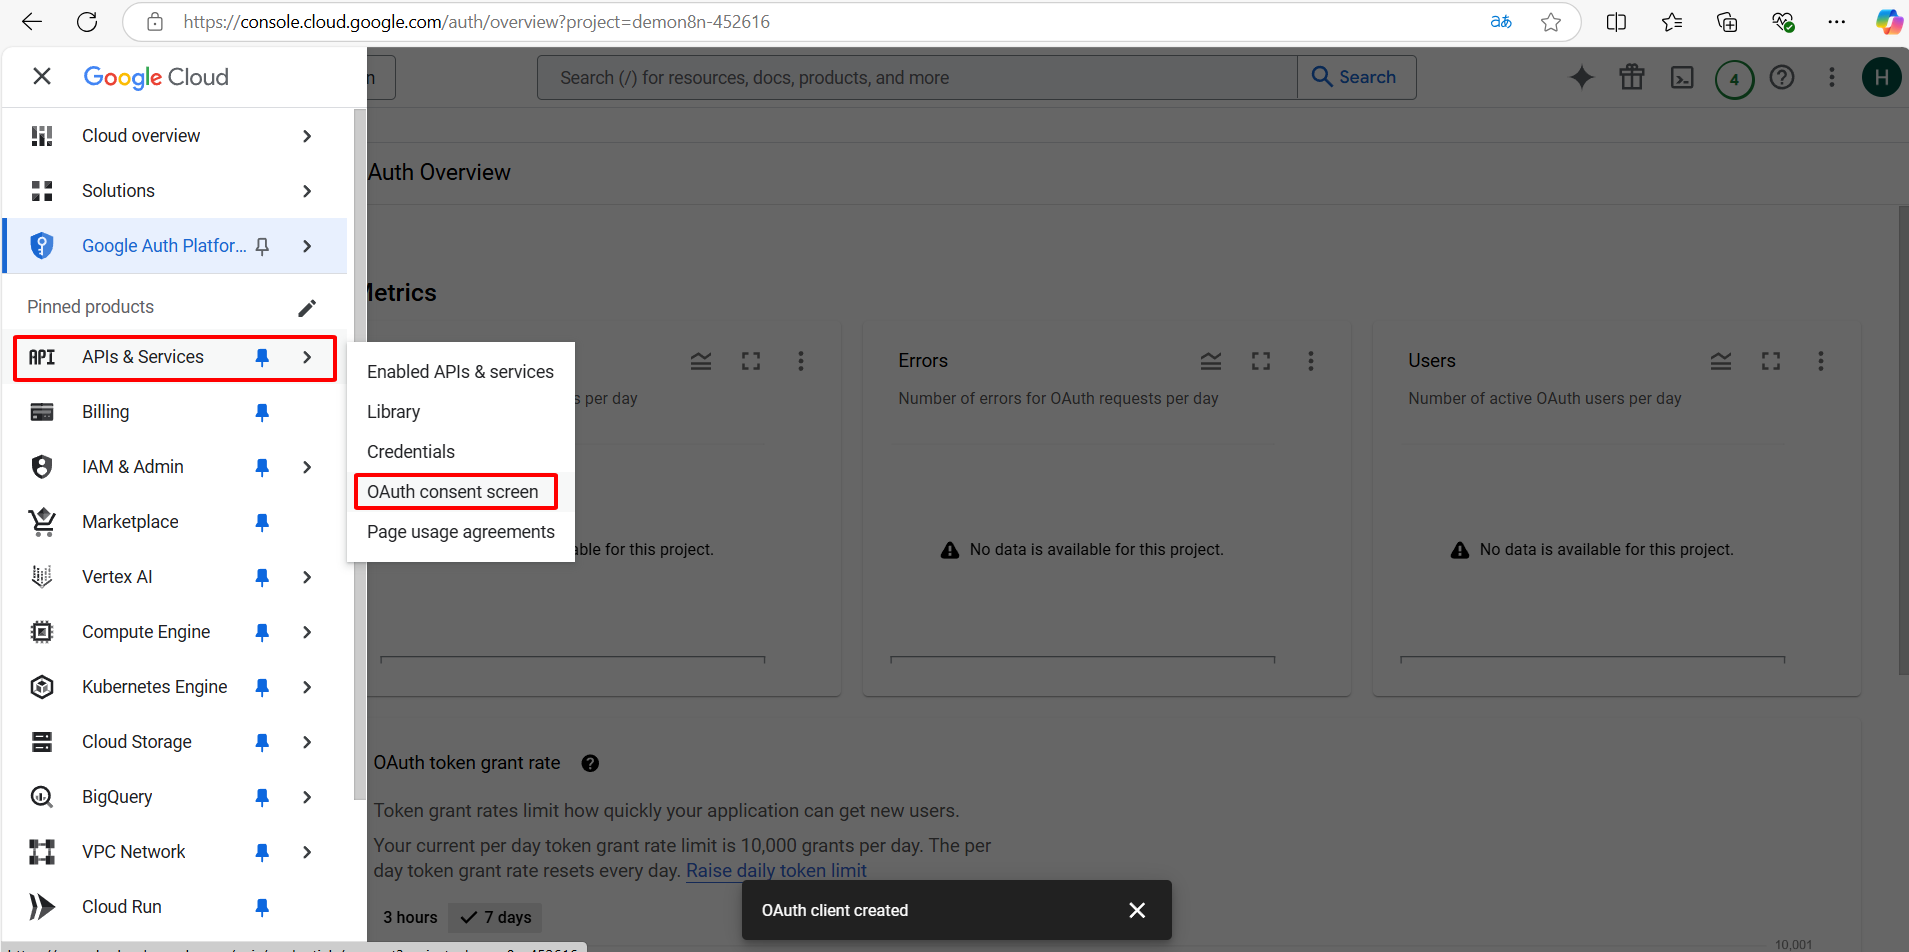
\includegraphics[width=0.95\textwidth]{images/GGcloud-14.png}
    \caption{Tạo API Together AI}
    
    \end{figure}
    \begin{figure}[H]
    \centering
    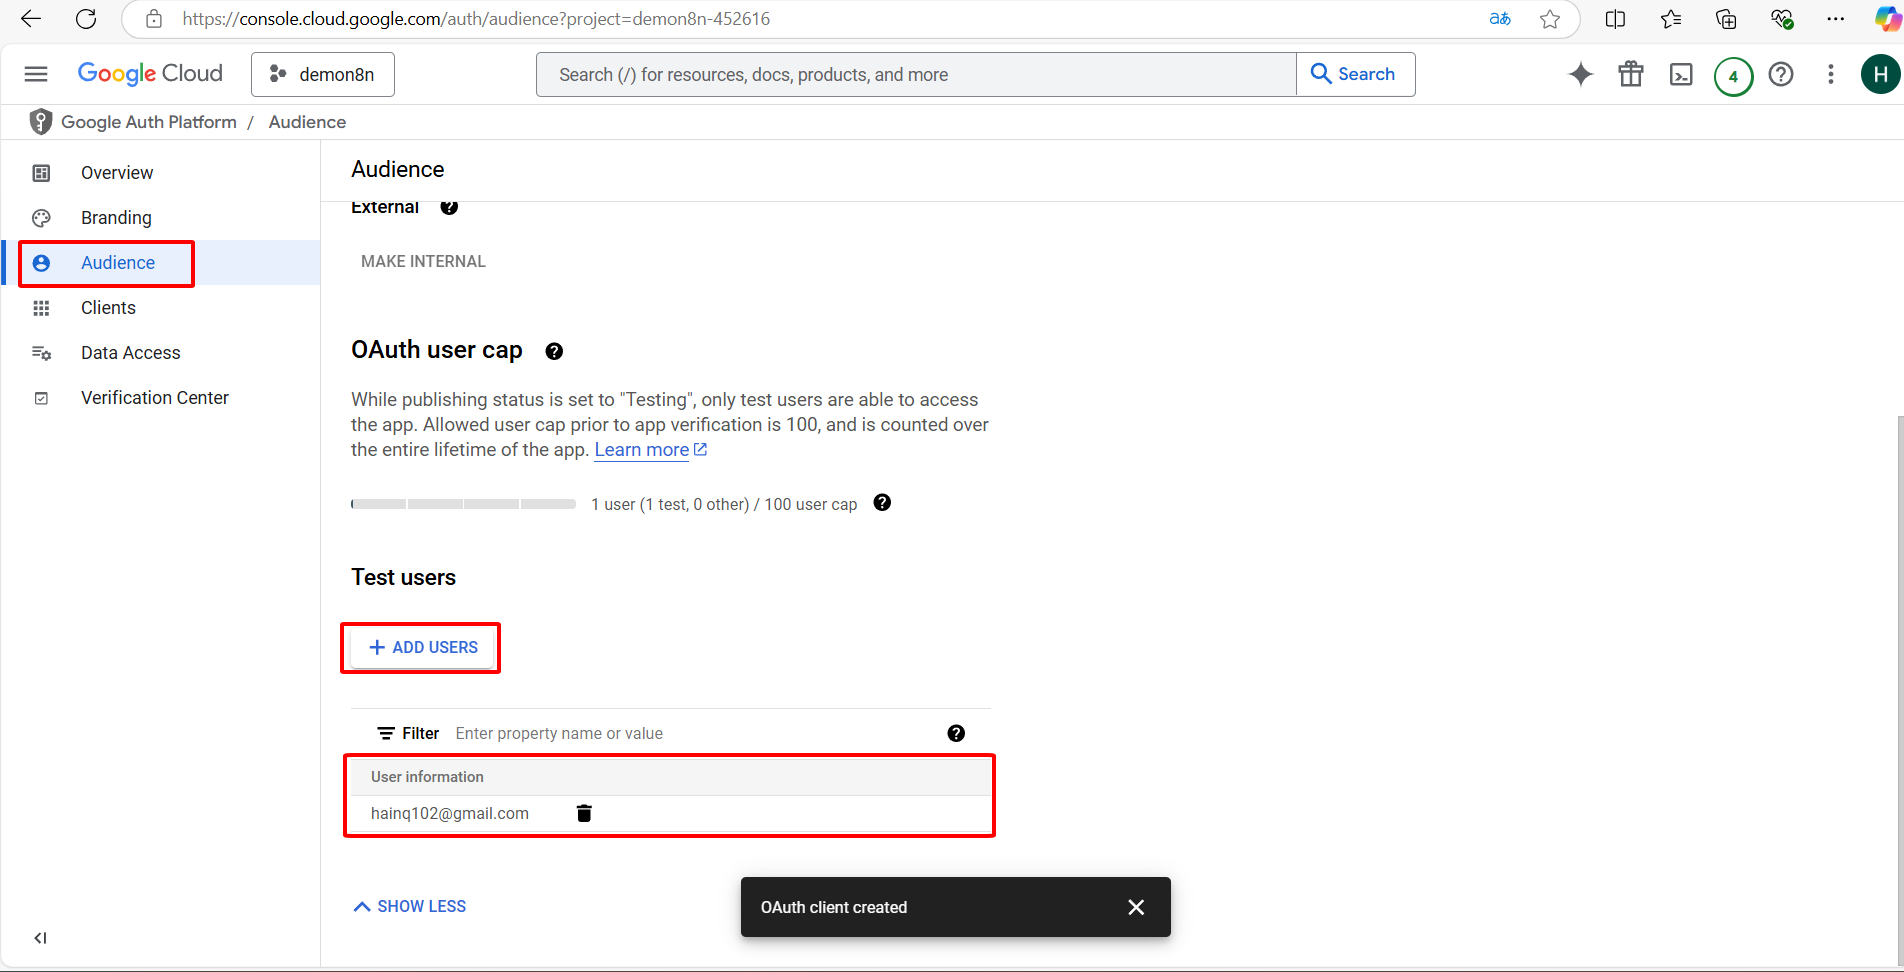
\includegraphics[width=0.95\textwidth]{images/GGcloud-15.png}
    \caption{Tạo API Together AI}
    
    \end{figure}

    \begin{figure}[H]
    \centering
    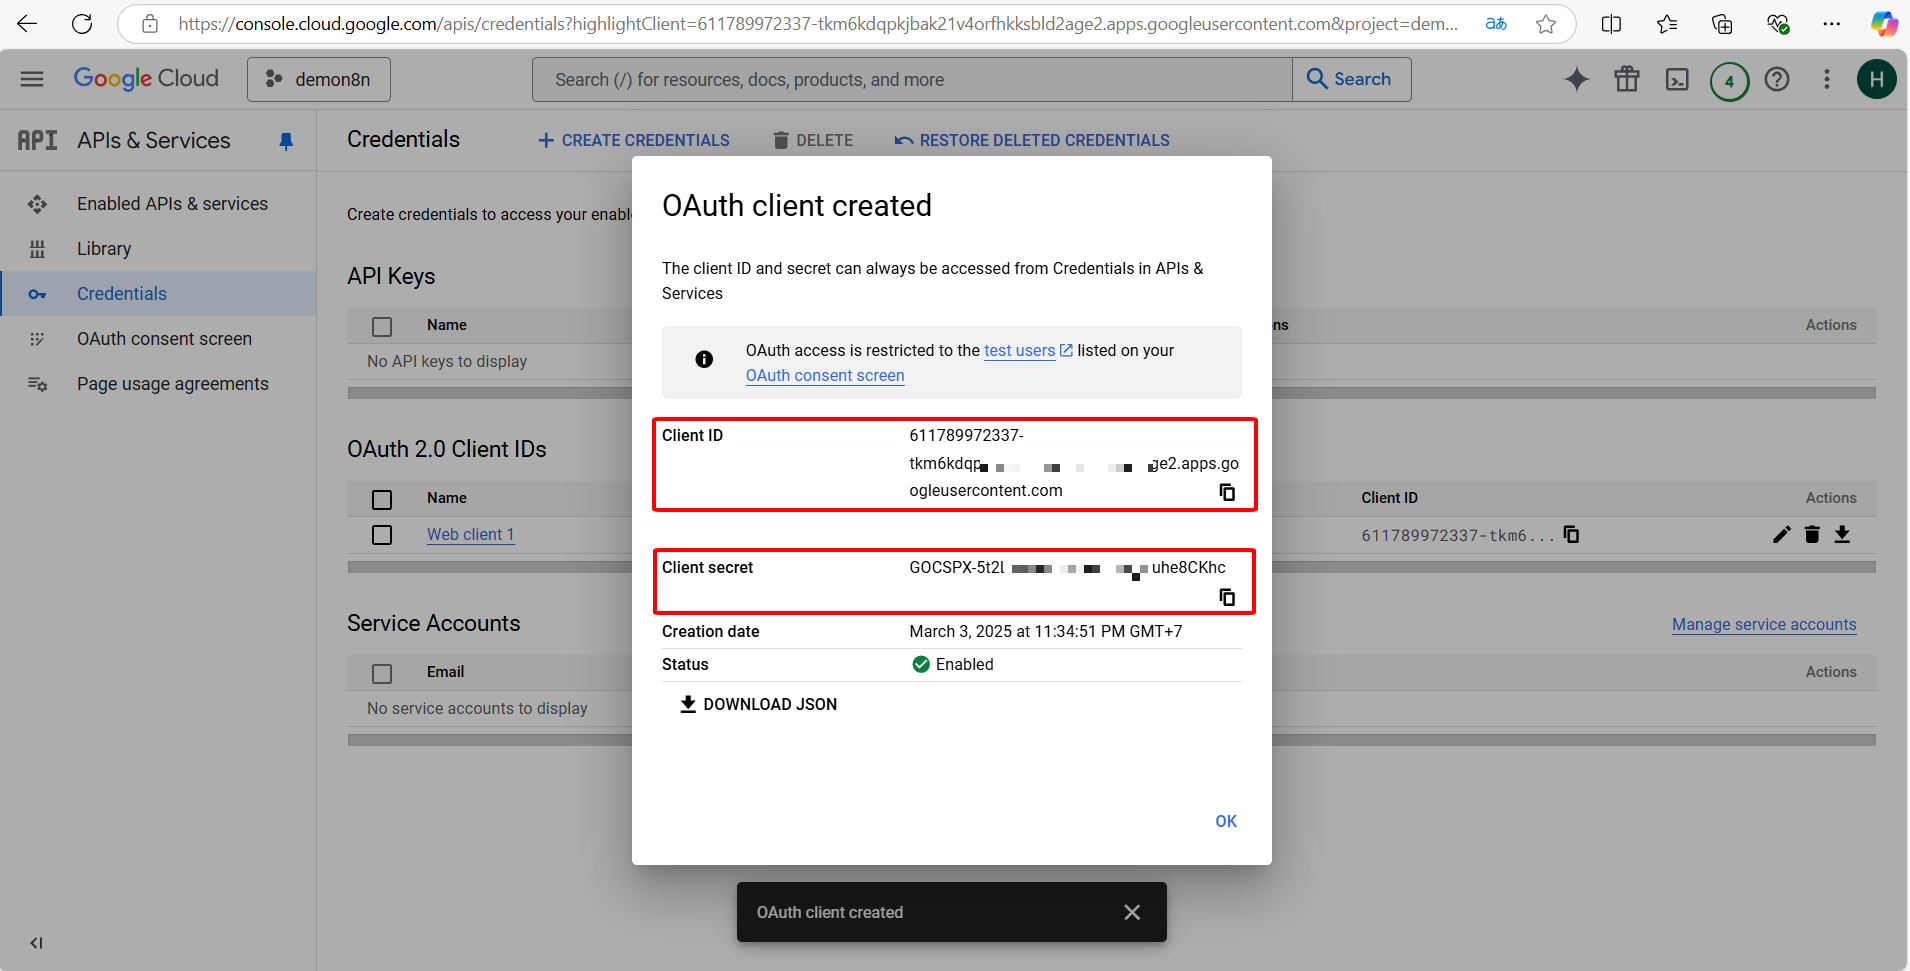
\includegraphics[width=0.95\textwidth]{images/GGcloud-13.png}
    \caption{Tạo API Together AI}
    
    \end{figure}


    
    \item \textbf{Bước 2: Tạo node "Google cloud storage" trong n8n}\\
    \begin{figure}[H]
    \centering
    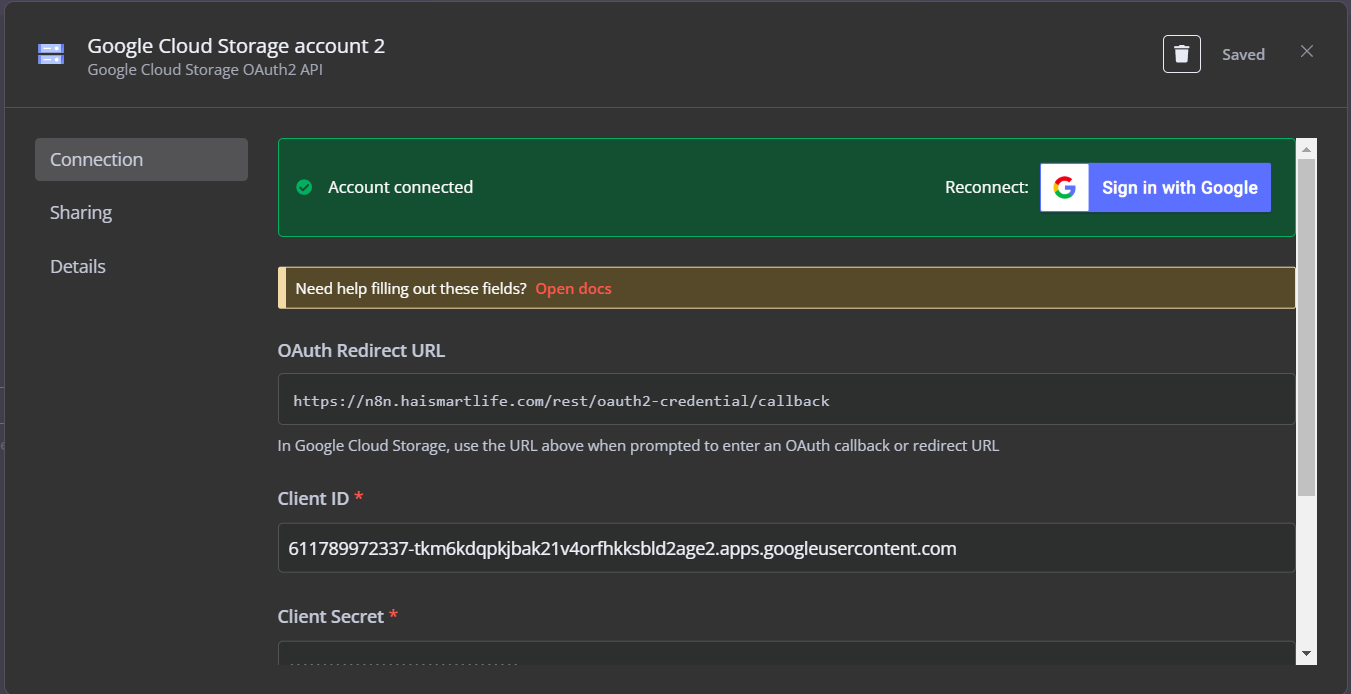
\includegraphics[width=0.95\textwidth]{images/GGcloud-16.png}
    \caption{Tạo API Elevenlabs}
    
    \end{figure}
    
 Tạo Node HTTP trong n8n, trong phần Header Auth chúng ta tạo credential như hình trên:\\
 Name: authorization\\
 Value: API vừa copy ở web Together AI\\
     \begin{figure}[H]
    \centering
    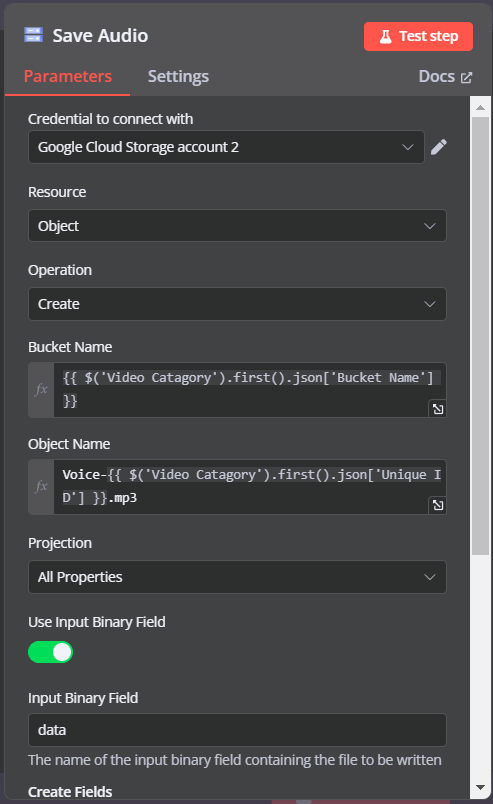
\includegraphics[width=0.6\textwidth]{images/GGcloud-17.png}
    \caption{Tạo API Elevenlabs}
    
    \end{figure}
       \verb|{{ $('Video Catagory').first().json['Bucket Name'] }}|\\
    \verb|Voice-{{ $('Video Catagory').first().json['Unique ID'] }}.mp3|

\end{itemize}

%---------------------------------
\subsection{Hailuo AI - Tạo video bằng Hailuo AI.}
\begin{itemize}[label=]
    \item \textbf{Bước 1: Tạo API key Hailuo AI} 
    
    Truy cập vào link \url{https://hailuoai.video/} \\ 
    Tìm đến API keys và copy nó ta sẽ được dãy ký tự.\\
    Lưu ý: Thêm thông tin thẻ thanh toán và sử dụng như thường, và có thể thay node này bằng node khác có chức năng tương đương thể thử.\\
    
    \begin{figure}[H]
    \centering
    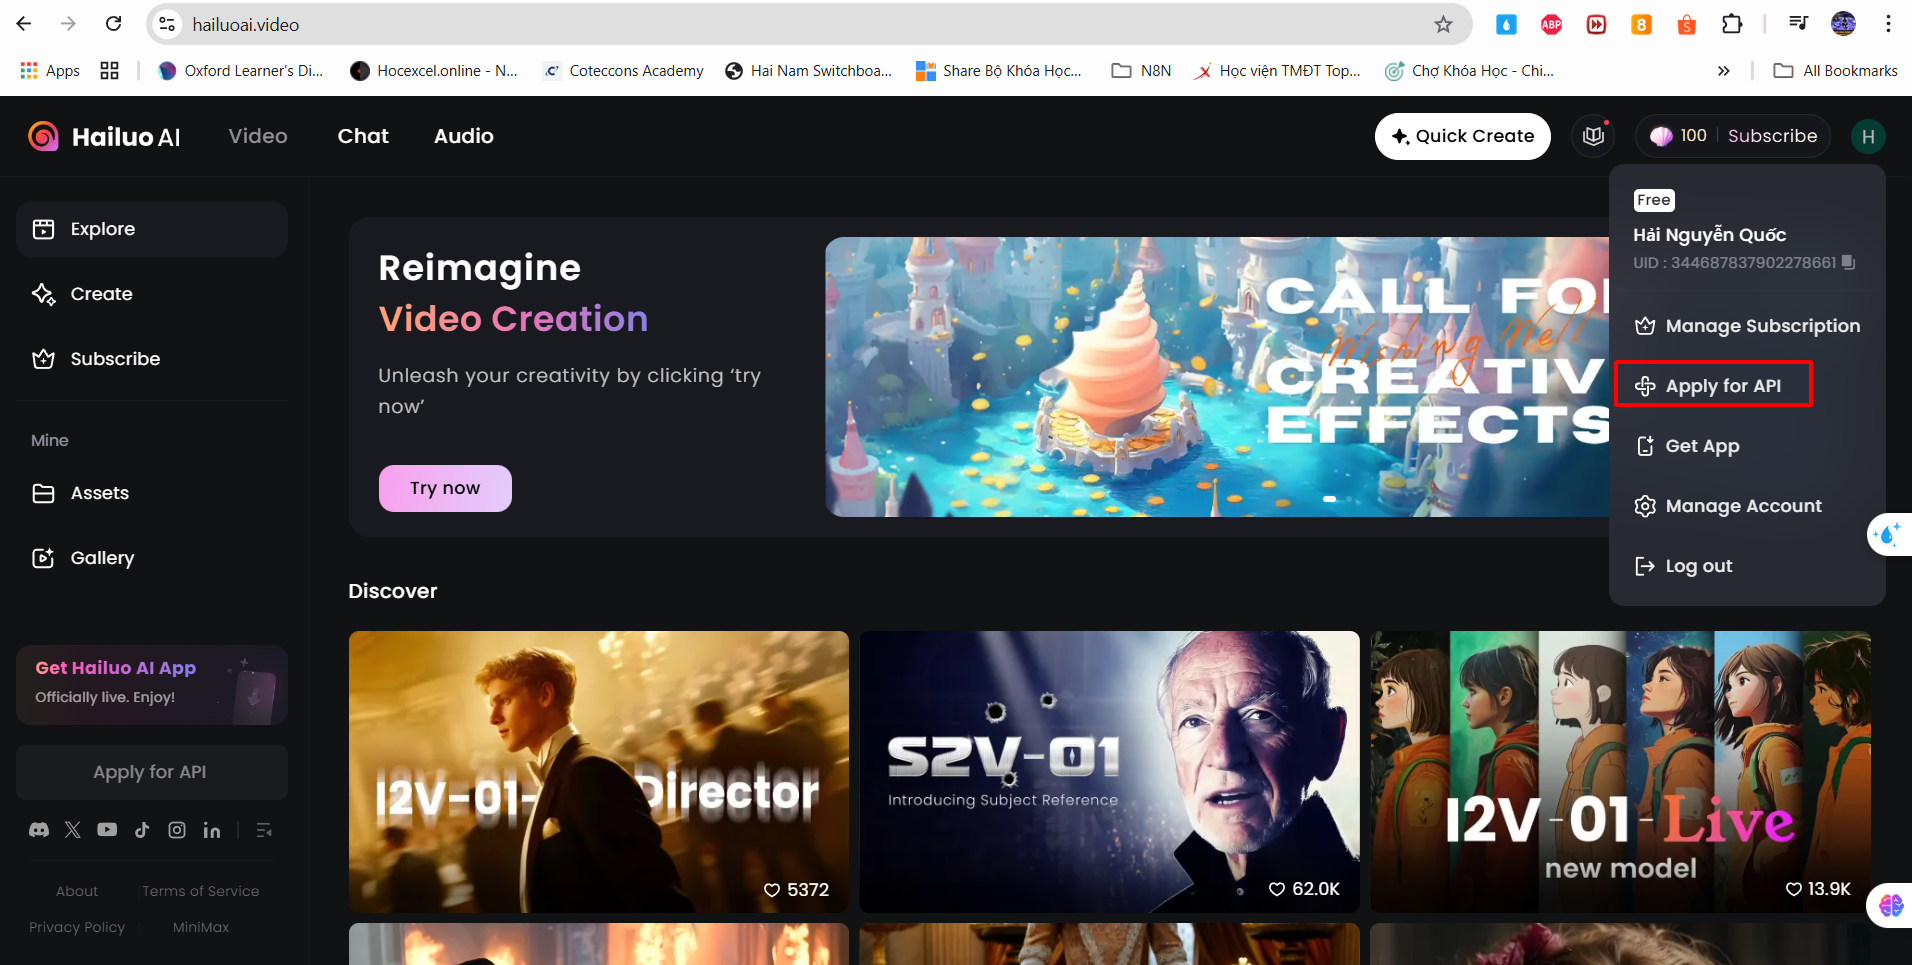
\includegraphics[width=0.95\textwidth]{images/HailuoAI.png}
    \caption{Tạo API Together AI}
    
    \end{figure}
    \item \textbf{Bước 2: Tạo node "HTTP truy cập Together AI" trong n8n}\\
    \begin{figure}[H]
    \centering
    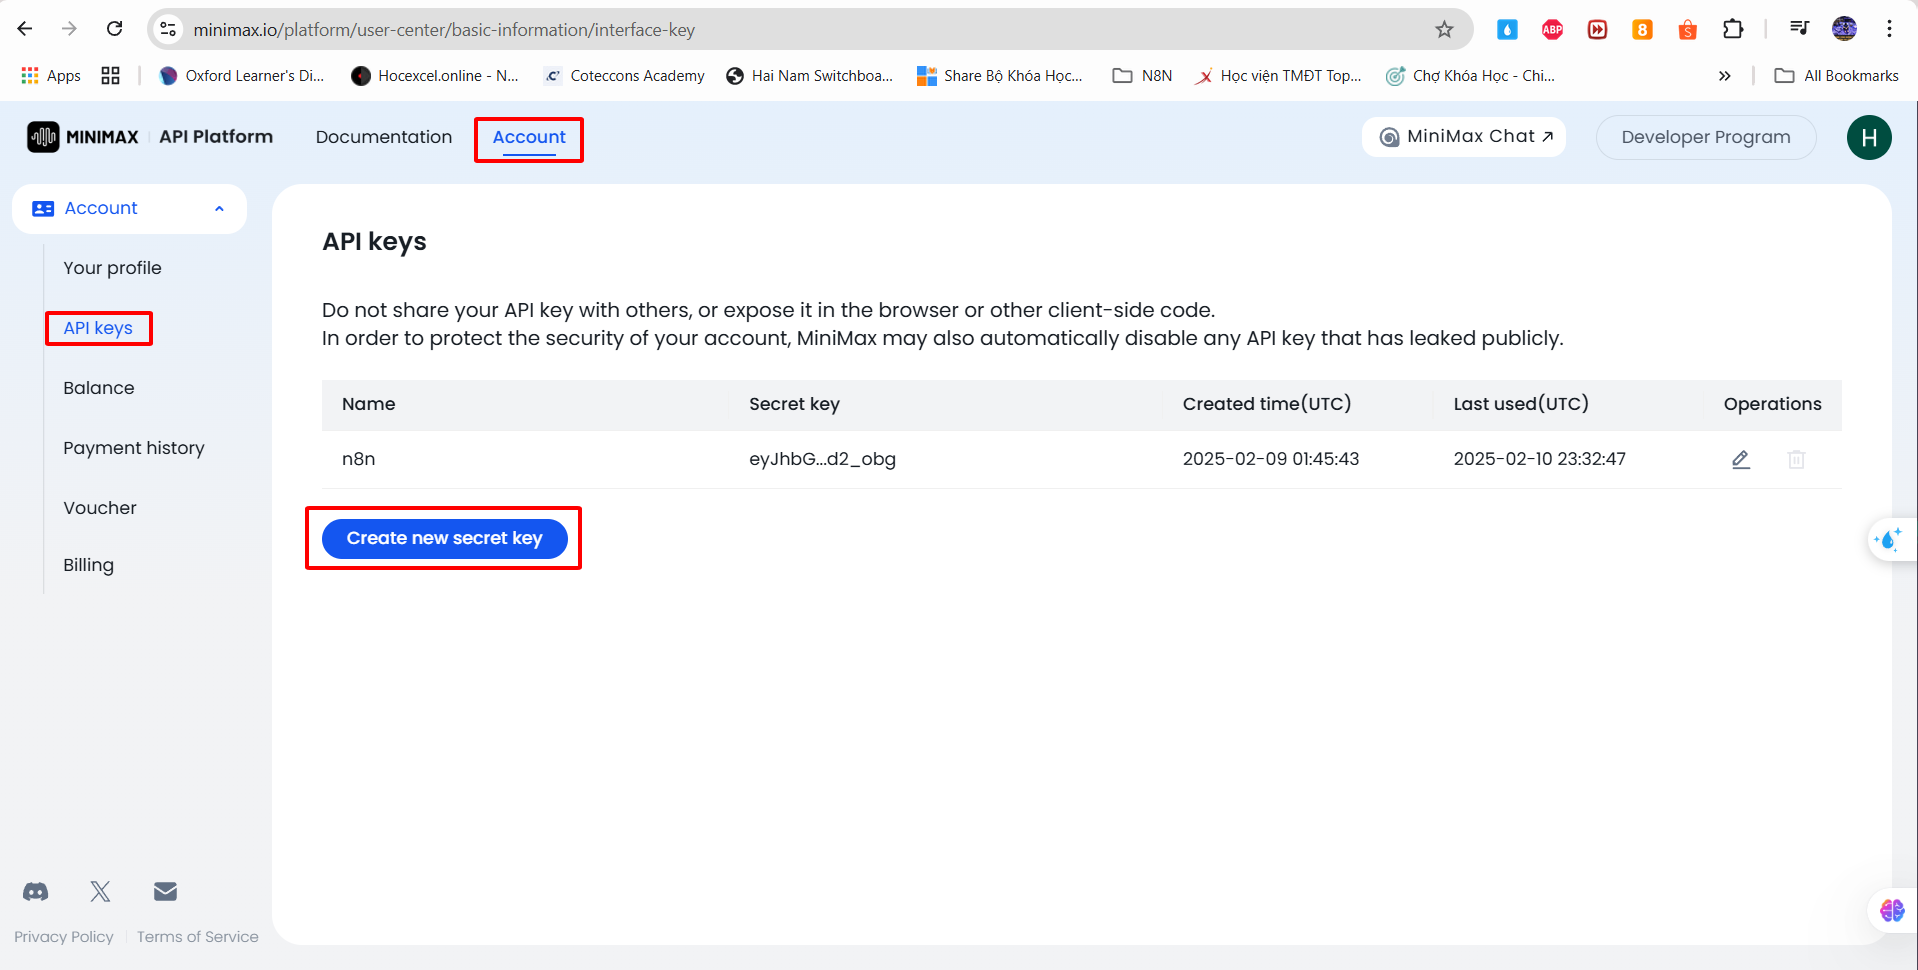
\includegraphics[width=0.95\textwidth]{images/HailuoAI-1.png}
    \caption{Tạo API Elevenlabs}
    
    \end{figure}
    \begin{figure}[H]
    \centering
    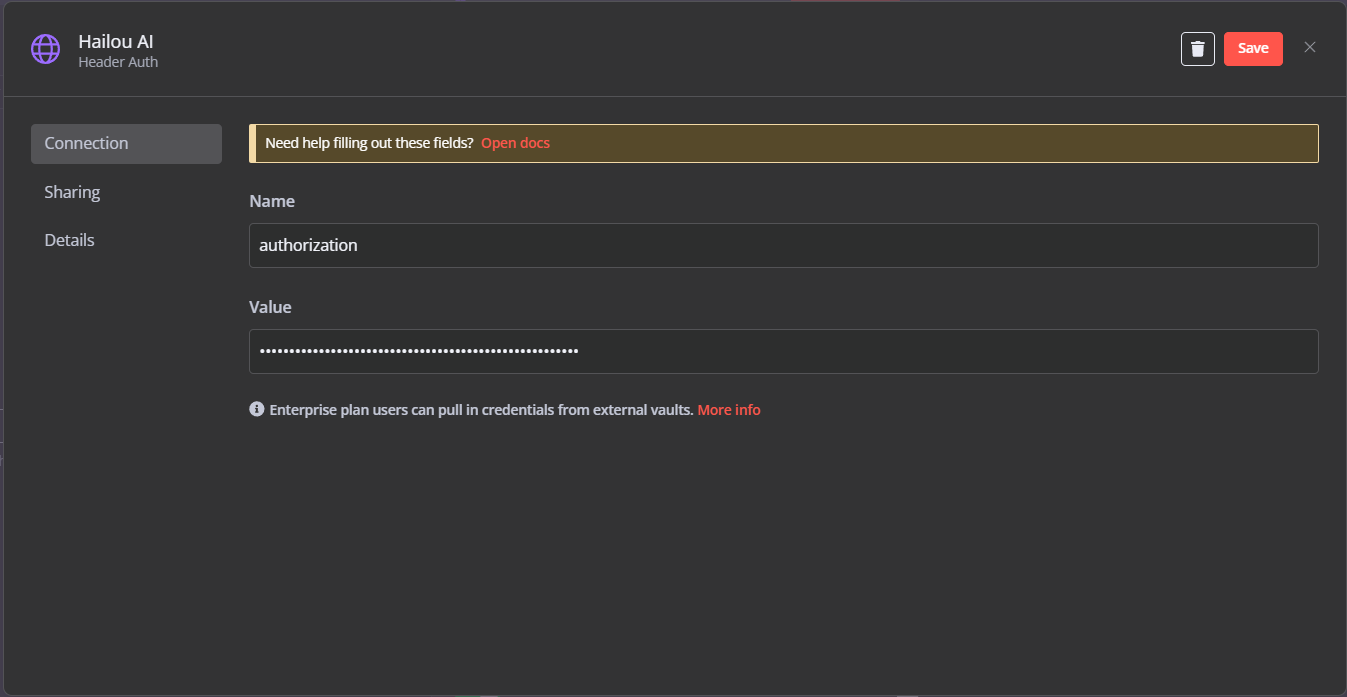
\includegraphics[width=0.95\textwidth]{images/HailuoAI-2.png}
    \caption{Tạo API Elevenlabs}
    
    \end{figure}
    
 Tạo Node HTTP trong n8n, trong phần Header Auth chúng ta tạo credential như hình trên:\\
 Name: authorization\\
 Value: Bearer API vừa copy ở web Together AI\\
 

Tại mục URL nhập: \\
"https://api.together.xyz/v1/chat/completions"\\

Tại mục Json nhập: 


Dưới đây là đoạn JSON:\\

Nơi lấy code \url{https://haismartlife.com/}


\end{itemize}


%---------------------------------
\subsection{Andynocode - Combine video.}
\begin{itemize}[label=]
    \item \textbf{Bước 1: Tạo API key Hailuo AI} 
    
    Truy cập vào link \url{https://hailuoai.video/} \\ 
    Tìm đến API keys và copy nó ta sẽ được dãy ký tự.\\
    Lưu ý: Thêm thông tin thẻ thanh toán và sử dụng như thường, và có thể thay node này bằng node khác có chức năng tương đương thể thử.\\
    
    \begin{figure}[H]
    \centering
    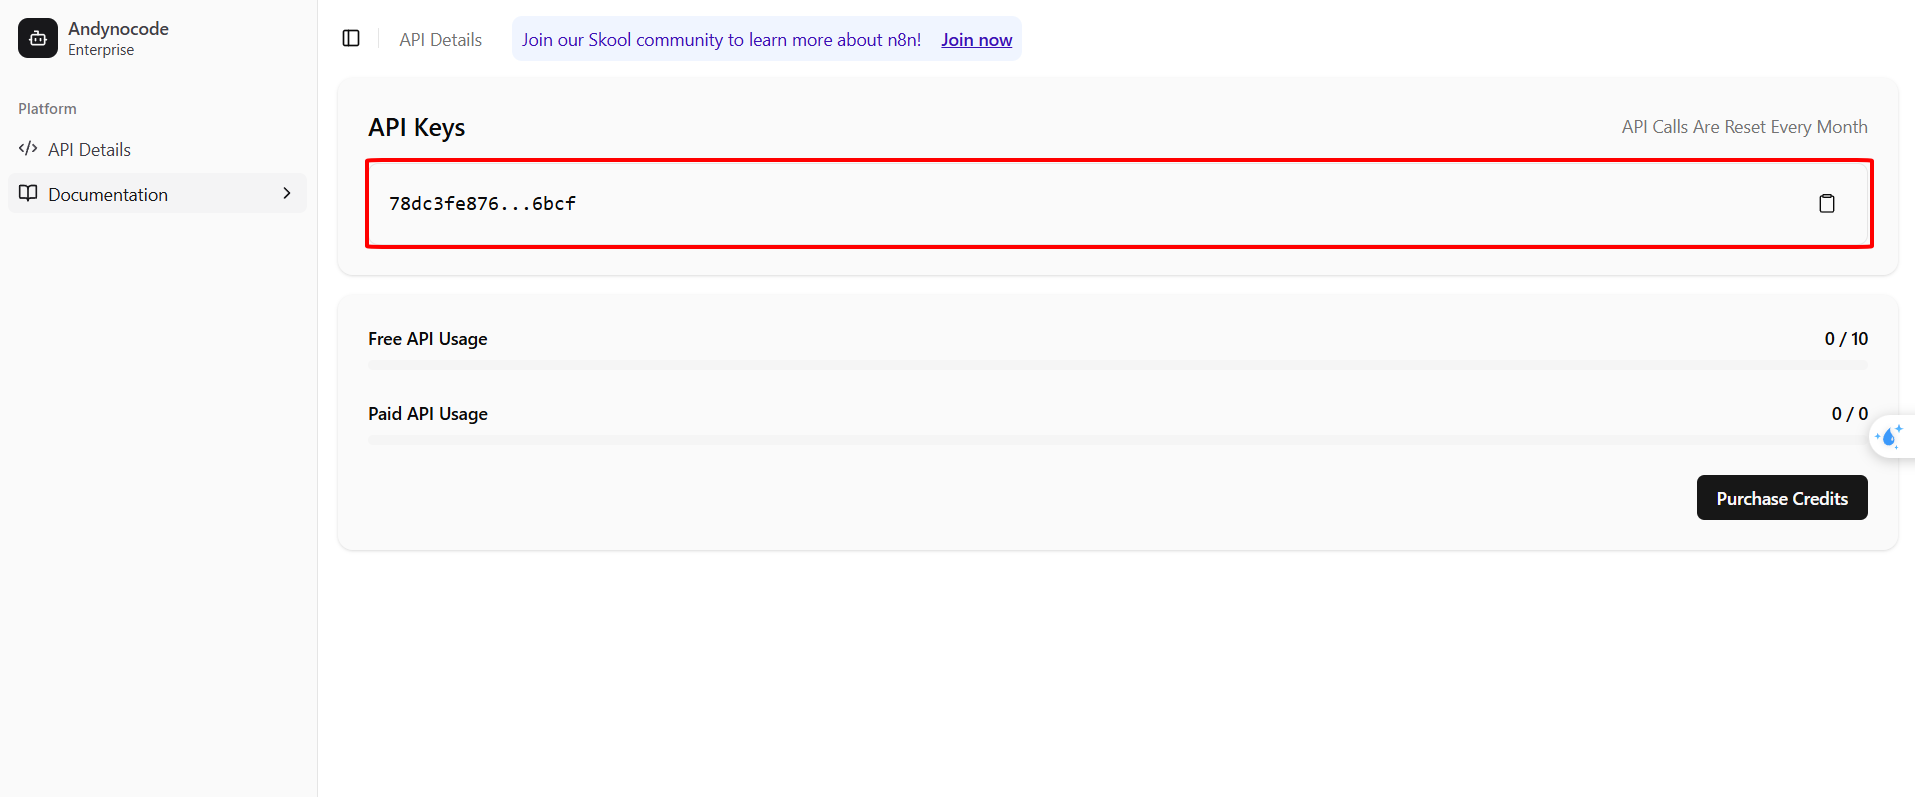
\includegraphics[width=0.95\textwidth]{images/Andy02.png}
    \caption{Tạo API Together AI}
    
    \end{figure}
    \item \textbf{Bước 2: Tạo node "HTTP truy cập Together AI" trong n8n}\\
    \begin{figure}[H]
    \centering
    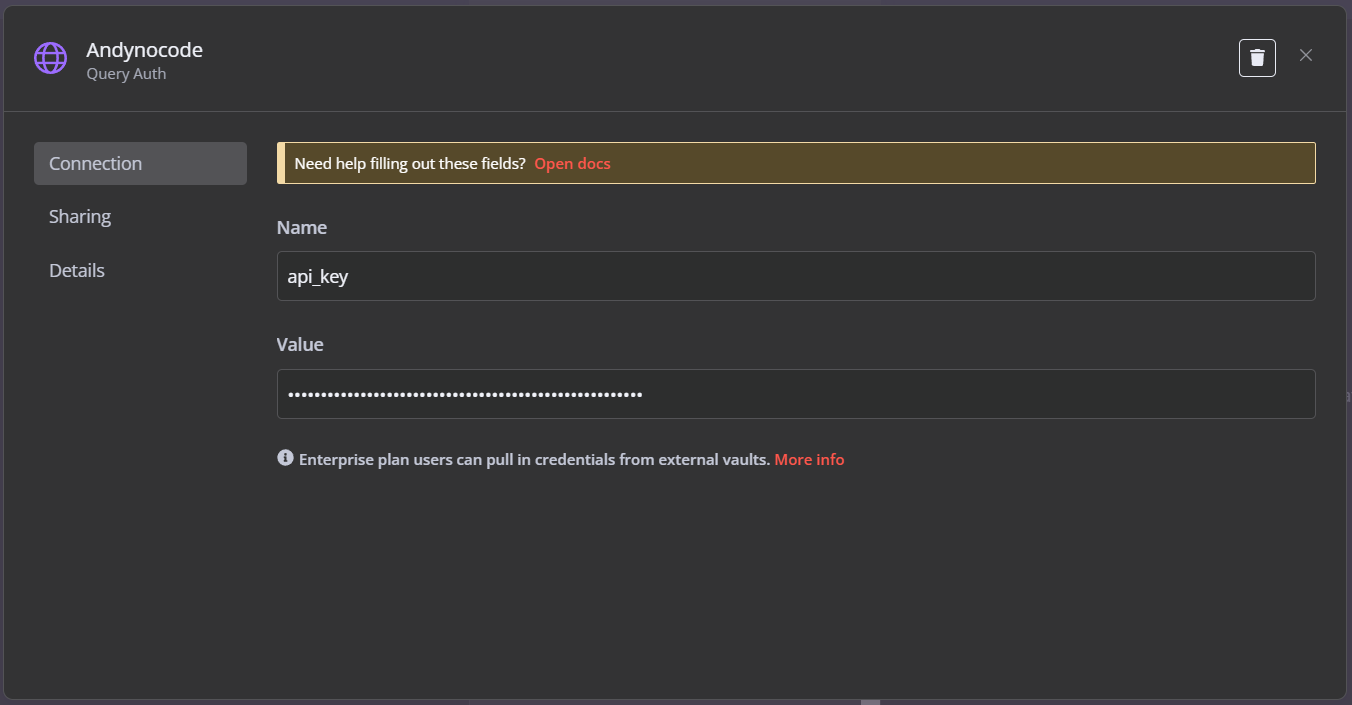
\includegraphics[width=0.95\textwidth]{images/Andy01.png}
    \caption{Tạo API Elevenlabs}
    
    \end{figure}

    
 Tạo Node HTTP trong n8n, trong phần Header Auth chúng ta tạo credential như hình trên:\\
 Name: authorization\\
 Value: Bearer API vừa copy ở web Together AI\\
 

Tại mục URL nhập: \\
"https://api.together.xyz/v1/chat/completions"\\

Tại mục Json nhập: 


Dưới đây là đoạn JSON:\\

Nơi lấy code \url{https://haismartlife.com/}


\end{itemize}

%-------------------------------------------------------------
\section{\textbf{Dự án 2: Scrape google maps lấy dữ liệu khách hàng theo lĩnh vực yêu cầu }}

\href{https://drive.google.com/drive/folders/1IktM6xKkNLkmaOFLUl4w3Ezc7U0SJUlL?usp=sharing}{\textbf{\underline {Link tải workflow}}}

    \begin{figure}[H]
    \centering
    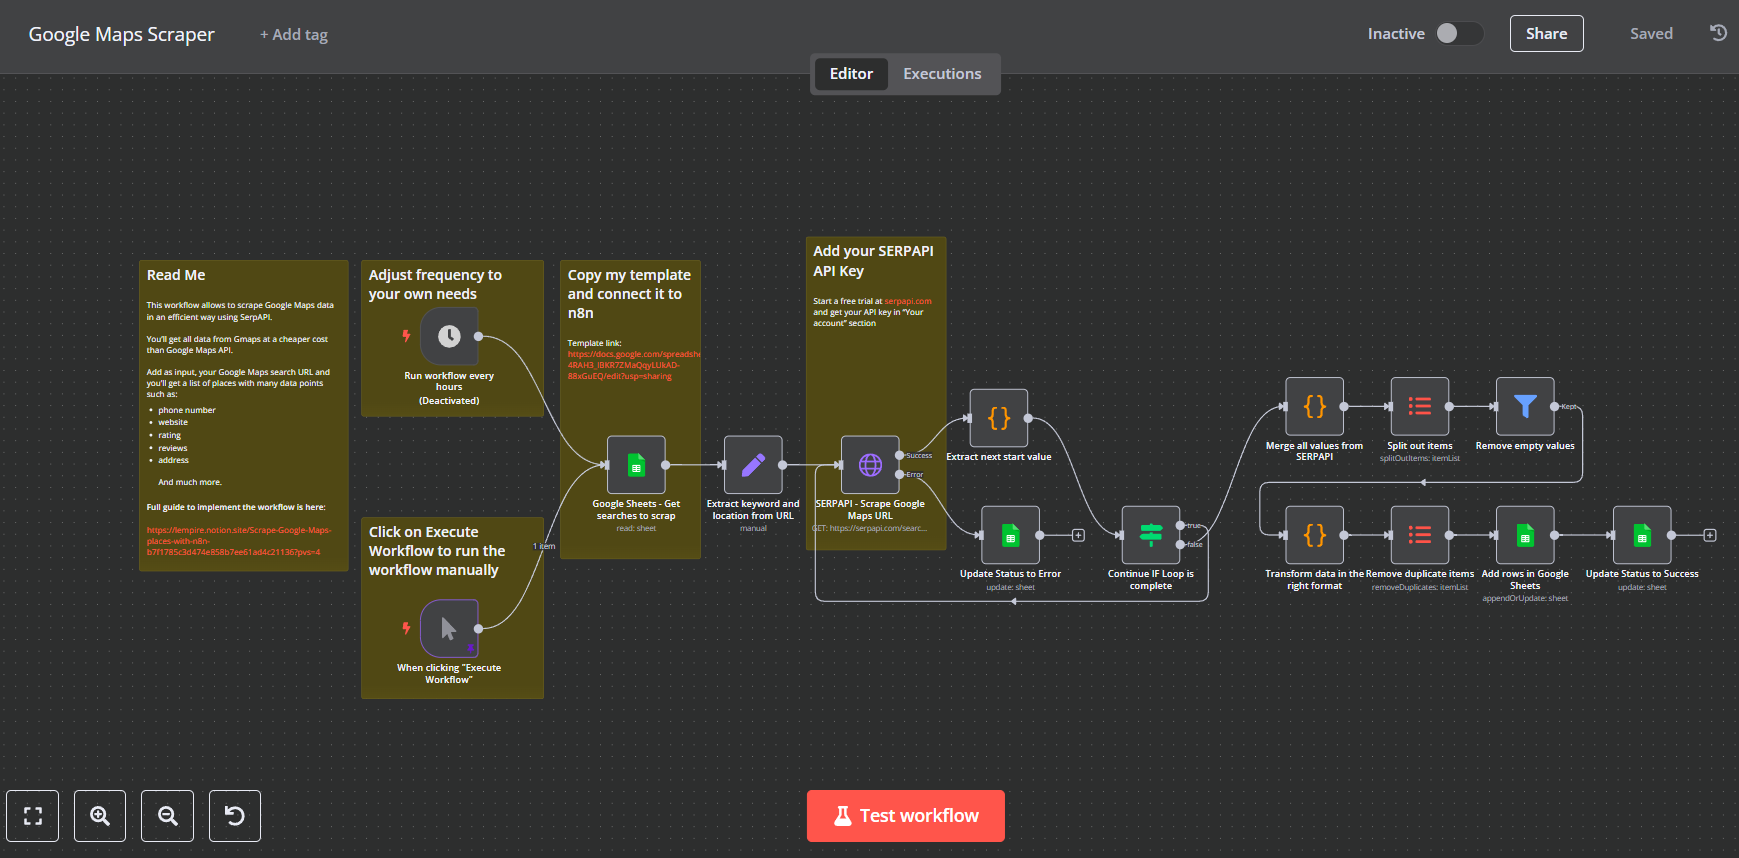
\includegraphics[width=1\textwidth]{images/2scrape01.png}
    \caption{Workflow Scrape google maps}
    \end{figure}

Đây là một workflow được thiết kế để tự động thu thập (scrape) dữ liệu từ Google Maps sử dụng SerpAPI. Workflow này được tạo trong n8n - một nền tảng tự động hóa quy trình làm việc (workflow automation platform).

\subsection{Tổng quan về Workflow}

Workflow này giúp bạn:
\begin{itemize}
  \item Thu thập thông tin về các địa điểm trên Google Maps (tên, số điện thoại, website, đánh giá, địa chỉ, v.v.)
  \item Lưu trữ dữ liệu vào Google Sheets
  \item Tự động lặp qua nhiều trang kết quả
  \item Theo dõi trạng thái của các yêu cầu scraping
\end{itemize}

\subsection{Các thành phần chính}

\begin{enumerate}
  \item \textbf{Trigger (Kích hoạt)}: Khởi chạy workflow bằng tay hoặc tự động theo lịch
  \item \textbf{API SerpAPI}: Sử dụng để truy vấn dữ liệu từ Google Maps
  \item \textbf{Google Sheets}: Lấy danh sách URL cần scrape và lưu kết quả
  \item \textbf{Code nodes}: Xử lý dữ liệu và quản lý việc phân trang
\end{enumerate}

\subsection{Hướng dẫn chi tiết từng bước}

\subsubsection{Bước 1: Chuẩn bị}

\begin{enumerate}
  \item \textbf{Tạo tài khoản SerpAPI}:
  \begin{itemize}
    \item Đăng ký tại \url{https://serpapi.com/}
    \item Lấy API key từ phần ``Your account''
  \end{itemize}

  \item \textbf{Chuẩn bị Google Sheets}:
  \begin{itemize}
    \item Sao chép template từ link: \url{https://docs.google.com/spreadsheets/d/170osqaLBql9M-4RAH3_lBKR7ZMaQqyLUkAD-88xGuEQ/edit?usp=sharing}
    \item Sheet này có 2 tab chính:
    \begin{itemize}
      \item \textbf{Scrape Maps}: Nơi bạn thêm URL Google Maps cần scrape
      \item \textbf{Result}: Nơi lưu kết quả thu được
    \end{itemize}
  \end{itemize}
\end{enumerate}

\subsubsection{Bước 2: Thiết lập workflow trong n8n}

\begin{enumerate}
  \item \textbf{Tạo workflow mới} trong n8n

  \item \textbf{Thêm Trigger node}:
  \begin{itemize}
    \item Có 2 lựa chọn:
    \begin{itemize}
      \item ``When clicking Execute Workflow'' (chạy thủ công)
      \item ``Run workflow every hours'' (chạy tự động theo lịch)
    \end{itemize}
  \end{itemize}

  \item \textbf{Kết nối với Google Sheets}:
  \begin{itemize}
    \item Thêm node ``Google Sheets - Get searches to scrap''
    \item Kết nối với Google account của bạn
    \item Chọn document ID của sheet đã sao chép
    \item Chọn sheet tab ``Scrape Maps''
  \end{itemize}

  \item \textbf{Xử lý URL từ Google Maps}:
  \begin{itemize}
    \item Thêm node ``Extract keyword and location from URL''
    \item Node này sử dụng regular expression để trích xuất:
    \begin{itemize}
      \item Từ khóa tìm kiếm (\texttt{keyword})
      \item Tọa độ địa lý (\texttt{geo})
    \end{itemize}
  \end{itemize}

  \item \textbf{Kết nối với SerpAPI}:
  \begin{itemize}
    \item Thêm node ``SERPAPI - Scrape Google Maps URL''
    \item Cấu hình các tham số:
    \begin{itemize}
      \item \texttt{engine}: google\_maps
      \item \texttt{q}: Từ khóa đã trích xuất
      \item \texttt{ll}: Tọa độ địa lý đã trích xuất
      \item \texttt{type}: search
      \item \texttt{start}: Tham số phân trang (bắt đầu từ 0)
    \end{itemize}
    \item Thêm API key SerpAPI vào phần credentials
  \end{itemize}

  \item \textbf{Xử lý phân trang}:
  \begin{itemize}
    \item Thêm node ``Extract next start value''
    \item Node này kiểm tra nếu có trang tiếp theo và trích xuất tham số \texttt{start} để tiếp tục quá trình scraping
  \end{itemize}

  \item \textbf{Điều kiện lặp}:
  \begin{itemize}
    \item Thêm node ``Continue IF Loop is complete''
    \item Kiểm tra 2 điều kiện:
    \begin{itemize}
      \item \texttt{\$json.search\_parameters.start} <= 40 (giới hạn số trang)
      \item \texttt{\$json.serpapi\_pagination.next} không rỗng (còn trang tiếp theo)
    \end{itemize}
    \item Nếu đúng → quay lại node SERPAPI để lấy trang tiếp theo
    \item Nếu sai → tiến hành xử lý dữ liệu đã thu thập
  \end{itemize}

  \item \textbf{Xử lý dữ liệu}:
  \begin{itemize}
    \item Thêm node ``Merge all values from SERPAPI'' để gộp kết quả từ tất cả các trang
    \item Thêm node ``Split out items'' để tách từng mục riêng lẻ
    \item Thêm node ``Remove empty values'' để loại bỏ giá trị rỗng
    \item Thêm node ``Transform data in the right format'' để định dạng dữ liệu
    \item Thêm node ``Remove duplicate items'' để loại bỏ các mục trùng lặp
  \end{itemize}

  \item \textbf{Lưu kết quả vào Google Sheets}:
  \begin{itemize}
    \item Thêm node ``Add rows in Google Sheets''
    \item Kết nối với Google account
    \item Chọn document ID và sheet tab ``Result''
    \item Ánh xạ các trường dữ liệu vào các cột tương ứng
  \end{itemize}

  \item \textbf{Cập nhật trạng thái}:
  \begin{itemize}
    \item Thêm node ``Update Status to Success'' để cập nhật trạng thái thành công (tick xanh)
    \item Thêm node ``Update Status to Error'' để cập nhật trạng thái lỗi (X đỏ)
  \end{itemize}
\end{enumerate}

\subsubsection{Bước 3: Chạy và quản lý workflow}

\begin{enumerate}
  \item \textbf{Cách thêm URL Google Maps cần scrape}:
  \begin{itemize}
    \item Mở Google Sheet đã tạo
    \item Vào tab ``Scrape Maps''
    \item Thêm URL Google Maps vào cột URL, Vào GG maps nhập từ khoá về ngành bạn muốn quét, sau đó copy link 
  \end{itemize}

  \item \textbf{Chạy workflow}:
  \begin{itemize}
    \item Chọn node ``When clicking Execute Workflow'' và nhấn ``Execute Workflow''
    \item Hoặc bật node ``Run workflow every hours'' để chạy tự động
  \end{itemize}

  \item \textbf{Kiểm tra kết quả}:
  \begin{itemize}
    \item Kết quả sẽ được lưu vào tab ``Result'' của Google Sheet
    \item Trạng thái của mỗi URL sẽ được cập nhật trong tab ``Scrape Maps'':
    \begin{itemize}
      \item tick xanh: Thành công
      \item X đỏ: Lỗi
    \end{itemize}
  \end{itemize}
\end{enumerate}

\subsection{Chi tiết về xử lý dữ liệu}

\subsubsection{Node ``Extract keyword and location from URL''}
\begin{verbatim}
// Trích xuất từ khóa từ URL
{{ $json.URL.match(/\/search\/(.*?)\//)[1] }}

// Trích xuất tọa độ địa lý từ URL
{{ $json.URL.match(/(@[^\/?]+)/)[1] }}
\end{verbatim}

\subsubsection{Node ``Extract next start value''}
\begin{verbatim}
let nextUrl

if ($json && $json["serpapi_pagination"] && $json["serpapi_pagination"]["next"]) {
    nextUrl = $json["serpapi_pagination"]["next"];
    
    $input.item.json.start = nextUrl.split('&').find(param => 
        param.startsWith('start=')).split('=')[1];
}

return $input.item;
\end{verbatim}

\subsubsection{Node ``Merge all values from SERPAPI''}
\begin{verbatim}
const allData = []

let counter = 0;
do {
  try {
    const items = $items("SERPAPI - Scrape Google Maps URL", 0, counter)
                  .map(item => item.json.local_results);
    allData.push.apply(allData, items);
  } catch (error) {
    return [{json: {allData}}];  
  }

  counter++;
} while(true);
\end{verbatim}

\subsection{Dữ liệu được thu thập}

Workflow này thu thập nhiều thông tin từ mỗi địa điểm trên Google Maps, bao gồm:

\begin{itemize}
  \item \textbf{place\_id}: ID định danh duy nhất của địa điểm
  \item \textbf{title}: Tên địa điểm
  \item \textbf{phone}: Số điện thoại
  \item \textbf{website}: Trang web
  \item \textbf{rating}: Điểm đánh giá
  \item \textbf{reviews}: Số lượng đánh giá
  \item \textbf{type}: Loại địa điểm
  \item \textbf{address}: Địa chỉ
  \item \textbf{hours}: Giờ làm việc
  \item \textbf{operating\_hours}: Chi tiết giờ hoạt động
  \item \textbf{service\_options}: Các tùy chọn dịch vụ
  \item \textbf{thumbnail}: Hình thu nhỏ
  \item và nhiều thông tin khác
\end{itemize}

\subsection{Ưu điểm của workflow này}

\begin{enumerate}
  \item \textbf{Hiệu quả về chi phí}: Sử dụng SerpAPI thay vì Google Maps API chính thức (thường đắt hơn)
  \item \textbf{Tự động hóa}: Có thể chạy tự động theo lịch
  \item \textbf{Quản lý tốt}: Theo dõi trạng thái scraping của từng URL
  \item \textbf{Toàn diện}: Thu thập nhiều loại thông tin hữu ích
  \item \textbf{Chống trùng lặp}: Loại bỏ các dữ liệu trùng lặp
\end{enumerate}

\subsection{Các lưu ý quan trọng}

\begin{enumerate}
  \item \textbf{Giới hạn API}: SerpAPI có giới hạn số lượng requests trong gói miễn phí, nên theo dõi việc sử dụng
  \item \textbf{Giới hạn phân trang}: Workflow được cấu hình để dừng sau 40 kết quả (điều này có thể điều chỉnh)
  \item \textbf{Quyền Google Sheets}: Đảm bảo tài khoản Google có quyền truy cập đầy đủ vào Google Sheet
  \item \textbf{Kiểm tra định kỳ}: Kiểm tra tab ``Scrape Maps'' để xem trạng thái của các yêu cầu scraping
\end{enumerate}

\subsection{Cách điều chỉnh workflow}

\begin{enumerate}
  \item \textbf{Thay đổi giới hạn phân trang}:
  \begin{itemize}
    \item Chỉnh sửa điều kiện trong node ``Continue IF Loop is complete''
    \item Thay đổi giá trị \texttt{40} thành số trang mong muốn
  \end{itemize}

  \item \textbf{Thay đổi tần suất tự động chạy}:
  \begin{itemize}
    \item Chỉnh sửa node ``Run workflow every hours''
    \item Thay đổi tần suất từ ``hours'' thành ``days'', ``minutes'', v.v.
  \end{itemize}

  \item \textbf{Thêm trường dữ liệu}:
  \begin{itemize}
    \item Chỉnh sửa ánh xạ trong node ``Add rows in Google Sheets''
    \item Thêm cột mới vào Google Sheet
  \end{itemize}
\end{enumerate}

Với việc thiết lập đúng cách, workflow này sẽ giúp bạn thu thập dữ liệu từ Google Maps một cách hiệu quả và tự động, phù hợp cho nhiều mục đích như nghiên cứu thị trường, tìm kiếm khách hàng tiềm năng, hoặc phân tích cạnh tranh.

\clearpage
%---------------------------------------------------------------------
\section{\textbf{Dự án 3: Tạo chatbot theo dõi thu chi bằng n8n qua Telegram }}

\href{https://drive.google.com/drive/folders/1tumFktBej5fgHsKSuYDtnL2V0W5OI9nk?usp=sharing}{\textbf{\underline {Link tải workflow}}}

\begin{figure}[h]
    \centering
    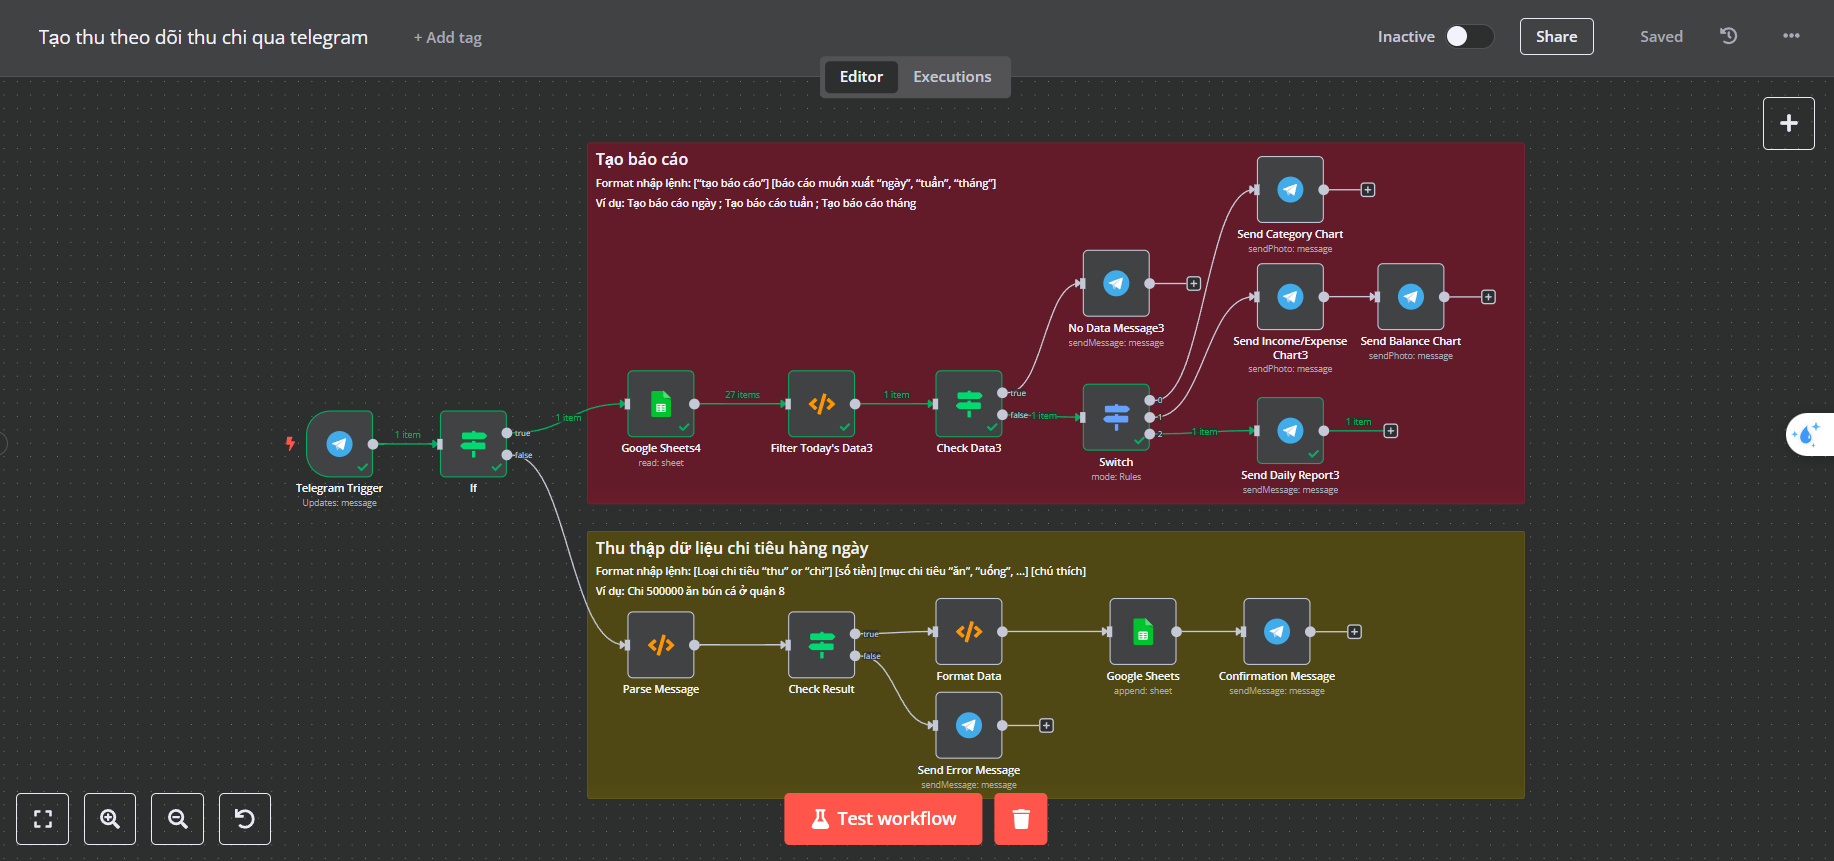
\includegraphics[width=1\textwidth]{images/3thuchi01.png}
    \caption{Workflow theo dõi thu chi}
    
\end{figure}

Đây là một workflow phức tạp nhưng rất hữu ích được xây dựng trên nền tảng n8n để theo dõi tài chính cá nhân thông qua một bot Telegram. Bài viết sẽ phân tích chi tiết các thành phần chính, ưu điểm và cách thiết lập.

\subsection{Tổng quan về workflow}

Workflow này tạo ra một bot Telegram cho phép người dùng:
\begin{enumerate}
    \item Ghi lại các khoản thu chi hàng ngày một cách nhanh chóng
    \item Tạo báo cáo tài chính theo ngày, tuần, tháng với biểu đồ trực quan
    \item Lưu trữ dữ liệu vào Google Sheets để dễ dàng theo dõi và phân tích
\end{enumerate}

\subsection{Các thành phần chính}

\subsubsection{Thu thập dữ liệu từ người dùng}
Bot nhận tin nhắn từ người dùng theo các định dạng:
\begin{itemize}
    \item Nhập khoản chi tiêu: \texttt{[thu/chi] [số tiền] [danh mục] [ghi chú]}
    \begin{itemize}
        \item Ví dụ: \texttt{Chi 500000 ăn bún cá ở quận 8}
    \end{itemize}
    \item Yêu cầu báo cáo: \texttt{Tạo báo cáo [ngày/tuần/tháng]}
    \begin{itemize}
        \item Ví dụ: \texttt{Tạo báo cáo tuần}
    \end{itemize}
\end{itemize}

\subsubsection{Lưu trữ dữ liệu}
\begin{itemize}
    \item Sử dụng Google Sheets làm cơ sở dữ liệu
    \item Mỗi giao dịch được ghi lại với các thông tin: ngày tháng, loại (thu/chi), số tiền, danh mục, ghi chú
\end{itemize}

\subsubsection{Phân tích dữ liệu}
\begin{itemize}
    \item Node Function xử lý phức tạp để tính toán tổng thu, tổng chi và số dư
    \item Phân loại chi tiêu theo danh mục
    \item So sánh với tuần trước để thấy xu hướng
    \item Đưa ra gợi ý tiết kiệm
\end{itemize}

\subsubsection{Tạo báo cáo trực quan}
\begin{itemize}
    \item Sử dụng QuickChart.io để tạo 3 loại biểu đồ:
    \begin{itemize}
        \item Biểu đồ cột thể hiện thu/chi của 4 tuần gần nhất
        \item Biểu đồ đường thể hiện biến động số dư
        \item Biểu đồ tròn phân loại chi tiêu theo danh mục
    \end{itemize}
\end{itemize}

\subsection{Luồng hoạt động}

\begin{enumerate}
    \item \textbf{Nhận tin nhắn từ Telegram}: Node Telegram Trigger bắt tin nhắn từ người dùng
    \item \textbf{Phân loại yêu cầu}: If node kiểm tra xem người dùng muốn nhập giao dịch hay tạo báo cáo
    \item \textbf{Xử lý giao dịch mới}:
    \begin{itemize}
        \item Parse Message phân tích tin nhắn của người dùng
        \item Format Data chuẩn hóa dữ liệu
        \item Google Sheets lưu dữ liệu vào bảng tính
        \item Confirmation Message gửi xác nhận đã lưu giao dịch
    \end{itemize}
    \item \textbf{Tạo báo cáo}:
    \begin{itemize}
        \item Google Sheets4 lấy dữ liệu từ bảng tính
        \item Filter Today's Data3 xử lý và phân tích dữ liệu
        \item Check Data3 kiểm tra xem có dữ liệu không
        \item Switch phân loại loại báo cáo (ngày/tuần/tháng)
        \item Các node Send gửi báo cáo và biểu đồ trực quan
    \end{itemize}
\end{enumerate}

\subsection{Ưu điểm của workflow}

\begin{enumerate}
    \item \textbf{Đơn giản hóa việc theo dõi tài chính}: Nhập giao dịch nhanh chóng qua Telegram mà không cần mở ứng dụng phức tạp
    \item \textbf{Tự động hóa phân tích}: Tự động tính toán, phân loại và so sánh dữ liệu
    \item \textbf{Báo cáo trực quan}: Biểu đồ giúp dễ dàng nắm bắt tình hình tài chính
    \item \textbf{Dễ tiếp cận}: Sử dụng Telegram - ứng dụng nhắn tin phổ biến làm giao diện
    \item \textbf{Lưu trữ an toàn}: Dữ liệu được lưu trong Google Sheets, dễ dàng truy cập và sao lưu
    \item \textbf{Đa ngôn ngữ}: Workflow hỗ trợ tiếng Việt, dễ dàng mở rộng cho các ngôn ngữ khác
\end{enumerate}

\subsection{Hướng dẫn thiết lập cho người mới}

\subsubsection{Bước 1: Chuẩn bị tài khoản và công cụ}
\begin{itemize}
    \item Đăng ký tài khoản \href{https://n8n.io}{n8n}
    \item Tạo bot Telegram thông qua \href{https://t.me/botfather}{BotFather}
    \item Chuẩn bị một Google Sheet với các cột: date, type, amount, category, note, timestamp
\end{itemize}

\subsubsection{Bước 2: Cấu hình webhook và kết nối API}
\begin{enumerate}
    \item Cài đặt credentials cho Telegram API trong n8n
    \item Cấu hình OAuth cho Google Sheets
    \item Thiết lập webhook cho Telegram Trigger
\end{enumerate}

\subsubsection{Bước 3: Tạo cấu trúc workflow}
\begin{enumerate}
    \item Bắt đầu với Telegram Trigger
    \item Thêm If node để phân loại yêu cầu
    \item Tạo nhánh xử lý nhập giao dịch
    \item Tạo nhánh tạo báo cáo
\end{enumerate}

\subsubsection{Bước 4: Cấu hình chi tiết cho từng node}
\begin{enumerate}
    \item \textbf{Parse Message}: Copy code JavaScript từ workflow mẫu để xử lý tin nhắn
    \item \textbf{Filter Today's Data3}: Copy code để phân tích và tạo biểu đồ  
    \item \textbf{Google Sheets}: Cấu hình kết nối với bảng tính của bạn
    \item \textbf{Send nodes}: Điều chỉnh định dạng tin nhắn và caption cho phù hợp
\end{enumerate}

\subsubsection{Bước 5: Kiểm tra và tối ưu}
\begin{enumerate}
    \item Chạy thử workflow với các loại tin nhắn khác nhau
    \item Kiểm tra xem dữ liệu có được lưu chính xác không
    \item Điều chỉnh các định dạng báo cáo và biểu đồ theo nhu cầu
\end{enumerate}

\subsection{Khả năng mở rộng}

Workflow này có thể được mở rộng với các tính năng:
\begin{enumerate}
    \item Thêm báo cáo theo quý/năm
    \item Tạo hệ thống ngân sách và cảnh báo khi vượt quá ngân sách
    \item Thêm chức năng xuất báo cáo dưới dạng PDF
    \item Thêm nhắc nhở thanh toán định kỳ
    \item Tích hợp với các API tài chính để tự động cập nhật giao dịch
\end{enumerate}

\subsection{Kết luận}

Với workflow này, việc theo dõi tài chính cá nhân trở nên đơn giản và trực quan hơn, giúp người dùng dễ dàng nắm bắt tình hình tài chính và đưa ra các quyết định tài chính thông minh hơn. Đây là một ví dụ điển hình về cách n8n có thể được sử dụng để tự động hóa và tối ưu các tác vụ trong cuộc sống hàng ngày mà không cần đến kỹ năng lập trình phức tạp.

\clearpage
%----------------------------------------------------------------
\section{\textbf{Dự án 4: Tạo trợ lý ảo bằng Telegram }}

\href{https://drive.google.com/drive/folders/1-qVA3yQnfIx70DsZKdPAGYQcr8WftkGJ?usp=sharing}{\textbf{\underline {Link tải workflow}}}

    \begin{figure}[H]
    \centering
    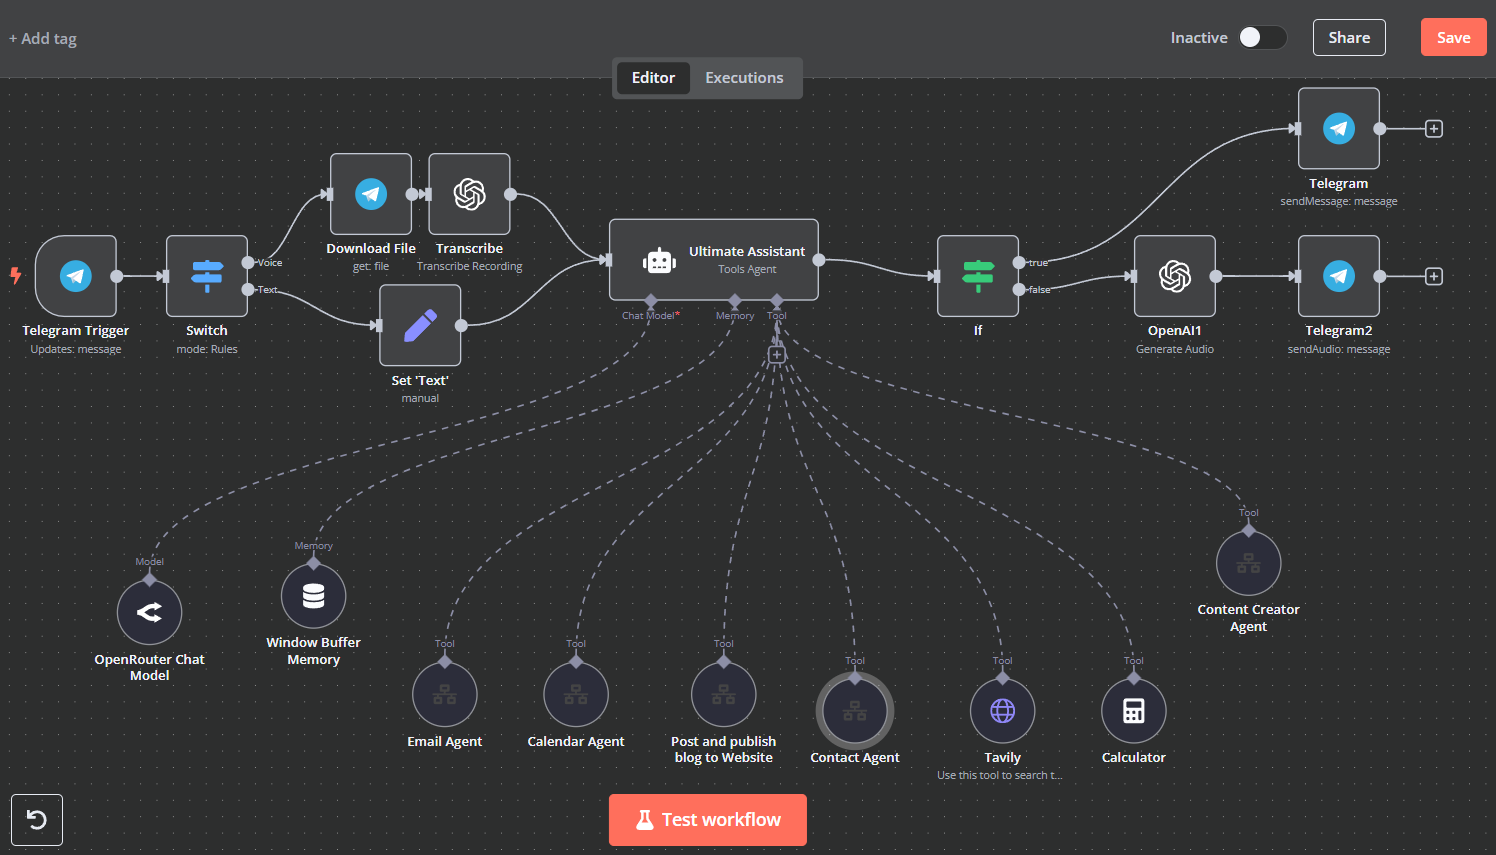
\includegraphics[width=1\textwidth]{images/4chatbot01.png}
    \caption{Workflow trợ lý ảo Telegram}
    \end{figure}


\subsection{Phân tích chi tiết công dụng và ưu điểm}

\subsubsection{Công dụng chính}
\begin{enumerate}
    \item \textbf{Trợ lý đa chức năng tự động}: Hệ thống hoạt động như một trợ lý cá nhân/văn phòng tự động xử lý nhiều loại tác vụ khác nhau.
    
    \item \textbf{Tích hợp đa nền tảng}: Kết nối Telegram làm giao diện người dùng với các dịch vụ Gmail, Google Calendar, Airtable và công cụ tìm kiếm.
    
    \item \textbf{Xử lý ngôn ngữ tự nhiên}: Người dùng có thể giao tiếp bằng văn bản hoặc giọng nói tự nhiên, không cần câu lệnh cụ thể.
    
    \item \textbf{Tự động hóa công việc hàng ngày}:
    \begin{itemize}
        \item Quản lý email: gửi, lấy, dán nhãn, tạo bản nháp
        \item Quản lý lịch: tạo, xóa, cập nhật sự kiện và cuộc họp
        \item Quản lý danh bạ: lưu trữ và truy xuất thông tin liên hệ
        \item Tạo nội dung: viết và xuất bản bài blog dựa trên nghiên cứu
    \end{itemize}
\end{enumerate}

\subsubsection{Ưu điểm nổi bật}
\begin{enumerate}
    \item \textbf{Kiến trúc module hóa}: Mỗi chức năng được phân tách thành agent riêng biệt, dễ bảo trì và mở rộng.
    
    \item \textbf{Tự động định tuyến tác vụ}: Hệ thống tự nhận diện yêu cầu và chuyển đến agent phù hợp.
    
    \item \textbf{Sử dụng LLM tiên tiến}: OpenRouter và OpenAI đảm bảo khả năng hiểu và xử lý ngôn ngữ tự nhiên chất lượng cao.
    
    \item \textbf{Xử lý lỗi thông minh}: Các agent đều có xử lý lỗi (error handling) để đảm bảo trải nghiệm người dùng mượt mà.
    
    \item \textbf{Cá nhân hóa cao}: Kết nối với tài khoản cá nhân của người dùng (email, lịch, danh bạ).
    
    \item \textbf{Đa dạng đầu vào}: Xử lý cả tin nhắn văn bản và ghi âm, tăng tính linh hoạt.
    
    \item \textbf{Tương tác hai chiều}: Cung cấp phản hồi kịp thời qua tin nhắn hoặc file âm thanh.
\end{enumerate}

\subsection{Hướng dẫn thiết lập credentials}

\subsubsection{Tổng quan về credentials cần thiết}
Để thiết lập toàn bộ hệ thống chatbot Ultimate Assistant, bạn cần cấu hình các xác thực (credentials) cho các dịch vụ sau:

\begin{itemize}
    \item Telegram Bot API
    \item OpenAI/OpenRouter API
    \item Google (Gmail và Calendar)
    \item Airtable
    \item Tavily Search API
\end{itemize}

Dưới đây là hướng dẫn chi tiết cách thiết lập từng loại credential:

\subsubsection{\underline{Telegram Bot API}}
\textbf{Mục đích}: Cho phép chatbot tương tác với người dùng qua Telegram.

\textbf{Cách thiết lập}:
\begin{enumerate}
    \item Mở Telegram và tìm kiếm \texttt{\href{https://telegram.me/BotFather}{@BotFather}}
    \item Gửi lệnh \texttt{/newbot} và làm theo hướng dẫn để tạo bot mới
    \item Đặt tên cho bot và username (phải kết thúc bằng ``bot'')
    \item BotFather sẽ cung cấp token API (dạng \texttt{123456789:ABCdefGhIJKlmNoPQRsTUVwxyZ})
    \item Trong n8n:
    \begin{itemize}
        \item Vào ``Credentials'' > ``New'' > ``Telegram API''
        \item Nhập Bot Token API đã nhận được
        \item Lưu credential với tên (ví dụ: ``Telegram account Hai'')
    \end{itemize}
\end{enumerate}

\subsubsection{\underline{OpenAI/OpenRouter API}}
\textbf{Mục đích}: Cung cấp mô hình ngôn ngữ (LLM) để chatbot hiểu và tạo phản hồi.

\paragraph{OpenAI API:}
\begin{enumerate}
    \item Đăng ký tài khoản tại \href{https://platform.openai.com/}{OpenAI}
    \item Truy cập ``API Keys'' và tạo key mới
    \item Trong n8n:
    \begin{itemize}
        \item Vào ``Credentials'' > ``New'' > ``OpenAI API''
        \item Nhập API Key
        \item Lưu credential với tên (ví dụ: ``OpenAi account'')
    \end{itemize}
\end{enumerate}

\paragraph{OpenRouter API} (thay thế cho OpenAI): thay đổi nhiều model LLM 
\begin{enumerate}
    \item Đăng ký tại \href{https://openrouter.ai/}{OpenRouter}
    \item Tạo API key mới
    \item Trong n8n:
    \begin{itemize}
        \item Vào ``Credentials'' > ``New'' > ``OpenRouter API''
        \item Nhập API Key
        \item Lưu credential với tên (ví dụ: ``OpenRouter account'')
    \end{itemize}
\end{enumerate}

\subsubsection{\underline{Google (Gmail và Calendar)}}
\textbf{Mục đích}: Cho phép chatbot truy cập và quản lý email và lịch.

\textbf{Thiết lập Google OAuth2}:
\begin{enumerate}
    \item Truy cập \href{https://console.cloud.google.com/}{Google Cloud Console}
    \item Tạo project mới hoặc chọn project sẵn có
    \item Đi tới ``APIs \& Services'' > ``Library''
    \item Kích hoạt các API: Gmail API và Google Calendar API
    \item Đi tới ``OAuth consent screen'':
    \begin{itemize}
        \item Chọn loại người dùng (External/Internal)
        \item Nhập thông tin ứng dụng (tên, email liên hệ)
        \item Thêm scopes cần thiết: Gmail (send, read, modify) và Calendar (read, write)
    \end{itemize}
    \item Tạo OAuth2 credentials:
    \begin{itemize}
        \item Đi tới ``Credentials'' > ``Create Credentials'' > ``OAuth client ID''
        \item Chọn Application Type: ``Web application''
        \item Thêm Redirect URI: URL từ n8n (thường có dạng \url{https://your-n8n-instance.com/rest/oauth2-credential/callback})
    \end{itemize}
    \item Trong n8n:
    \begin{itemize}
        \item Vào ``Credentials'' > ``New'' > ``OAuth2 API'' (cho Gmail hoặc Google Calendar)
        \item Nhập Client ID và Client Secret từ Google Cloud
        \item Nhập các scopes cần thiết
        \item Nhấn ``Connect'' và xác thực với tài khoản Google của bạn
        \item Lưu credentials với tên phù hợp (ví dụ: ``Gmail account'', ``Google Calendar account'')
    \end{itemize}
\end{enumerate}

\subsubsection{\underline{Airtable}}
\textbf{Mục đích}: Lưu trữ và quản lý thông tin liên hệ.

\textbf{Thiết lập Airtable API}:
\begin{enumerate}
    \item Đăng nhập vào \href{https://airtable.com/}{Airtable}
    \item Tạo một base mới với bảng ``Contacts'' chứa các trường: name, email, phoneNumber
    \item Truy cập ``Account'' > ``Developer Hub'' > ``Personal Access Tokens''
    \item Tạo token mới với quyền truy cập phù hợp
    \item Trong n8n:
    \begin{itemize}
        \item Vào ``Credentials'' > ``New'' > ``Airtable API''
        \item Nhập API Key
        \item Lưu credential với tên phù hợp
    \end{itemize}
    \item Lấy Base ID:
    \begin{itemize}
        \item Mở Airtable base của bạn
        \item Xem URL: \texttt{https://airtable.com/[BASE\_ID]/[TABLE\_ID]/[VIEW\_ID]}
        \item Lưu lại BASE\_ID để sử dụng trong workflow
    \end{itemize}
\end{enumerate}

\subsubsection{\underline{Tavily Search API}}
\textbf{Mục đích}: Cho phép chatbot tìm kiếm thông tin trên web.

\textbf{Thiết lập Tavily API}:
\begin{enumerate}
    \item Đăng ký tài khoản tại \href{https://tavily.com/}{Tavily}
    \item Nhận API key từ dashboard
    \item Trong workflow n8n:
    \begin{itemize}
        \item Tại nút HTTP Request Tool, nhập trực tiếp API key vào JSON body:
    \end{itemize}
\end{enumerate}

\begin{lstlisting}[language=json, basicstyle=\small\ttfamily]
{
  "api_key": "tvly-YOUR_API_KEY",
  "query": "{searchTerm}",
  "search_depth": "basic",
  "include_answer": true,
  "topic": "news",
  "include_raw_content": true,
  "max_results": 3
}
\end{lstlisting}

\subsubsection{\underline{Kiểm tra và xác minh credentials}}
Sau khi cài đặt tất cả credentials:
\begin{itemize}
    \item Kiểm tra từng workflow để đảm bảo nó được liên kết với credential đúng
    \item Thực hiện kiểm tra kết nối cho mỗi credential trong n8n
    \item Chạy thử từng workflow thành phần trước khi tích hợp vào hệ thống chính
\end{itemize}

\subsubsection{\underline{Lưu ý bảo mật}}
\begin{itemize}
    \item \textbf{Không chia sẻ API keys}: Bảo vệ tất cả credentials và không chia sẻ trong code công khai
    \item \textbf{Giới hạn quyền truy cập}: Chỉ cấp quyền cần thiết cho mỗi API
    \item \textbf{Theo dõi sử dụng}: Giám sát việc sử dụng API để tránh vượt quá giới hạn
    \item \textbf{Luân chuyển keys}: Cập nhật keys định kỳ theo các thực hành bảo mật tốt nhất
    \item \textbf{Mã hóa credentials}: n8n mã hóa credentials, nhưng hãy đảm bảo máy chủ n8n được bảo mật
\end{itemize}

Với tất cả các credentials được thiết lập đúng cách, Ultimate Assistant Chatbot của bạn sẽ có thể tương tác với Telegram và điều phối tất cả các dịch vụ bên ngoài một cách liền mạch.